\documentclass[12pt,a4paper,twoside]{report}
\usepackage[utf8]{inputenc}
\usepackage[T1]{fontenc}
\usepackage[swedish,english]{babel}
\usepackage{amsmath}
\usepackage{ae}
\usepackage{units}
\usepackage{icomma}
\usepackage{color}
\usepackage{graphicx}
\usepackage{bbm}
\usepackage{textcomp}
\usepackage{url}
\usepackage{verbatim}
\usepackage[font=footnotesize,margin=1cm,labelfont=bf,format=hang]{caption}
\usepackage{subfig}
\usepackage{marvosym}
\usepackage{eso-pic}
\usepackage{fancyhdr}
\usepackage{amssymb}
\usepackage{geometry}
\usepackage{titlesec}
\usepackage{boxedminipage}
\usepackage{parskip}
\usepackage{cite}
\usepackage[table]{xcolor} % Färg i tabeller, använd exv \cellcolor{red}
\usepackage{xcolor}
\usepackage{listings}
\usepackage{mcode} % För m-filer, använd exv \lstinputlisting[firstline=5, lastline=15]{../code/FILENAME.m}

% åäö till comments i m-filer
\lstset{
  literate={ö}{{\"o}}1
           {ä}{{\"a}}1
           {å}{{\r{a}}}1
}

% Definiera bindestreck för math mode \mhyphen
\mathchardef\mhyphen="2D

% Omdefiniera paragraph kommandot med titlesec-paketet
\titleformat{\paragraph}[hang]{\normalfont\normalsize\bfseries}{\theparagraph}{1em}{}
\titlespacing*{\paragraph}{0pt}{2mm plus 1mm minus .2mm}{-1mm}

% -- Omdefiniera hur latex hanterar floats (figurer)
\renewcommand{\topfraction}{0.9}	
    \renewcommand{\bottomfraction}{0.8}	
    \setcounter{topnumber}{2}
    \setcounter{bottomnumber}{2}
    \setcounter{totalnumber}{4} 
    \setcounter{dbltopnumber}{2} 
    \renewcommand{\dbltopfraction}{0.9}	
    \renewcommand{\textfraction}{0.07}	
    \renewcommand{\floatpagefraction}{0.7}	
	% floatpagefraction MUST be less than topfraction !!
    \renewcommand{\dblfloatpagefraction}{0.7}
% --

%\linespread{1.3}
%\setcounter{secnumdepth}{-1}

\setlength{\headheight}{15pt}


\newcommand\BackgroundPic{
\numberwithin{equation}{section}
\put(-4,0){
\parbox[b][\paperheight]{\paperwidth}{
\includegraphics[width=\paperwidth,
keepaspectratio]{images/logo.eps}
\vfill
}}}

%\setlength{\parindent}{0mm}
% Geometri på titelsida
\newgeometry{margin=0.5in}

\begin{document}
% Skapa "vattenmärke"
\AddToShipoutPicture*{\BackgroundPic}
\begin{titlepage}

\mbox{}
\vfill

% Bild på titelsidan?

\Huge
\textbf{Väderparametrars inverkan på \\energiförluster i en fastighet - \\en studie av värmeflöden}

\normalsize
% Teknisk Fysik?
\textit{Kandidatarbete inom civilingenjörsprogrammen Teknisk Fysik och Elektroteknik}

\vspace{1.5cm}

\large
Erik Ahlqvist\\
Ylva Dahl\\
Mats Lindström\\
Dan Ståby\\

\vspace{1cm}

\normalsize
Institutionen för Teknisk Fysik\\
CHALMERS TEKNISKA HÖGSKOLA\\
Göteborg, Sverige, 2012\\
% Vilket nummer har arbetet?
Kandidatarbete TIFX-02-12-19

\end{titlepage}

%\setlength{\parindent}{0pt}
%\setlength{\parskip}{10pt}

\newpage
% Vilken geometri?
\newgeometry{margin=3cm, headheight=15pt}

%--- Sidhuvud & sidfot
	\pagestyle{fancy}
	\chead[\footnotesize Väderparametrars inverkan på energiförluster i en fastighet -- en studie av värmeflöden]{\nouppercase{\footnotesize \leftmark}}
        \lhead[]{}
        \rhead[]{}
%---
	
\newpage
\thispagestyle{empty}
\mbox{}
\vspace{6cm}

\begin{center}
\large
KANDIDATARBETE TIFX-02-12-19\\
\vspace{1cm}
\Huge
Väderparametrars inverkan på \\energiförluster i en fastighet -- \\en studie av värmeflöden\\
\vspace{1cm}
\normalsize
Kandidatarbete vid Teknisk Fysik\\
\vspace{1cm}
Erik Ahlqvist, Ylva Dahl, Mats Lindström, Dan Ståby\\
\vfill
Institutionen för Teknisk Fysik
\end{center}

\newpage
\pagenumbering{gobble}

\chapter*{Förord}

% Förord här

Vi vill rikta ett varmt tack till alla som har hjälp oss att möjliggöra detta projekt. 

Vi vill speciellt tacka Angela Sasic, lektor på Institutionen för Byggnadsteknologi på Chalmers, för att ha bistått oss med litteratur så väl som modeller, NN och NN, NÅGOT på SMHI för information om prognosstyrning av inomhusklimatet och sitt resonemang kring sådana modeller, NN, som generöst har delat sin datormodell med världen och tillåtit oss att NÅGOT.

Vidare vill vi tacka Peter Särneö, teknisk chef för fastigheten på Walleriusgatan, som ställt upp på möten och besvarat våra frågor, Peter Apell för korrekturläsning och många användbara kommentarer på små och stora texter, handledarna på Fackspråk som genom sin kunskap väglett och utbildat oss i processen kring att skriva en större rapport,

Vi vill även tacka Brett W. Bader och Tamara G. Kolda vid Sandia National Laboratories för deras
matlabkod ``Tensor Toolbox'' som har används vid lösning av finita element av Navier-Stokes ekvationer.

Avslutningsvis vill vi rikta ett stort tack till vår handledare Magnus Karlsteen som NÅGOT.

%\newpage


\selectlanguage{swedish}
\begin{abstract}
% På svenska här

% Avsikten med arbetet
Avsikten är att undersöka hur energi flödar genom en fastighet beroende på vilket väder det är. Detta syftar i sin tur till att kunna minska fastighetens löpande energikostnader samt att få ett jämnare inomhusklimat. Därför presenteras även några olika metoder samt kostnadsförslag till dessa för hur energiflödena kan minskas. De åtgärder som behandlas är isolering av de ännu oisolerade väggarna, SMHI:s prognosstyrningstjänst samt termostater inne i lägenheterna.

% metoden som användes
Fastigheten har delats upp i byggnadsskalet med väggar, tak, fönster och grund där energiflödet undersökts genom var och en av delarna för sig. Solinstrålning genom fönstren och ofrivillig ventilation, alltså drag på grund av vind, behandlas också separat.

Termisk energi överförs genom strålning, konvektion och ledning och i varje beräkning av fastighetens energiflöde är det viktigt att undersöka alla sådana flöden. För detta har vi använt både analytiska beräkningsmetoder och simuleringar i Matlab och Comsol Multiphysics. En återkommande beräkningsmetod är finita elementmetoden och givetvis är även värmeledningsekvationen en central del.

% vilka resultat som erhölls samt 
Det visade sig att de främsta källorna till energiförluster är fönstren och ofrivillig ventialtion. Att ta hänsyn till solinstrålning ger en besparing på över 17 \% av energin en solig dag vilket motsvarar 4 \% av energin för alla dagar. Vinden sänker temperaturen och att ta hänsyn till den kan ge en jämnare inomhustemperatur men inte nödvändigtvis en minskning i energiåtgång. För att avgöra exakt hur mycket energi som försvinner vid vind behöver ett trycktest göras.

Det kom också fram att de olika väggarnas reaktionstid vid ett väderomslag varierade kraftigt – från under 4 timmar till över 100 och det behöver man ta hänsyn till i injusteringen av sitt reglersystem. 

% vilka slutsatser som dragits

% INTE DISKUSSION! 

%\newpage

\end{abstract}

\selectlanguage{english}
\begin{abstract}

The purpose of this project was to investigate the flow of energy through a building due to the effect of the weather. Another objective with this investigation is, if possible, to reduce the heating costs of the building and to get a more stable indoor climate. Hence, there is also an included comparison of some other energy saving methods. Weather-forecast-based control of the heating system is a commercial product supplied by e.g. SMHI. Other considerations investigated for reducing heating costs are insulations the walls, or to mount electrical thermostat devices on the radiators in the building.

The different parts of the building have been separated to wall, windows, roof and foundation. This made the quantification of energies easier to compute. Solar irradiation through windows and infiltration losses due to involuntary ventilation are discussed. 

Thermal energy is transmitted through radiation, convection and heat conduction. These three fundamental physical processes have been used in the investigation of every subflow. To evaluate the differential equations and physical properties, both analytical and numerical methods were used. These include the finite element method which were implemented \emph{ad hoc} in \emph{Matlab}. The softwares \emph{Comsol Multiphysics} have also been used to evaluate differential equations with the finite element method. 

The models in this Bachelor’s thesis showed that the primary sources of
energy expense is radiation through windows and infiltration losses. It
is also possible to reduce the energy consumption by at least $\unit[17]{\%}$ by adjusting
the heating system of the building to account for solar irradiation a sunny day. This means
that it is possible to save over $\unit[4]{\%}$ of the energy expense through a whole year.
The wind lowers the temperature inside. This means that it is probaly not possible to save energy
by taking consideration of wind's effect.
To completely understand how much energy is lost due to infiltration a
blow door test needs to be performed.


Another main conclusion of this project was that the different walls had very different reaction times when the weather changed rapidly. It varied from below 4 hours up to above 100 hours, and it is important to have this in mind when adjusting the heating system of the building.

\end{abstract}

\selectlanguage{swedish}

\newpage


\pagenumbering{roman}
\setcounter{tocdepth}{3} % Så att subsubsection syns i toc
\setcounter{secnumdepth}{3} % Numrerade subsubsections
\tableofcontents
\newpage

\pagenumbering{arabic}
\setcounter{page}{1}


%--- input går här:

% Inledning
\section{Inledning}



%Teori
\section{Teori}

För att beskriva fysikaliska fenomen används olika matematiska modeller. I våra simuleringar av vädrets inverkan på fastighetens energiflöden använder vi flera olika beräkningsmetoder. I det här avsnittet presenterar vi härledningar av de fysikaliska fenomen och beräkningsmetoder projektet använder sig av. Vi går också igenom definitioner av, för projektet, centrala begrepp.


\subsection{Värmeledning}
Konduktion. Det pågår ständigt värmetransport från kalla till varma sidor. Värmetransporten är proportionell mot temperaturskillnaden över konstruktionen. Konduktion, eller ledning genom ett material, här värmeledning innebär att värme flyttar sig inom ett material, utan att materialet i sig rör sig eller flyttar sig. Konduktiviteten, eller värmeledningsförmågan, betecknad kappa inom fysiken eller lambda inom byggsektorn är en materialegenskap. Eftersom överföring av värme i form av ledning är den enklaste överföringen är det den som lambda värdet bygger på. För att bestämma lambdavärdet för ett material utsätter man det för en temperaturskillnad och mäter den värmemängd som passerar genom materialet per tidsenhet. Då värmeöverföring via konvektion samt strålning är så pass svår att behandla matematiskt så ingår dessa i lambdavärdet som är väldigt enkelt att jobba med matematiskt. $q=k \nabla \cdot T$ vilket ger oss $Q=U \delta \cdot T$ och därifrån kan vi lösa ut U-värdet som $U = frac{Q}{\delta\ cdot T}$. Värmeledningsförmågan påverkas av materialets densitet, porositet, temperatur samt fuktighet. Fuktkorrigering görs, enligt vissa framställda värden. Värmemotstånd, R beräknas utifrån lambdavärdet.

\begin{equation}
Ri=\frac{d}{lambda}
\end{equation}

Överföringsmotstånd. Man påför sedan Rsi samt Rse, utsida samt insida. Beror på både strålnings samt konvektion. U-värdet beräknas som inversen av R-värdet. Har man olika material handlar det om att summera ihop 1/r.

\section{Svartkroppsstrålning}
\label{sec:blackbody}



Alla objekt reflekterar, absorberar och transmitterar ljus. De kroppar som varken reflekterar eller transmitterar något ljus utan absorberar 100\% kallas konventionellt för svartkroppar. Detta är en teorektisk konstruktion då perfekta svartkroppar inte existerar men trots detta kan en sådan användas som en god modell i flera fysikaliska tillämpningar. Den energi som absorberats strålas ut i form av svartkroppsstråling vars frekvensspektum bestäms av kroppens temperatur när kroppen är i termisk jämvikt med sin omgivning. Den totala utstrålade energin per tidsenhet fås ur Stefan-Boltzmanns lag


\begin{equation}\boxed{ \; \; \;
j^{\star} = \sigma T^{4}
\; \; \; }
\end{equation}

\noindent
där $\sigma$ är Stefan-Boltzmanns konstant som mäts i $\unit{s^{-1}m^{-2}K^{-4}}$ och $T$ är kroppens temperatur vid termisk jämvikt.

\subsection{Härledning}
% av stefan-boltzmanns lag
% med hål i en låda
% kolla i termoboken
I en låda med fotoner kan den totala energin inne i lådan beskrivas som 
\begin{equation}
\frac{U}{V}=\frac{8\pi^5}{15}\frac{(kT)^4}{(hc)^3}
\end{equation}

vilket fås ur Plancks spektrum.\cite{schroeder00}

Sedan görs ett litet hål i lådan, så att några av fotonerna kan slippa ut. Sannolikhet att fotoner med kort respektive lång våglängd ska slippa ut är samma som fördelningen mellan dem inne i lådan, eftersom de har samma hastighet.

\begin{figure}[hpbt]
\centering
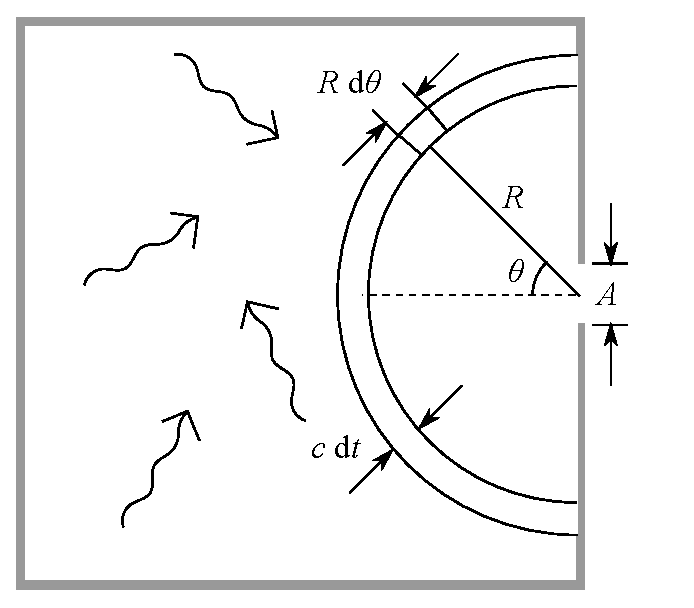
\includegraphics[height=0.3\textheight]{images/blackbody_box.eps}
\caption{\label{fig:box}{Fotonerna som lämnar lådan har en liten stund tidigare befunnit sig i samma hemisfär inne i lådan.}}
\end{figure}

Den totala mängden strålning som kommer ut kan då beräknas genom att tänka sig att de fotoner som når fram till hålet under en kort tidsperiod, $\mathrm{d}t$, alla befann sig i samma hemisfär inne i lådan för en liten stund sedan, se figur \ref{fig:box}. Tjockleken på den tänkta hemisfären är $c\mathrm{d}t$. Hemisfärens radie, $R$, beror givetvis på hur långt bak i tiden vi tittar.

Ett volymelement av hemsfären ges av
\begin{equation}
V=(R\mathrm{d}\theta) \times (R\sin\theta\mathrm{d}\phi) \times (c \mathrm{d}t).
\end{equation}

Energitäthetenför fotonerna i volymelementet är således
\begin{equation}
E_\text{v.e.}=\frac{U}{V} c \mathrm{d}t R^2 \sin\theta \mathrm{d}\theta \mathrm{d}\phi.
\end{equation}

Men endast den andel av fotonerna som har rätt riktning kommer ut genom lådans öppning. Sannoliketen för att en foton har rätt riktning är
\begin{equation}
P(\text{rätt riktning})=\frac{A\cos\theta}{4\pi R^2}
\end{equation}

där A är hålets area. Den totala energin som strålar ut ur hålet från det lilla volymselementet är alltså 
\begin{equation}
\frac{A\cos\theta}{4\pi}\frac{U}{V} c\mathrm{d}t \sin\theta\mathrm{d}\theta \mathrm{d}\phi
\end{equation}

vilket ger en total energiutstrålning på
\begin{equation}
\frac{A}{4}\frac{U}{V}c \mathrm{d}t
\end{equation}


\subsection{Konvektion}
\label{section:convection}
I fasta ämnen går det utmärkt att approximera värmeflöde enbart med hjälp
av värmeledningsekvationen. Detta håller dock ej lika bra för fluider, det vill säga
material som deformeras då de utsätts för tryck.
Under dessa förhållanden
måste det tas hänsyn till konservation av massa, energi samt rörelsemoment.
För att härleda giltiga differentialekvationer som beskriver en fluids rörelse används ofta sambandet

\begin{equation}
\label{eq:convection:reynolds}
\frac{dB}{dt} = \frac{d}{dt}\left( \int_{V} \frac{dB}{dm} \rho dV \right) + \int_{\partial V} \frac{dB}{dm} \rho \left( \mathbf{v} \cdot \mathbf{n} \right)dA,
\end{equation}

där $B$ är en godtycklig egenskap av fluiden, exempelvis dess rörelsemängd, V är den så kallade kontrollvolymen (omfattande ett godtyckligt valt område), $\partial V$ är denna kontrollvolyms rand, $\rho$ är fluidens densitet, $\mathbf{v}$ är fluidens hastighetsvektor och $\mathbf{n}$ är normalvektorn till randen. Detta samband benämns vanligen Reynolds transportteorem\footnote{För närmare beskrivning och härledning, se White, 2011 \cite{white11}}.

Sätt $B = m$ där $m$ är fluidens massa (oberoende av tiden) och låt $V$ vara en tidsoberoende volym. Ett uttryck för masskonservering erhålls:

\begin{equation}
\label{eq:convection:masscon}
\int_V \frac{\partial \rho}{\partial t} dV + \int_{\partial V} \rho \left( \mathbf{v} \cdot \mathbf{n} \right) dA = 0
\end{equation}

Första termen i detta uttryck beskriver förändringar i densiteten inom kontrollvolymen medan andra termen omfattar alla flöden in och ut genom kontrollvolymens rand. För masskonservering krävs alltså att summan av dessa termer ska vara noll. Den andra termen kan, vid diskreta flödesmängder, även skrivas som

\begin{equation}
\label{eq:convection:discrete}
\int_{\partial V} \rho \left( \mathbf{v} \cdot \mathbf{n} \right) dA = \sum_i \left( \rho \mathbf{v}_i\cdot \mathbf{A}_i \right)_{ut} - \sum_i \left( \rho \mathbf{v}_i\cdot \mathbf{A}_i \right)_{in}
\end{equation}

\begin{figure}[hpbt]
\centering
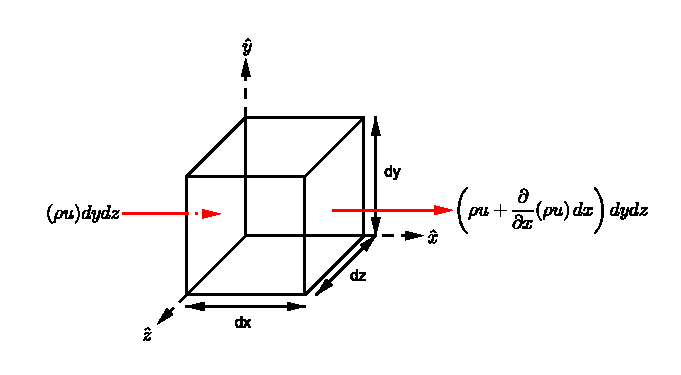
\includegraphics[scale=1]{images/massflowcube.eps}
\caption{\label{fig:massflowcube} Infinitesimal kontrollvolym för derivering av bevaranderelationer, här med massflödet exemplifierat}
\end{figure}

Betrakta nu en infinitesimal kontrollvolym som den i figur \ref{fig:massflowcube}. In- och utflödena kan här approximeras till endimensionella flöden och \eqref{eq:convection:masscon} reduceras till

\begin{equation}
\label{eq:convection:massconinf}
\int_V \frac{\partial \rho}{\partial t} dxdydz + \frac{\partial}{\partial x}\left( \rho u \right)dxdydz + \frac{\partial}{\partial y}\left( \rho v \right)dxdydz + \frac{\partial}{\partial z}\left( \rho w \right)dxdydz = 0
\end{equation}

vilket, om dxdydz tas bort, kan förenklas som

\begin{equation}
\label{eq:convection:continuity}
\frac{\partial \rho}{\partial t} + \nabla \cdot \left( \rho \mathbf{v} \right) = 0
\end{equation}

Om inkompressibilitet antas ($\rho$ = konstant) reduceras denna ekvation ytterligare till

\begin{equation}
\label{eq:convection:continuityinc}
\nabla \cdot \mathbf{v} = 0
\end{equation}

Detta är kontinuitetsekvationen för inkompressibla fluider.

Betrakta åter \eqref{eq:convection:reynolds} och sätt nu $B = m\mathbf{v}$. På samma vis som kontinuitetsekvationen \eqref{eq:convection:continuityinc} härleddes, fås för det infinitesimala volymelementet i figur sambandet

\begin{eqnarray}
\label{eq:convection:linear}
\sum \mathbf{F} & = & \frac{\partial}{\partial t} \left( \int_V \mathbf{v} \rho dV \right) + \sum_i \left( \dot{m}_i \mathbf{v}_i \right)_{ut} - \sum_i \left( \dot{m}_i \mathbf{v}_i \right)_{in}\nonumber\\
& = &\left(\frac{\partial}{\partial t} \left( \rho\mathbf{v} \right) + \frac{\partial}{\partial x}\left( \rho u \mathbf{v}\right) + \frac{\partial}{\partial y}\left( \rho v \mathbf{v}\right) + \frac{\partial}{\partial z}\left( \rho w \mathbf{v}\right)\right)dxdydz
\end{eqnarray}

ty enligt Newtons andra lag är tidsderivatan av rörelsemängden $m\mathbf{v}$ lika med summan av alla krafter som verkar på kroppen. $\dot{m}_i$ betecknar här massflödet $\rho\mathbf{v}_i\cdot\mathbf{A}_i$.

Det sista högerledet kan skrivas om som

\begin{equation}
\left( \mathbf{v}\left[ \frac{\partial \rho}{\partial t} + \nabla\cdot \rho \mathbf{v}\right] + \rho\left[ \frac{\partial \mathbf{v}}{\partial t} + u\frac{\partial\mathbf{v}}{\partial x} + v\frac{\partial\mathbf{v}}{\partial y} + w\frac{\partial\mathbf{v}}{\partial z} \right]\right)dxdydz.
\end{equation}

Första termen inom hakparentes är kontinuitetsekvationen \eqref{eq:convection:continuity} och går alltså bort. Den andra hakparentesen motsvarar något som kallas materiederivata. Man kan visa att 

% OBS, blandat tensorer och vektorer!
\begin{equation}
\label{eq:convection:material}
\frac{d\mathbf{v}}{dt} = \frac{\partial \mathbf{v}}{\partial t} + \mathbf{v}_i\frac{\partial \mathbf{v}}{\partial x_i}
\end{equation}

och därmed reduceras \eqref{eq:convection:linear} till

\begin{equation}
\label{eq:convection:linearfinal}
\sum \mathbf{F} = \rho \frac{d\mathbf{v}}{dt}dxdydz.
\end{equation}

Summan av de på volymen verkande krafterna måste nu utvecklas. Dessa krafter uppstår på grund av gravitation, tryck och viskositet. Andra krafter, såsom från elektromagnetiska fält, kan i sammanhanget anses vara försumbara. Gravitationskraften $\mathbf{F}_g$ beskrivs för den infinitesimala volymen med $\rho \mathbf{g} dxdydz = \rho g dxdydz \hat{z}$. Tryckkraften $\mathbf{F}_p$, i sin tur, ges av $-\nabla p dxdydz$. Viskositetskraften $\mathbf{F}_{visc}$ är lite besvärligare att sammanställa. Anta att volymen är en Newtonsk fluid, det vill säga stresstensorn $\tau$ är linjärt proportionell mot hastighetsgradienten $\nabla\mathbf{v}$ med proportionaltitetskonstanten $\mu$, $\tau = \mu \nabla \mathbf{v}$. 

% Hur härleda viskositetsbidraget

Vi har alltså ekvationssystemet

\begin{eqnarray}
\frac{du}{dt} & = & -\frac{\partial p}{\partial z} \nonumber\\
\frac{dv}{dt} & = & -\frac{\partial p}{\partial z}\\
\frac{dw}{dt} & = & \rho g -\frac{\partial p}{\partial z} \nonumber
\end{eqnarray}


För homogena inkompressibla fluider i två dimensioner gäller då ekvationerna
\eqref{eq:convection:continuity}, \eqref{eq:convection:momentumx},
\eqref{eq:convection:momentumz} samt \eqref{eq:convection:energy}. Här
är $\mathbf{v} = (u,w)$ hastighetsvektorn, $\alpha$ är den termiska
diffusiviteten, $\nu$ är den kinematiska viskositeten, $p$ är trycket,
$\rho$ är densiteten, $g$ är den lokala tyngdaccelerationen
och slutligen är $\rho_0$ referensdensiteten.

\begin{equation}
\label{eq:convection:momentumx}
\frac{\partial u}{\partial t} + \mathbf{v}\cdot\nabla u = 
-\frac{1}{\rho_0}\frac{\partial p}{\partial x} + 
\nu\Delta u
\end{equation}

\begin{equation}
\label{eq:convection:momentumz}
\frac{\partial w}{\partial t} + \mathbf{v}\cdot\nabla w = 
-\frac{1}{\rho_0}\frac{\partial p}{\partial z} + \nu\Delta w - \frac{\rho}{\rho_0}g
\end{equation}

\begin{equation}
\label{eq:convection:energy}
\frac{\partial T}{\partial t} + \mathbf{v}\cdot\nabla T = \alpha\Delta T
\end{equation}

\subsubsection{Boussinesq approximation}

För flytkraftsdrivet flöde kan det vara lämpligt att använda sig av
Boussinesq approximation. Denna säger att det enda som påverkar trycket är
tyngdaccelerationen. Genom detta är det möjligt att sätta upp uttryck för densiteten
och tryckderivatorna enligt ekvationerna \eqref{eq:convection:density}
och \eqref{eq:convection:pressurez}. Här är
$\beta$ den volymetriska expansionskonstanten och
$T_0$ temperaturen som råder vid referensdensiteten $\rho_0$.

\begin{equation}
\label{eq:convection:density}
\rho = \rho_0[1-\beta(T-T_0)]
\end{equation}

\begin{equation}
\label{eq:convection:pressurez}
\frac{\partial p}{\partial z} = -\rho_0g
\end{equation}



\subsection{Finita element av inkompressibel fluid}

För att lösa Navier-Stokes ekvationer kan lämpligen en datormodell användas.
Här består denna modell av ett system uppsatt med Galerkins metod.
I denna lösning så begränsar vi dock oss till att enbart behandla statiska flöden
vilket genomförs genom att sätta alla tidsderivator till noll.

För att hantera trycket i \eqref{eq:convection:continuity}-\eqref{eq:convection:energy} används den tidigare nämnda Boussinesq approximation
samt penalty metoden för att göra hastighetsvektorn källfri och uppfylla
kontinuitetsekvationen. Det finns således inget direkt behov av att räkna ut trycket.
Vid användning av många sorters elementtyper som inte uppfyller Babuska-Brezzikriteriet
är detta dessutom nödvändigt då det annars kan bildas oönskade trycknoder. 
En annan möjlighet är att välja divergensfria element. \cite{babuska1973}\cite{segal2011}

Genom penaltymetoden beskrives här trycket som $p$ enligt ekvation
\eqref{eq:femconvection:penalty}. Här är $p_s$ någon form av idealt statiskt
tryck som är önskat. Detta tryck följer Boussinesq approximation. Med dessa
idealiseringar kan differentialekvationerna sättas upp igen. \cite{heinrich88}\cite{taylor79}
Som kan ses så leder den godtyckliga penaltyparametern $\lambda$ till att justera trycket
om hastighetsfältets divergens ej är identiskt noll. I viss litteratur anges 
det att penaltyparametern skall vara i storleksordningen $10^7$ men att den
är väldigt applikationsberoende. En för liten vald penaltyparameter leder till att
trycket inte elimineras. Andra problem uppstår vid en för stor parameter. Ekvationssystemet
kan bli svårlöst och få stabilitetsproblem när parametern blir
för stor i jämförelse med de andra delarna i differentialekvationen.\cite{reddy93}\cite{roy05}\cite{basak04}\cite{segal2011}

\begin{equation}
\label{eq:femconvection:penalty}
p = p_s - \lambda\nabla\cdot\mathbf{v}
\end{equation}

\noindent
Fortsatt skall trycket deriveras med avseende på de rumsliga variablerna vilket möjliggör
att eliminera trycket från differentialekvationerna. Dessa deriveringar kan ses i ekvation
\eqref{eq:femconvection:partx} samt \eqref{eq:femconvection:partz}. Notera att det statiska trycket
$p_s$ ej beror på $x$ vilket resulterar i att derivatan är noll.

\begin{equation}
\label{eq:femconvection:partx}
\frac{\partial p}{\partial x} = \frac{\partial p_s}{\partial x} -
\frac{\partial}{\partial x} \lambda\nabla\cdot\mathbf{v} = -
\frac{\partial}{\partial x} \lambda\nabla\cdot\mathbf{v}
\end{equation}

\begin{equation}
\label{eq:femconvection:partz}
\frac{\partial p}{\partial z} = \frac{\partial p_s}{\partial z} -
\frac{\partial}{\partial z} \lambda\nabla\cdot\mathbf{v} =
-g\rho_0 - \frac{\partial}{\partial z} \lambda\nabla\cdot\mathbf{v}
\end{equation}

\noindent
Detta förs in i momentekvationerna vilket ger ekvationerna \eqref{eq:femconvection:u} -
\eqref{eq:femconvection:T}. Här är det ekvationssystem som syftar att lösas.

\begin{equation}
\label{eq:femconvection:u}
\mathbf{v}\cdot\nabla u =
\frac{\lambda}{\rho_0}\nabla\cdot\mathbf{v} +
\nu\Delta u
\end{equation}

\begin{equation}
\label{eq:femconvection:w}
\mathbf{v}\cdot\nabla w =
\frac{\lambda}{\rho_0}\nabla\cdot\mathbf{v} + \nu\Delta w +g\beta(T-T_0)
\end{equation}

\begin{equation}
\label{eq:femconvection:T}
\mathbf{v}\cdot\nabla T = \alpha\Delta T
\end{equation}

\subsubsection{Svag formulering}

En finita elementlösning med Galerkins metod kräver att problemet reduceras till
ett ekvivalent variationsproblem. Här söks $T\in\Phi$, $u\in\Phi$ och
$w\in\Phi$ som uppfyller ekvation \eqref{eq:femconvection:variation}. Här
betecknar brackets skalärprodukt, $\mathbf{L}$ är differentialoperatorn
som betecknar systemet av differentialekvationer som $\mathbf{L}(T,u,w) = 0$.
$\Phi$ är rummet av alla testfunktioner $\phi$ som är kontinuerliga i
definitionsmängden $\Omega$ samt vars derivator är bitvis kontinuerliga på randen
$/Gamma$. De måste även vara $L^2$ integrabla.

\begin{equation*}
\label{eq:femconvection:variation}
\langle \mathbf{L}(T,u,w), \phi \rangle = 0\mbox{,  } \forall \phi \in \Phi
\end{equation*}


\section{Optimering med Newton-Raphsons metod}

När ett ekvationssystem är ickelinjärt kan ej exakta metoder som Gausseliminering användas
för ekvationslösning. Detta stötte vi till exempel på vid finita elementlösningen
av Navier-Stokes ekvationer i avsnitt \ref{sec:femconvection}.
I dessa fall måste approximativa optimeringsmetoder utnyttjas. En sådan
metod är Newton-Raphsons metod. Denna bygger på trunkerad Taylorutveckling 
av en funktion för att linjarisera ett ickelinjärt ekvationssystem
$\mathbf{f}(\mathbf{x}) = 0$
vilket kan ses i ekvation \eqref{eq:newtonsmethod:taylor}. Här är
$\mathbf{J}_f(\mathbf{x})$ jacobianen för $\mathbf{f}(\mathbf{x})$. 

\begin{equation}
\label{eq:newtonsmethod:taylor}
\mathbf{f}(\mathbf{x} + \Delta\mathbf{x}) \approx \mathbf{f}(\mathbf{x}) +
\mathbf{J}_f(\mathbf{x})\Delta\mathbf{x}
\end{equation}

\noindent
Principen går ut på att algoritmen upprepat gissar nya lösningar där de
nya lösningarna följer den negativa jacobianen. Till en början är en god initial gissning
$\mathbf{x}_0$ ett kriterie för att Newton-Raphson skall konvergera. Därefter så beräknas
funktionsvärdet $\mathbf{f}(\mathbf{x}_0)$ samt jacobianen $\mathbf{J}_f(\mathbf{x}_0)$.
Dessa används för att beräkna nästa gissning genom att lösa
\eqref{eq:newtonsmethod:guess} och beräkna nästa $\mathbf{x}$ med
\eqref{eq:newtonsmethod:nextx}. \cite{heath2002}

\begin{equation}
\label{eq:newtonsmethod:guess}
\mathbf{J}_f(\mathbf{x}_n)\Delta\mathbf{x}_n = -\mathbf{f}(\mathbf{x_n})
\end{equation}

\begin{equation}
\label{eq:newtonsmethod:nextx}
\mathbf{x}_{n+1} = \mathbf{x}_n + \Delta\mathbf{x}_n
\end{equation}

\noindent
Itereringen bör avbrytas då ett maxantal itereringar har uppnåtts och funktionen
ej har konvergerat alternativt när felet är tillräckligt litet. En av styrkorna 
med denna algoritm är dess kvadratiska konvergens mot enkelrötter. \cite{ympa95}
En svaghet med Newton-Raphson är att det i många fall ej är möjligt att analytiskt beräkna
jacobianen. Istället måste andra algoritmer untnyttjas som till exempel finita differensmetoden
för beräkning av jacobianen. Omvägar som denna bidrar till att lösningsprocessen blir mycket
mer omständig och processorintensiv. 

\subsection{Konvergens samt konvergenskriterier}

För att enklare förstå några problem som kan uppstå med Newton-Raphsons metod kan det vara lämpligt
att repetera beviset av dess kvadratiska konvergens. Definiera en funktion $f(x)$ enligt \eqref{eq:newtonproof}.
Antag att den roten $f(x) = 0$ existerar för $x = \alpha$.

\begin{align}
f: & \mathbb{R} \to \mathbb{R} \nonumber \\
   & x \mapsto f(x) \label{eq:newtonproof}
\end{align}

\noindent
Härnäst genomförs en taylorutveckling av funktionen $f(x)$ i ekvation \eqref{eq:newtonprooftaylor}.
Den kvadratiska termen är här Lagranges restterm med parametern $\xi_n \in [\alpha, x_n]$.

\begin{equation}
\label{eq:newtonprooftaylor}
f(\alpha) = f(x_n) + f^\prime(x_n)(x_n-\alpha) + \frac{f^{\prime\prime}(\xi_n)}{2}(x_n-\alpha)^2
\end{equation}

\noindent
Nu kan förstaderivatan av $f(x_n)$ divideras över samt $f(\alpha)$ är känt att vara noll.
Efter detta identifieras $f(x_n)/f^\prime(x_n) = x_n-x_{n+1}$ och ersätts. Slutligen så ses
det i ekvation \eqref{eq:newtonqed} att $x_{n+1}-\alpha \propto (x_{n}-\alpha)^2$.

\begin{equation}
0 = \frac{f(x_n)}{f^\prime(x_n)} + \alpha - x_n + \frac{f^{\prime\prime}(\xi_n)}{2f^\prime(x_n)}(x_n-\alpha)^2
\Rightarrow
\end{equation}

\begin{equation}
\label{eq:newtonqed}
x_{n-1} - \alpha = - \frac{f^{\prime\prime}(\xi_n)}{2f^\prime(x_n)}(x_n-\alpha)^2 
\end{equation}

\noindent
För att ovanstående bevis ska gälla så måste andraderivatan vara uppåt begränsad, förstaderivatan får ej
vara noll och den högre ordningens derivator får ej vara av stor betydelse för funktionens uppträdande
nära roten $f(x) = 0$. Rent praktiskt innebär detta att en god gissning är essentiell för att få
konvergens i metoden. Även med en god gissning så kan problem uppstå om derivatan av funktionen
förändras snabbt i omgivningen av $x$. Detta kan resultera i både att nästa gissning ligger för långt
bort och för nära. Det förstnämnda problemet innebär att metoden hoppar över roten vilket till och med
kan innebära att metoden divergerar. Det andra problemet är mindre allvarligt då det enbart innebär 
att metoden förlorar sin kvadratiska konvergens.

\subsection{Förbättrad Newton-Raphson}

En metod för att hantera att metoden hoppar över rötter är att i varje steg försöka minimera $|f(x_{n+1})|$.
Rent praktiskt innbär detta att vi väljer en konstant $0 \le k_n \le 1$ och genomför ett modifierat
Newtonsteg enligt ekvation \eqref{eq:newtonmodified}.

\begin{equation}
\label{eq:newtonmodified}
x_{n+1} = x_n - k_n\frac{f(x_n)}{f^\prime(x_n)}
\end{equation}

\noindent
För att identifiera det optimala valet av $k_n$ kan godtycklig linjesökningsalgoritm användas. Ett val av metod
är att behandla det analytiskt för att göra metoden mindre processorintensiv. En ny funktion definieras
enligt ekvation \eqref{eq:newtong} med $\Delta x_n = f(x_n)/f^\prime(x_n)$.

\begin{equation}
\label{eq:newtong}
g(k_n) = f(x_n- k_n\Delta x_n)
\end{equation}

\noindent
I ekvation \eqref{eq:newtongmin} deriveras funktionen med avseende på $k_n$ i punkten $k_n=0$
och kedjeregeln används för att skriva om uttrycket till något som är användbart.

\begin{align}
\frac{\partial g(k_n)}{\partial k_n}\,\bigg|_{k_n=0} & = 
\left(\frac{\partial g(k_n)}{\partial (k_n\Delta x_n)}
\frac{\partial k_n \Delta x_n}{\partial k_n}\right)\,\bigg|_{k_n=0} = \nonumber \\
x_n \frac{\partial f(x_n- k_n\Delta x_n)}{\partial (k_n\Delta x_n)}\,\bigg|_{k_n=0} & = 
-\Delta x_n f^\prime(x_n) = - f(x_n)
\label{eq:newtongmin}
\end{align}

\noindent
Ett förslag på algoritm är nu att i varje iterationssteg först beräkna det fulla newtonsteget motsvarande $k_n=1$.
Är då $f(x_{n+1}) < f(x_n)$ så kan steget godtagas. Stämmer inte detta så beräkas derivatan av $g(k_n)$ och
funktionen $g(k_n)$ ansätts vara ett polynom av andra ordningen enligt ekvation \eqref{eq:newtonfit}.

\begin{equation}
\label{eq:newtonfit}
g(k_n) = ak^2_n + bk_n + c
\end{equation}

\noindent
Nu kan de kända värdena $g(0)$, $g(1)$ samt $g^\prime(0)$ användas för att lösa ut koefficienterna i polynomet.
Dessa kan slutligen användas för att beräkna derivatan av $g(k_n)$ för att hitta dess minimum och således
hitta den optimala parametern $k_n$.

\noindent
Om denna metod skall användas för att lösa ett ekvationssystem istället för en realvärd funktion i en dimension
så behövs något mått sättas upp. Problemet som önskas att lösas är $\mathbf{F}(\mathbf{x}) = 0$.
Funktionen som skall minimeras kan då med fördel väljas till $f(\mathbf{x}) = \mathbf{F}(\mathbf{x})^2/2$.
På ett analogt sätt ovan så beräknas derivatan av funktionen $g(k)$ till ekvation \eqref{eq:newtonvecg}.\cite{fortran77}

\begin{equation}
\label{eq:newtonvecg}
g_n^\prime(0) = - \mathbf{F}(\mathbf{x_n})^2 \le 0
\end{equation}

\noindent
För att hitta roten $\mathbf{F}(\mathbf{x}) = 0$ så ansätts som ovan ett polynom där koefficienterna beräknas.
Som kan ses så existerar det ett $k_n$ så att $\mathbf{F}(\mathbf{x}_{n+1}) \le \mathbf{F}(\mathbf{x}_n)$ ty
$g^\prime(0) \le 0$ och enbart noll om roten redan är funnen.


\section{Kvantifiering av konstanta energiflöden}

Flera av energiflödena genom fastigheten är relativt konstanta sett till en längre tidsperiod. Det gäller främst värme från elektriska apparater, så som kylskåp och datorer, människors kroppsvärme och varmvattencirkulation. På så sätt kan aktivt tillförd energi, det vill säga den energitillförsel som kan regleras och tillförs via radiatorerna, enkelt regleras med hänsyn till dessa, om man bara känner dess storlek.

\subsection{Uppvärmning från människor}
Den utstrålade kroppsvärmen från människor kan beräknas genom att de antas vara svartkroppar. Stefan-Boltzmanns lag säger då att utstrålade energi per yt- och tidsenhet är $j=\sigma T^4$, där $T$ är temperaturen och $\sigma=\unit[5.6705\cdot 10^8]{Wm^{-2}K^{-4}}$ \cite{physicshandbook}, se teoriavsnitt \ref{sec:blackbody}. På samma sätt beräknas den energi som strålas in mot kroppen från omgivningen. Nettostrålningen från en människa kan då ses i ekvation \eqref{eq:constantsources:stefan} där $T_k=37^{\circ}C=310K$ är kroppstemperaturen och $T_r=20^{\circ}C=293K$ är rumstemperaturen. Multipliceras det med en människas area, ungefär $\unit[2]{m^2}$, fås en nettoeffekt på $\unit[211]{W}$. I själva verket reduceras denna effekt av en rad faktorer. Exempelvis är hudens temperatur lägre än kroppstemperaturen samtidigt som klädesplagg reducerar effektutstrålningen något. Professor Göran Grimvall skriver i NyTeknik att en rimlig nettoeffekt vid vila är cirka 1 W per kilogram kroppsvikt, alltså ungefär $\unit[50-100]{W}$\cite{Grimvall}.

\begin{equation}
\label{eq:constantsources:stefan}
j=\sigma \left( T_k^4 - T_r^4 \right)
\end{equation}
\noindent

\subsection{Varmvattencirkulation i fastigheten}
I huset cirkulerar hela tiden varmvattnet för att alltid kunna tillgodose de boendes behov av varmvatten utan dröjsmål. Efter en tur i systemet sjunker temperaturen på varmvattnet med tre grader och flödet är $\unit[800]{l/h}$. Detta motsvarar en energitillförsel till fastigheten på $\unit[2,8]{kW}$.

\subsection{Energi från elektrisk apparatur}
Den största delen av energin som driver en elektrisk apparat blir till värme. Därför låter vi energiflödet från elektriska apparatur motsvaras av fastighetens energiförbrukning, vilken kan läsas av kontinuerligt och på så sätt bli en del av reglersystemet.


\section{Effektflöde genom fönster på grund av solstrålning}

Solstrålning genom fönster orsakar snabba temperaturökningar i inomhusklimatet. Hur snabba och stora dessa temperaturökningar blir beror på en mängd parametrar varav de viktigaste omfattas av fönstrets utformning, det vill säga glasets reflektivitet och emmissitivitet, strålningens infallsvinkel som beror av tid på dagen och året och ytorna inomhus som solstrålningen faller på, så som persienner, gardiner, vägger och möbler. Fönstrets reflexivitet och emmisivitet är beror av solens infallsvinkel.

%\begin{itemize}
%\item{
%fönstrets utformning, det vill säga glasets reflektivitet och emmissitivitet.
%}
%\item{
%vinkeln relativt fönstret som strålningen infaller vid, det vill säga tid på dagen och året. Detta är starkt förknippat med föregående punkt. 
%}
%\item{
%de inomhus belägna ytorna som solstrålningen faller på, det vill säga persienner, gardiner, väggar, möbler, etcetera.
%}
%\end{itemize} 

\subsection{g-värden}\label{gvalue}

För att ange transmittansen av solstrålning genom fönster brukar man använda vad som kallas för g-värden (ibland även kallat ''Solar Factor''). Detta värde, mellan noll och ett, anger hur mycket av vinkelrätt infallande solstrålning som släpps igenom. Men eftersom ett sådant värde också beror på strålningens infallsvinkel är den ofta svår att beräkna.
% hur kan det både bero och inte bero av vinkeln?

Enligt \cite{karlssonroos99} förändras detta vinkelberoende främst med antalet glas (flerglasfönster) samt typ av eventuella beläggningar på glaset. I samma artikel visades också att g-värdenas vinkelberoende kan approximeras med ett polynom

\begin{equation}\label{eq:radiationwindowstheory:gvalue}
g = g_0 \left( 1 - az^{\alpha} - bz^{\beta} - cz^{\gamma} \right)
\end{equation}

där $g_0$ är g-värdet då strålningen infaller vinkelrätt mot ytan, $a+b+c=1$ och $z=\theta/90$ då $\theta$ är vinkeln, mätt i grader, mellan fönstrets normal och solstrålningens riktning. Koefficienterna och exponenterna i \eqref{eq:radiationwindowstheory:gvalue} beror på typen av fönster, och kan sättas till
% Varför kan man sätta dem till det här? vad betyder det?

\begin{align}\label{eq:gconstants}
a & = 8, & b & = 0.25/q, & c & = (1-a-b) \nonumber \\
\alpha & = 5.2 + 0.7q, & \beta & = 2, & \gamma & = (5.26+0.06p) + (0.73+0.04p)q
\end{align}

där p är antalet rutor i fönstret (treglasfönster medför $p = 3$) och q är en parameter, $1 \le q \le 10$, som varierar beroende på beläggningar på glasets yta. Exempelvis har ett treglasfönster utan beläggningar värdet $q=4$.

Det beräknade g-värdet kan sedan användas för att uppskatta energiflödet genom fönstret. Anta att en pyranometer anger solstrålningsintensiteten $I_0$ i $\unit{W m^{-2}}$. Då ges det totala energiflödet Q av sambandet $Q = g \cdot A \cdot I_0 \cos{\theta}$ i $\unit{W}$, där $A$ är fönstrets area och $\theta$ är vinkeln solen bildar mot ytans normal.

\section{En beskrivning av fastigheten på Walleniusgatan och dess konstruktion}
\label{subsec:thehouse}
% Johanneberg 7:8

% Hur tänkte de när de byggde och renoverade huset?
% Vad ville de uppnå och vilka regler och normer hade man att hålla sig till?

% Att huset är byggt så här vad betyder det för hur huset påverkas och hur huset är att bo i?

% Det är så här stort och har så här många rum, så här högt i tak o.s.v. 

Huset uppfördes 1935\cite{ritningar_urspr} och sedan kom det att dröja ända till 1988 innan den första större ombyggnationen gjordes. Då gjordes två lägenheter om till kontor, stammar byttes och vinden byggdes om till lägenheter. Både taket, burspråken på södersidan och den norra fasaden tilläggsisolerades. I samband med detta installerades också nya värme- och ventialtionssystem och alla fönster tätades med expanderskum. Den främsta skillnaden för de boende blev minskat drag och bättre luftgenomströmmning.  Med det nya venitlationssystemet byts luften helt och hållet varannan timme. Enligt Peter Särneö\cite{petersarneo} förbrukar fastigheten idag mindre energi än ett nybyggt hus.

Fastigheten 13 lägenheter och en kontorslokal på $\unit[225]{m^2}$. De utgör tillsammans $\unit[1450]{m^2}$ fördelat på sju våningar. Utöver detta finns det gemensamma utrymme, trapphus, förråd och apparatrum i den nedre källaren och Peter Särneö\cite{petersarneo} bedömmer att det totalt rör sig om ca $\unit[2000]{m^2}$. Sedan ett tag tillbaka har även en väderstation installerats i förhoppningen att den ska kunna utnyttjas för att förbättra fastighetens klimat ytterligare, se avsnitt \ref{subsec_weathertransmitter}.


% De olika gränsytornas material och uppbyggnad.
\subsection{Väggarna}

Ytterväggarna bestod ursprungligen av 50 cm tegel, klätt med ett centimetertjockt lager av puts på insidan, se figur \ref{fig:sodervagg}. Norrväggen, som tilläggsisolerades i samband med renoveringen 1988, har dessutom 2 cm puts, 10 cm mineralull och ytterligare 2 cm puts utanpå tegelväggen, se figur \ref{fig:norrvagg}.\cite{kandidatarbete2010}\cite{petersarneo}

\begin{figure}[hpbt]
\centering
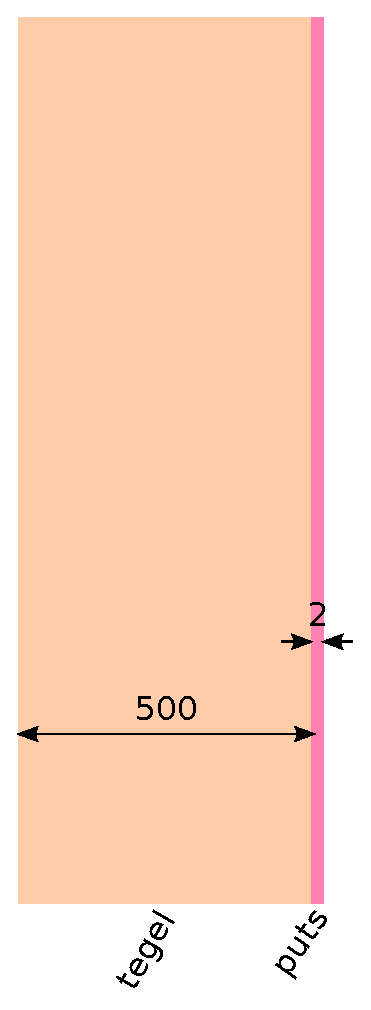
\includegraphics[height=0.3\textheight]{images/sodervagg.eps}
\caption{\label{fig:sodervagg}{Söderväggen, utifrån och in från vänster till höger. Alla mått är i mm.}}
\end{figure}

\begin{figure}[hpbt]
\centering
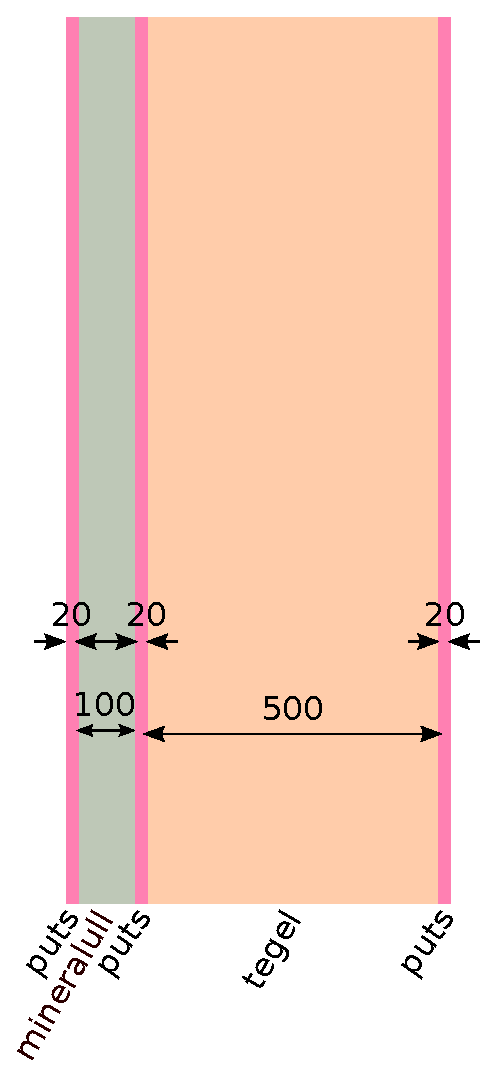
\includegraphics[height=0.3\textheight]{images/norrvagg.eps}
\caption{\label{fig:norrvagg}{Norrväggen, utifrån och in från vänster till höger. Alla mått är i mm.}}
\end{figure}

Fastigheten mellan två andra byggnader i liknande stil. Det öster om är lika högt som fastigheten medan det i väster är något lägre. Fastighetens yttervägg i väster är inte tilläggsisolerad och har samma uppbyggnad som söderväggen, se figur \ref{fig:sodervagg}.

På söderväggen finns ett burspråk som är kopparklätt kopparn sitter direkt på en cementbunden spånskiva och sedan en luftspalt om ca 2,5 cm. Väggen innanför består av 1,6 cm gips, 5 cm minneralull och sedan ytterligare 2,4 cm gips, se figur \ref{fig:bursprak}.\cite{kandidatarbete2010} Enligt Peter Särneö\cite{petersarneo} är det burspråket som läcker mest energi.

\begin{figure}[hpbt]
\centering
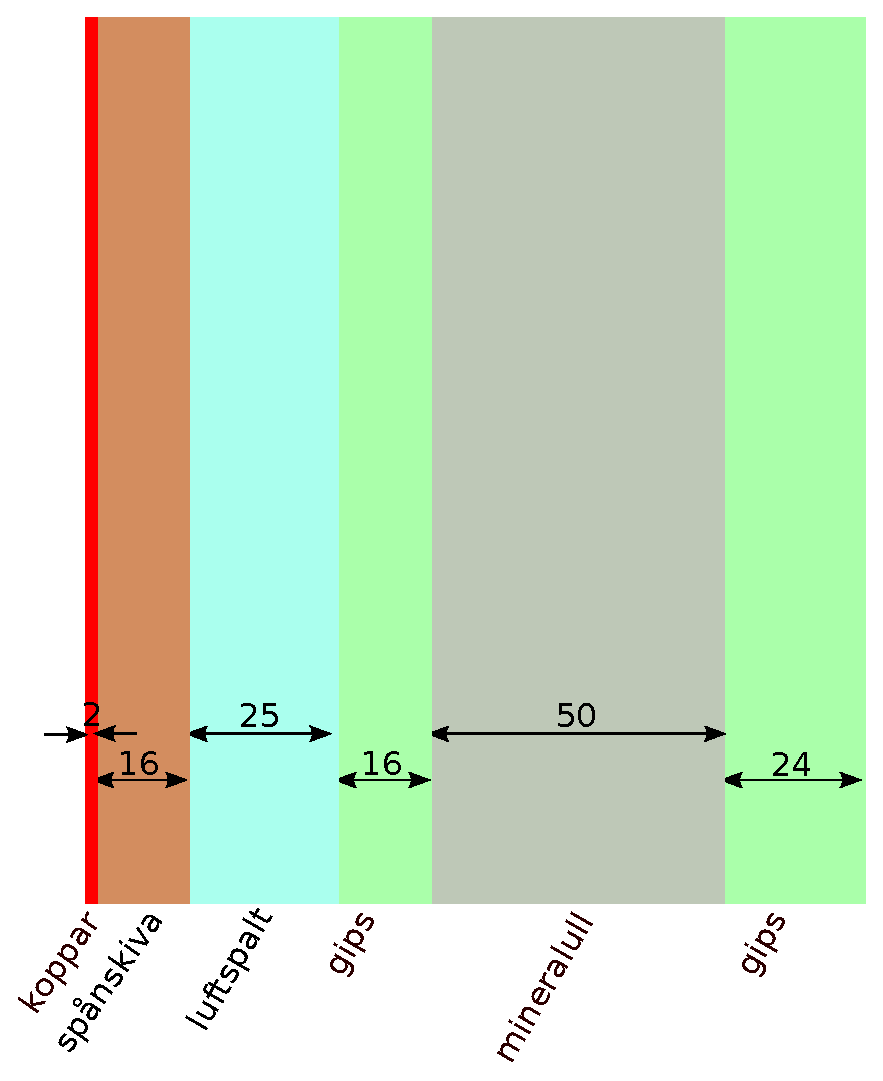
\includegraphics[width=0.3\textheight]{images/bursprak.eps}
\caption{\label{fig:bursprak}{Burspråket på söderväggen, utifrån och in från vänster till höger. Alla mått är i mm.}}
\end{figure}

\subsection{Taket}
Även taket lades om i samband med den stora renoveringen för minskad energiåtgång. Efter det bestod det av taktegel på underlagspapp ytterst, följt av 1,3 cm gips, 21 cm mineralull och innerst ytterligare 2,6 cm gips, se figur \ref{fig:taket}.\cite{kandidatarbete2010}

\begin{figure}[hpbt]
\centering
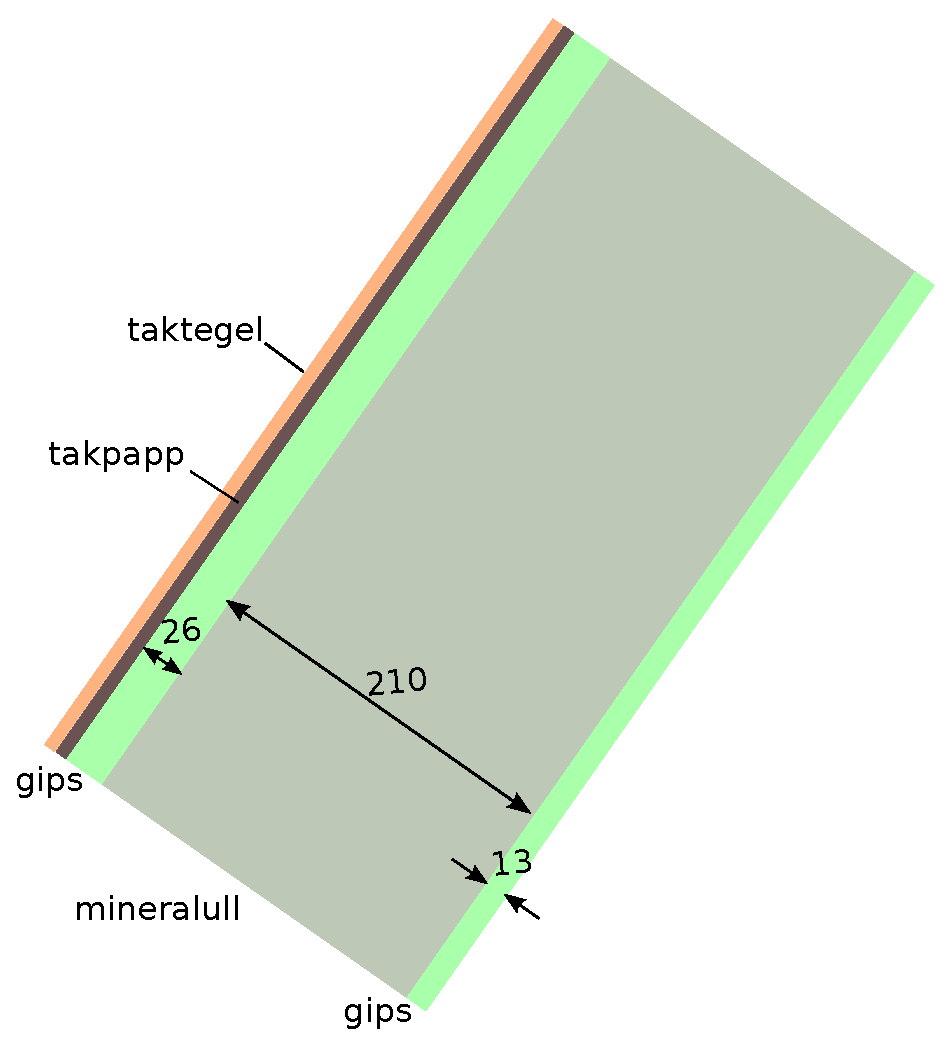
\includegraphics[width=0.3\textheight]{images/taket.eps}
\caption{\label{fig:taket}{Takets uppbyggnad. Alla mått är i mm.}}
\end{figure}

\subsection{Fönstren}

Byggnadens fönster är av treglastyp utan ytbeläggningar. Utrymmet mellan de två innersta glasskivorna är fyllt med argon för att minska värmeledningsförmågan. Totalt får fönstren ett U-värde på ungefär $\unit[1]{W/m^2}$, se avsnitt \ref{sec:heatconduction}. 

\subsection{Grunden}

Huset är byggt på ett berg som sluttar kraftigt. I östra delen av fastigheten ligger huset direkt på berget med endast ett lager av makadam emellan\cite{petersarneo}. I västra halvan har huset en undre källare, det är där apparat- och fläktrummen finns. Där är det betydligt större avstånd ned till berget, uppskattningsvis ett par meter. % Mer exakt? Källa?

\subsection{Uppvärmning och ventilation}
Idag värms huset av bergvärme från tre bergvärmepumpar. För att minska energiåtgången har ett flertal värmeväxlare installerats och värmen från all frånluft återanvänds i möjligaste mån.
% Hur fungerar regleringen? Källa?
Det är viktigt att lägenheterna är kalibrerade så att de får samma temperatur vid samma energiutflöde.

\section{Definition av väder för tillämpningar i denna rapport}
\label{subsec_weather}
Vår uppdragsgivare vill undersöka hur inomhustemperaturen påverkas av vädret. Tesen är att man kan få en mer korrekt styrning av inomhustemperaturen om man inte bara låter den påverkas av utomhustemperaturen, utan även av fler väderparamterar. Han har därför installerat en väderstation, se avnitt~ \ref{subsec_weathertransmitter}.
Begreppet väders vardagliga användningsområde är mycket brett och behöver därför avgränsas för att definiera de väderparameterar som behandlas inom projektet.

Kortfattat definieras vädret som det väderstationen tillsammans med solintensitetsmätaren mäter. Så som finns beskrivet i avsnitt~\ref{subsec_weathertransmitter} mäter vi vädret med utrustning som tar in vindens hastighet och riktning, lufttemperaturen, lufttryck, relativ fuktighet samt regn och hagels varaktighet och intensitet \cite{datasheet_weathertransmitter}. Vi kommer dock att bortse helt ifrån hagel då detta sker så sällan och i så korta perioder att det kan antas försumbart.  Dessutom mäter solintensitetsmätaren solens intensitet och varaktighet, se avsnitt~\ref{subsec:sunmeter}. % Källa på hur ofta (sällan) det haglar i Sverige. 

Tanken är att man ska kunna beskriva allt väder som en temperatur, antingen som den utomhustemperatur man bör reglera efter eller som den inomhustemperatur huset skulle få med befintlig aktivitet men utan uppvärmning, alltså ett mått på hur många grader man måste värma. Dessa två mått kallas ekvivalent temperatur och free-running temperature vilka beskrivs i avsnitt~\ref{sec:ekv_temp} respektive avsnitt~\ref{sec:freerunningtemp}. 

Från studier med hjälp av beräkningstjänsten Wolfram Alpha\cite{wolframalpha} av hur luftfuktighet kan påverkar luftens värmeledningsförmåga, får vi att den har väldigt liten betydelse. Man kan se en liten skillnad vid mycket höga luftfuktigheter (upp emot 90 \%) vid de högre temperaturerna, över $\unit[25]{^\circ C}$. Detta torde vara försumbart eftersom skillnaden är liten och endast vid väderförhållanden som inträffar relativt sällan i vårt klimat.

Hur regn och fukt påverkar fastighetensklimat har inte behandlats inom det här projektet.
Det kan dock antas att en hel del energi försvinner när väggen blir blöt och vattnet avdunstar. Troligen kyler regnet även luften.

Ytterligare en parameter som inte behandlas till är snö. När snön har lagt sig på taket kan man anta att den har en isolerande effekt. Vi kan inte mäta om och i så fall hur mycket snö det ligger på taket. Enligt SMHI\cite{SMHIdata}
rör det sig enbart om 25-50 dygn med snö i Göteborg per år. Detta påverkar dessutom främst de översta lägenheterna, de på vinden. Har man däremot en enplansvilla i Norrland kan man anta att detta är en mer betydande parameter, men det är alltså inget vi kommer att undersöka.

\subsection{Väderstationen}
\label{subsec_weathertransmitter}
I rapporten låter vi de parametrar som väderstationen tar in definiera vädret, se avnitt~\ref{subsec_weather}. Väderstationen som vår uppdragsgivare installerat är en Vaisala Weather Transmitter WXT520. Den mäter sju olika värden: vindens hastighet och riktning, lufttemperaturen, lufttrycket, den relativa fuktigheten samt regn och hagels varaktighet och intensitet. I tabell \ref{tbl:weathertransmitter} beskrivs stationens mätområde, noggrannhet och upplösning för de olika parametrarna. Vi har således väldigt liten nytta av att låta våra beräkningar vara noggrannare än väderstationen kan mäta.

\begin{table}[htdp]
\caption{Tekniska data för väderstationen, \cite{datasheet_weathertransmitter}}

\begin{center}
\begin{tabular}{|l | l l l|}
\hline
\textbf{Väder} & \textbf{Mätområde} % range
 & \textbf{Noggrannhet} % accuracy
 & \textbf{Upplösning} \\ % resolution
\hline
\rule{0pt}{3ex}Vindhastighet & $0$ -- $\unit[60]{m~s^{-1}}$ & $\pm3$ -- $5\%$ & $\unit[0,1]{m~s^{-1}}$ \\ 
\rule{0pt}{3ex}Vindriktning & alla riktningar & $\pm 3^{\circ}$ & $1^{\circ}$ \\
\rule{0pt}{3ex}Temperatur & $-52$ -- $\unit[+60]{^{\circ}C}$ & & $\unit[0,1]{^{\circ}C}$ \\
\rule{0pt}{3ex}Lufttryck & $600$ -- $\unit[1100]{hPa}$ & $0,5$ -- $\unit[1]{hPa}$ & $\unit[0,1]{hPa}$ \\
\rule{0pt}{3ex}Luftfuktighet & $0$ -- $\unit[100]{\%RH}$ & $\pm3$ -- $\unit[ 5]{\%RH}$ & $\unit[0,1]{\%RH}$ \\
\rule{0pt}{3ex}Regn &  & $\unit[5]{\%}$ & \unit[0,01]{mm} \\
~varaktighet & & & $\unit[10]{s}$\\
~intensitet & $\unit[0\mhyphen 200]{mm~h^{-1}}$ & & $\unit[0,1]{mm~h^{-1}}$ \\
\rule{0pt}{3ex}Hagel &  &  & 0,1 $\unit{cm^2}$ \\
~varaktighet & & från första träffen & 10 s\\
~intensitet & & & 0,1 $\unit{cm^{-2}~h^{-1}}$\\
\hline
\end{tabular}
\end{center}
\label{tbl:weathertransmitter}
\end{table}

\subsection{Solintensitetsmätaren}\label{subsec:sunmeter}
Mätaren för solintensitet som finns monterad på fastigheten är en Pyranometer CMP3 av märket Kipp \& Zonen. Den mäter våglängder från $300$ till $\unit[2800]{nm}$, vilket täcker in större delen av den solstrålning som når jorden. Ur databladet fås också att osäkerhet för en dag kan väntas vara under $\unit[10]{\%}$. Den största möjliga instrålningen den klarar av att mäta är $\unit[2000]{W m^{-2}}$ vilket är väl över maximala möjliga värde på jorden om man enbart mäter strålning från solen\cite{physicshandbook}. Den uppfyller gott och väl behoven för studien.\cite{datasheet_sun}




\section{En beskrivning av begreppet free-running temperature}
\label{sec:freerunningtemp}

Free-running temperature är ett begrepp som används för att sammanfatta olika 
värmeflödens påverkan på byggnader. Det finns tyvärr ingen bra svensk översättning 
men det kan beskrivas som den inomhustemperatur som fås om byggnaden används 
normalt men aktivt tillförda energin, det som normalt kallas uppvärmning via radiatorer, 
stängs av.

I en fastighet finns många olika värmekällor, så som värme från elektriska apparater, 
människorna som vistas där, belysning och varmvatten för hushållsbruk. All den värmen
 bidrar till att värma upp huset. På grund av termodynamikens huvudsatser vet vi att 
 kroppar i kontakt alltid strävar efter jämvikt och på så sätt får vi ytterligare energiflöden på 
 grund av vind, sol och utomhustemperatur.

Normalt används sedan den tillförda energin till att utjämna detta. Genom att inte värma 
fastigheten kan man istället räkna på hur mycket energi man behöver tillföra fastigheten 
vid olika tidpunkter för att nå önskad inomhustemperatur.

Denna storhet kan givetvis mätas, men eftersom man vill bibehålla aktiviteten är detta troligen inte så populärt hos de som använder byggnaden, speciellt inte med det klimat vi har i Sverige. Vi har istället valt att använda våra modeller för att beräkna den.

Måttet free-running temperature kan användas till flera olika saker. Det enklaste är att 
jämföra olika byggnader, där man i och med den fortsatt aktiviteten i byggnaden jämför
 dem med hänsyn till vad de används till – ett vilohem eller en idrottshall har troligen 
 ganska olika free-running temperature även om de skulle ha exakt samma 
 byggnadstekniska specifikation. Vid beräkning av värdet behöver man givetvis inte ta 
 hänsyn till detta men det kan ändå vara intressant för undersöka energibehovet.

Ett annat användningsområde är att sätta upp en statistisk modell där man kan visa hur 
energibehovet förändras beroende på verksamhet och väderparametrar. Detta ligger 
betydligt närmare till hands för det här arbetet och i förlängningen kanske det kan leda till 
en mer anpassat reglersystem för uppvärmningen av byggnaden.

<<<<<<< HEAD
\section*{equivalenttemperature}
Antag att det bara finns ett sorts väder, där temperaturen är den enda variabeln. Det skulle innebära att man kan hänföra hur mycket energi som går åt för att värma upp någonting direkt till utetemperaturen. Det finns oändligt antal olika vädertyper, och fler parametrar måste tas i beaktning då man räknar ut hur mycket energi som måste tillföras huset. En ekvivalent temperatur för en viss vädertyp skulle således motsvara den temperaturen, i ett optimalt klimat, som kräver tillförsel av samma energimängd för att upprätthålla efterfrågat klimat.
=======
\section*{equivalenttemperature}
Antag att det bara finns ett sorts väder, där temperaturen är den enda variabeln. Det skulle innebära att man kan hänföra hur mycket energi som går åt för att värma upp någonting direkt till utetemperaturen. Det finns oändligt antal olika vädertyper, och fler parametrar måste tas i beaktning då man räknar ut hur mycket energi som måste tillföras huset. En ekvivalent temperatur för en viss vädertyp skulle således motsvara den temperaturen, i ett optimalt klimat, som kräver tillförsel av samma energimängd för att upprätthålla efterfrågat klimat.
>>>>>>> 016a6be50697be1083f4accc334f848f4a268cd5


%Metod
\chapter{Metod}

I detta kapitel presenteras den metodik som tillämpats vid beräkning av olika energiflöden och bygger på det teoretiska underlag som presenterats i föregående kapitel. Byggnaden kommer här delas upp i de två beståndsdelarna grunden – som påverkas av vädret via med marken som värmebuffert – samt byggnadsskalet – med väggar, tak och fönster vars yta direkt påverkas av vädret. Dessutom tillkommer solinstrålningen genom fönster och ofrivillig ventilation på grund av vind, vilka betraktas helt fristående.

Vi börjar med att de analytiska beräkningar som beskriver solinstrålningen och går sedan direkt in på att beskriva hur ett statiskt värmeflöde genom en vägg kan beräknas. Vidare beskrivs hur finita elementmetoden har används för att behandla statiska flöden, som används här för att beräkna luftflödet längs väggen när det blåser.

Slutligen finns ett avsnitt som beskriver hur vi med hjälp av programmet Comsol beräknar påverkan på fastigheten från ofrivillig ventilation, det vill säga hur mycket energi som försvinner genom vind som penetrerar huset. 

\subsubsection{Solstrålning genom fönster}

För att beräkna den totala effekt solstrålning tillför byggnaden behövs fönstrenas vinkelberoende g-värden (presenterat i avsnitt \ref{gvalue}). 

För att beräkna g-värdet ur \eqref{eq:radiationwindowstheory:gvalue} behöver parametern $z = \theta/90$ beräknas, där $\theta$ är vinkeln mellan solstrålingens riktning och fönstrets normal. Detta kan göras genom att utgå från aktuellt datum och tid på dygnet.

En metod för att räkna ut solens position presenteras i \cite{walraven78} och en Matlabfunktion baserad på samma artikel kan ses i appendix. % Hänvisa till kod

Om azimuthala och altitudinella vinklarna ($\beta$ respektive $\alpha$) relativt ett väderstreck respektive horisonten tillhandahålls beräknas infallsvinkeln mot glaset, $\theta$, på följande vis:

\begin{equation} 
\theta = \frac{360}{2\pi}\arctan{\left( \sqrt{\tan^2{\left(\alpha\right)}
+ \tan^2{\left(\beta - \gamma \right)}} \right)}
\end{equation}

där $\gamma$ är vinkeln mellan fönstrets normal och väderstrecket mot vilken azimuthala vinkeln anges. Notera att alla vinklar utom $\theta$ anges i radianer.

Med dessa samband tillgängliga kan ett Matlabprogram för beräkning av effektflödet på grund av solstrålning genom fönster skapas, och ett exempel kan ses i appendix. % Hänvisa till appendix.

% Behöver: longitud, latitud, vinkeln relativt väderstreck, fönsters area, g-värde

\subsubsection{Inverkan av skuggor, gardiner och dylikt}

% Beräkna för vilka vinklar skuggor faller över fönstren

% Gardiner, persienner och interiör förändrar situationen, kolla källan nedan
\begin{comment}
Simmler & Binder
Experimental and numerical determination of the total solar energy transmittance of glazing with venetian blind shading
\end{comment}

% Be Särnöe om specifikationer:
% - I vilket väderstreck är normalen riktad?
% - Vilket g-värde har fönstren?

\begin{comment}
I diskussion:
- Hur kan man koppla detta till värmesystemet?
	- Registrera intensitet, tid på dygnet och datum
	- Beräkna ungefärlig tillförd effekt
	- Kompensera genom att säga till värmesystemet att minska/stänga inflödet
- Blir det lättare att helt enkelt mäta temperaturen i rummet och gå utifrån det? Vad är mer kostnadseffektivt?
\end{comment}

\section{Finita element av värmeledningsekvationen}
\label{sec:femheat}
I detta avsnitt behandlas finita elementlösningen av värmeledningsekvationen.
Det är från avsnitt \ref{sec:heatconduction} givet att differentialekvationen
enligt ekvation \eqref{eq:femheateq} beskriver värmeflöde i ett material.

\begin{equation}
\label{eq:femheateq}
c_p\rho\frac{\partial T}{\partial t} = \nabla\cdot(k\nabla T)
\end{equation}

\noindent
För att finna en lösning integreras värmeledningsekvationen
multiplicerat med en $L^2$ integrabel testfunktion $\phi(\mathbf{r})$ över hela
definitionsmängden $\Omega$ vars rand benämns $\Gamma$.
Detta kan ses i ekvation \eqref{eq:femheatweak}.
Nu söks en funktion $T(\mathbf{r},t)$ som satisfierar nyss nämnda uttryck för
alla $L^2$ integrabla testfunktioner $\phi(\mathbf{r})$.

\begin{equation}
\label{eq:femheatweak}
\int_\Omega \left(c_p\rho\frac{\partial T}{\partial t} -
\nabla\cdot(k\nabla T)\right)\phi(\mathbf{r})d\Omega = 0
\end{equation}

\noindent
För att förenkla fortsatta beräkningar behövers det genomföras några
omskrivningar av uttrycket. Divergensteoremet används först för att 
eliminera divergensen i värmeledningsekvationens högerled. Detta ger då
ekvation \eqref{eq:femheatweakfull}. Här är $\mathbf{n}$ normalen till randen.

\begin{equation}
\label{eq:femheatweakfull}
\int_\Omega c_p\rho\frac{\partial T}{\partial t}\phi(\mathbf{r}) +
k\nabla T\nabla\phi(\mathbf{r}) d\Omega =
\int_\Gamma k\mathbf{n}\cdot\nabla Td\Gamma
\end{equation}

\noindent
Härnäst skall galerkinformuleringen skissas. Detta genomförs
genom att temperaturen $T$ samt tidsderivatan av temperaturen $\dot{T}$
enligt ekvationerna \eqref{eq:femheatt} och \eqref{eq:femheattdot}.

\begin{align}
\label{eq:femheatt}
T(\mathbf{r}) & \approx \sum_n T_n\phi(\mathbf{r}) \\
\label{eq:femheattdot}
\dot{T}(\mathbf{r}) & \approx \sum_n \dot{T}_n\phi(\mathbf{r})
\end{align}

\noindent
Ansatsen ovan stoppas härnäst in i den svaga formuleringen i ekvation
\eqref{eq:femheatweakfull} vilket ger ekvation \eqref{eq:femheatgalerkin}.
För att kunna lösa problemet för definitionsmängder som består av olika
homogena material väljs testfunktionen $\phi$ så att den försvinner vid
alla andra material än ett och värmeledningskonstanten kan då benämnas $k_n$.
Ekvationssystemet kan sedan skrivas i matrisform vilket kan ses i ekvation
\eqref{eq:femheatmatrix}. Här är $M$ massmatrisen, $A$ är stelhetsmatrisen och
$f$ är belastningsvektorn.

\begin{align}
\label{eq:femheatgalerkin}
\sum_n \dot{T}_n \int_\Omega c_p\rho\phi_i(\mathbf{r})
\phi_n(\mathbf{r})d\Omega
& + \sum_n T_n \int_\Omega k_n \nabla\phi_n(\mathbf{r})\nabla\phi_n(\mathbf{r})
d\Omega \\
&= \int_\Gamma k_i\phi_i\mathbf{n}\cdot\nabla Td\Gamma \Leftrightarrow
\nonumber
\end{align}

\begin{equation}
\label{eq:femheatmatrix}
M\dot{T} + AT = f \Rightarrow
\end{equation}

\begin{equation}
\label{eq:femheatmatrix2}
\dot{T} + M^{-1}AT = M^{-1}f
\end{equation}

\noindent
Som kan ses så är ovanstående uttryck ett system av kopplade ordinära
differentialekvationer vars lösning är trivial med hjälp av egenvärdesuppdelning.
Vektorerna $\{v\}^n_{i=1}$ definieras som egenvektorerna av
$M^{-1}A$ och $\lambda_i$ definieras som egenvärdena till samma matris.
Systemets homogena lösning kan då skrivas som ekvation
\eqref{eq:femheathom}.\cite{lay06}

\begin{equation}
\label{eq:femheathom}
T_h(t) = \sum_n = c_nv_ne^{-\lambda_nt}
\end{equation}

\noindent
Då ekvationen är inhomogen så återstår det att lösa systemets
partikulärlösning. Då inhomogeniteten är konstant så kan lämpligen
en konstant ansättas som partikulärlösning. Detta ger att
$T_p(t) = D$. Insättning i differentialekvationen ger
ekvation \eqref{eq:femheatinstopp} vilket gör att vi kan bestämma
$D$ genom ekvation \eqref{eq:femheatinstopp2}.

\begin{align}
\label{eq:femheatinstopp}
M^{-1}AD &= M^{-1}b \Rightarrow\\
\label{eq:femheatinstopp2}
D &= A^{-1}b
\end{align}

\noindent
Nu kan den fullständiga lösningen skissas som $T = T_h + T_p$ och om
tiden sätts till noll så kan konstanterna $c_n$ bestämmas genom
att $T$ sätts till problemets begynnelsevärden. För ett problem som
saknar tidsberoende eller som har nått en jämviktspunkt måste
tiden vara oändlig och de termer som innehar exponenter blir noll.
Detta innebär att partikulärlösningen $T_p$ är den tidsoberoende lösningen
till problemet. Detta kan enkelt verifieras genom att sätta $\dot{T} = 0$.
Problemet som återstår är då $AT = b$ vars lösning är $T_p$.

\section{Värmeflöde i vägg}

För att beskriva ett värmeflöde används ekvationerna Fouriers värmeekvation
\eqref{eq:conduction:fourier} och värmeledningsekvationen 
\eqref{eq:conduction:heateq}. 
I dessa är
$k$ värmeledningsförmågan\\i $\mbox{W}\mbox{m}^{-2}\mbox{K}^{-1}$ och
$\alpha$ är termisk diffusivitet i $\mbox{m}^2\mbox{s}^{-1}$. \cite{physicshandbook}

Vid statiskt värmeflöde kommer temperaturderivatan med avseende på tiden att vara noll.
Detta innebär att värmeledningsekvationen övergår i Laplaces ekvation
$\Delta{}T = 0$. I en dimension blir detta $d^2T/dx^2 = 0$ vilket innebär
att lösningen blir ett polynom av första ordningen.  

\begin{equation}
%\label{eq:staticwallmethod:fourier}
q_x = -k \frac{dT}{dx}
\tag{\ref{eq:conduction:fourier}}
\end{equation}

\begin{equation}
%\label{eq:staticwallmethod:heat}
\frac{\partial T}{\partial t} = \alpha \Delta T
\tag{\ref{eq:conduction:heateq}}
\end{equation}

\noindent
Vi vill nu beskriva det statiska värmeflödet genom en vägg som består
av flera olika material. De enda värmekällorna som påverkar väggen
är en isoterm $T = T_H$ på ena sidan av väggen
samt en isoterm $T = T_L$ på andra sidan av väggen.

För att göra beräkningarna enklare
ser vi väggen som en oändligt stor skiva. Detta innebär att vi kan räkna
på ekvationen i en dimension. Med hjälp av det härledda sambandet i avsnitt \ref{sec:heatconduction} kan ett ekvationssystem bildas.

\begin{equation}
\label{eq:staticwalltheory:rodmatrix}
\begin{pmatrix}
Q \\
-Q
\end{pmatrix} = 
\frac{k}{L}\begin{pmatrix}
1 & -1 \\
-1 & 1
\end{pmatrix}
\begin{pmatrix}
T_1 \\
T_2
\end{pmatrix}
\end{equation}

\noindent
Vi kan nu teckna dessa ekvationssystem för alla delar av väggen, som skrivs som 
en matris och sedan fylla ut matriserna med nollelement för att slutligen bilda 
en linjärkomination.
Då linjärkombinationen bildas kommer energiflödena i mitten av väggen att
vara noll. Detta överensstämmer väl med att vi har en statisk energifördelning
utan interna värmekällor.
Slutligen får vi ett ekvationsystem enligt ekvation
\eqref{eq:staticwallmethod:full} som enkelt kan lösas.
Matrisen $A$ är linjärkombinationen av nollutfyllda versioner av matrisen i ekvation
\eqref{eq:staticwalltheory:rodmatrix} enligt ekvation
\eqref{eq:staticwallmethod:example}.

\begin{equation}
\label{eq:staticwallmethod:example}
A = \frac{k_1}{L_1}
\begin{pmatrix}
1 & -1 & 0 &  \dots \\
-1 & 1 & 0 &   \\
0 & 0 & 0 &  \\
\vdots & & & \ddots
\end{pmatrix}
+
\frac{k_2}{L_2}
\begin{pmatrix}
0 & 0 & 0 & 0 & \dots \\
0 & 1 & -1 & 0 &  \\
0 & -1 & 1 & 0 & \\
0 & 0 & 0 & 0 & \\
\vdots & & & & \ddots
\end{pmatrix} + \dots
\end{equation}

\begin{equation}
\label{eq:staticwallmethod:full}
\begin{pmatrix}
Q\\0\\...\\0\\-Q
\end{pmatrix} = A
\begin{pmatrix}
T_H\\T_1\\...\\T_{n-1}\\T_L
\end{pmatrix}
\end{equation}

Här gör vi en jämförelse mellan en oisolerad, 50 cm tjock tegelvägg, motsvarande den som finns på fastighetens södersida, och en 50 cm tjock tegelvägg med 10 cm isolering, motsvarande den som finns på fastighetens norrsida.

\section{Finita element av värmeledningsekvationen}
\label{sec:femheat}
I detta avsnitt behandlas finita elementlösningen av värmeledningsekvationen.
Det är från avsnitt \ref{sec:heatconduction} givet att differentialekvationen
enligt ekvation \eqref{eq:femheateq} beskriver värmeflöde i ett material.

\begin{equation}
\label{eq:femheateq}
c_p\rho\frac{\partial T}{\partial t} = \nabla\cdot(k\nabla T)
\end{equation}

\noindent
För att finna en lösning integreras värmeledningsekvationen
multiplicerat med en $L^2$ integrabel testfunktion $\phi(\mathbf{r})$ över hela
definitionsmängden $\Omega$ vars rand benämns $\Gamma$.
Detta kan ses i ekvation \eqref{eq:femheatweak}.
Nu söks en funktion $T(\mathbf{r},t)$ som satisfierar nyss nämnda uttryck för
alla $L^2$ integrabla testfunktioner $\phi(\mathbf{r})$.

\begin{equation}
\label{eq:femheatweak}
\int_\Omega \left(c_p\rho\frac{\partial T}{\partial t} -
\nabla\cdot(k\nabla T)\right)\phi(\mathbf{r})d\Omega = 0
\end{equation}

\noindent
För att förenkla fortsatta beräkningar behövers det genomföras några
omskrivningar av uttrycket. Divergensteoremet används först för att 
eliminera divergensen i värmeledningsekvationens högerled. Detta ger då
ekvation \eqref{eq:femheatweakfull}. Här är $\mathbf{n}$ normalen till randen.

\begin{equation}
\label{eq:femheatweakfull}
\int_\Omega c_p\rho\frac{\partial T}{\partial t}\phi(\mathbf{r}) +
k\nabla T\nabla\phi(\mathbf{r}) d\Omega =
\int_\Gamma k\mathbf{n}\cdot\nabla Td\Gamma
\end{equation}

\noindent
Härnäst skall galerkinformuleringen skissas. Detta genomförs
genom att temperaturen $T$ samt tidsderivatan av temperaturen $\dot{T}$
enligt ekvationerna \eqref{eq:femheatt} och \eqref{eq:femheattdot}.

\begin{align}
\label{eq:femheatt}
T(\mathbf{r}) & \approx \sum_n T_n\phi(\mathbf{r}) \\
\label{eq:femheattdot}
\dot{T}(\mathbf{r}) & \approx \sum_n \dot{T}_n\phi(\mathbf{r})
\end{align}

\noindent
Ansatsen ovan stoppas härnäst in i den svaga formuleringen i ekvation
\eqref{eq:femheatweakfull} vilket ger ekvation \eqref{eq:femheatgalerkin}.
För att kunna lösa problemet för definitionsmängder som består av olika
homogena material väljs testfunktionen $\phi$ så att den försvinner vid
alla andra material än ett och värmeledningskonstanten kan då benämnas $k_n$.
Ekvationssystemet kan sedan skrivas i matrisform vilket kan ses i ekvation
\eqref{eq:femheatmatrix}. Här är $M$ massmatrisen, $A$ är stelhetsmatrisen och
$f$ är belastningsvektorn.

\begin{align}
\label{eq:femheatgalerkin}
\sum_n \dot{T}_n \int_\Omega c_p\rho\phi_i(\mathbf{r})
\phi_n(\mathbf{r})d\Omega
& + \sum_n T_n \int_\Omega k_n \nabla\phi_n(\mathbf{r})\nabla\phi_n(\mathbf{r})
d\Omega \\
&= \int_\Gamma k_i\phi_i\mathbf{n}\cdot\nabla Td\Gamma \Leftrightarrow
\nonumber
\end{align}

\begin{equation}
\label{eq:femheatmatrix}
M\dot{T} + AT = f \Rightarrow
\end{equation}

\begin{equation}
\label{eq:femheatmatrix2}
\dot{T} + M^{-1}AT = M^{-1}f
\end{equation}

\noindent
Som kan ses så är ovanstående uttryck ett system av kopplade ordinära
differentialekvationer vars lösning är trivial med hjälp av egenvärdesuppdelning.
Vektorerna $\{v\}^n_{i=1}$ definieras som egenvektorerna av
$M^{-1}A$ och $\lambda_i$ definieras som egenvärdena till samma matris.
Systemets homogena lösning kan då skrivas som ekvation
\eqref{eq:femheathom}.\cite{lay06}

\begin{equation}
\label{eq:femheathom}
T_h(t) = \sum_n = c_nv_ne^{-\lambda_nt}
\end{equation}

\noindent
Då ekvationen är inhomogen så återstår det att lösa systemets
partikulärlösning. Då inhomogeniteten är konstant så kan lämpligen
en konstant ansättas som partikulärlösning. Detta ger att
$T_p(t) = D$. Insättning i differentialekvationen ger
ekvation \eqref{eq:femheatinstopp} vilket gör att vi kan bestämma
$D$ genom ekvation \eqref{eq:femheatinstopp2}.

\begin{align}
\label{eq:femheatinstopp}
M^{-1}AD &= M^{-1}b \Rightarrow\\
\label{eq:femheatinstopp2}
D &= A^{-1}b
\end{align}

\noindent
Nu kan den fullständiga lösningen skissas som $T = T_h + T_p$ och om
tiden sätts till noll så kan konstanterna $c_n$ bestämmas genom
att $T$ sätts till problemets begynnelsevärden. För ett problem som
saknar tidsberoende eller som har nått en jämviktspunkt måste
tiden vara oändlig och de termer som innehar exponenter blir noll.
Detta innebär att partikulärlösningen $T_p$ är den tidsoberoende lösningen
till problemet. Detta kan enkelt verifieras genom att sätta $\dot{T} = 0$.
Problemet som återstår är då $AT = b$ vars lösning är $T_p$.


\section{Värmeflöde genom grunden}

För att räkna på energin som flödar genom grunden är det nödvämdigt att räkna
transient. Detta då berget tar åt sig värme väldigt långsamt. I praktien innebär detta att ett statiskt jämviktsläge aldrig uppnås.

Problemet är behandlat med finita elementmetoden av värmeledningsekvationen.
Geometrin av problemet och trianguleringen kan ses i figur \ref{fig:foundation:tri}.
Randvärdena som är satt är att alla rander som går från berg till berg är adiabatiska.
Detta kommer inte stämma i praktiken om inte definitionsmängden sätts till oändligt
stor. För lösning av detta problem kan det dock ses som en tillräckligt god
approximation eftersom definitionsmängden är stor och temperaturen inte varierar så mycket
från förväntat värde.

Vid randerna mot grunden ligger ett neumannvillkor som säger att energiflödet är produkten
av temperaturdifferansen mellan temperaturen på randen och inomhustemperaturen på $\unit[20]{^\circ C}$.
Grundens U-värde har här satts till $U = 0,7/0,45 \approx \unit[1,556]{ Wm^{-2}K^{-1}}$. Detta värde är
baserat på att det ligger $\unit[0,25]{m}$ betong mellan källaren och grunden och att det ligger ytterligare $\unit[0,2]{m}$
betong mellan uppvärmda utrymmen och källaren. Vidare antas att det föreligger god omrörning i de båda
luftskikten vilket gör att de har $R=0$. Detta antagande är dock inte helt giltigt vilket leder till att kyleffekten
uppskattas vara något för hög.
Vid randerna till luft är konvektionsparametern satt
till $h = \unit[15,5]{Wm^{-2}K^{-1}}$. Detta är en siffra som motsvarar
en vindhastighet på ungefär $v = \unit[2]{ms^{-1}}$. Utomhustemperaturen har valts
som en minstakvadratanpassad trigonetrisk funktion av
medeltemperaturen de senaste tjugo åren vilket kan ses i figur
\ref{fig:foundation:meantemperature}. Anpassningen gör att
differentialekvationerna av galerkinformuleringen kan lösas analytiskt
för alla tider istället för att systemet ska behöva lösas semidiskret.
Detta minskade exekveringstiden dramatiskt vilket gav möjlighet att använda en
mycket finare triangulering. Dessutom kan alla termer i lösningen
som går mot noll då tiden går mot oändligeheten sättas till noll. Detta innebär
att få lösningar når ett transient jämviktsläge som liknar det jämviktsläge vi har i praktiken.
Initialvärdena kommer således inte ha någon betydelse och dessa kan då väljas
godtyckligt. 
För att uppnå detta resultat med semidiskret MOL behövs väldigt många itereringar för att
nå konvergens. Den resulterande koden kan ses i bilaga \ref{app:femfoundation}.

\begin{figure}
\centering
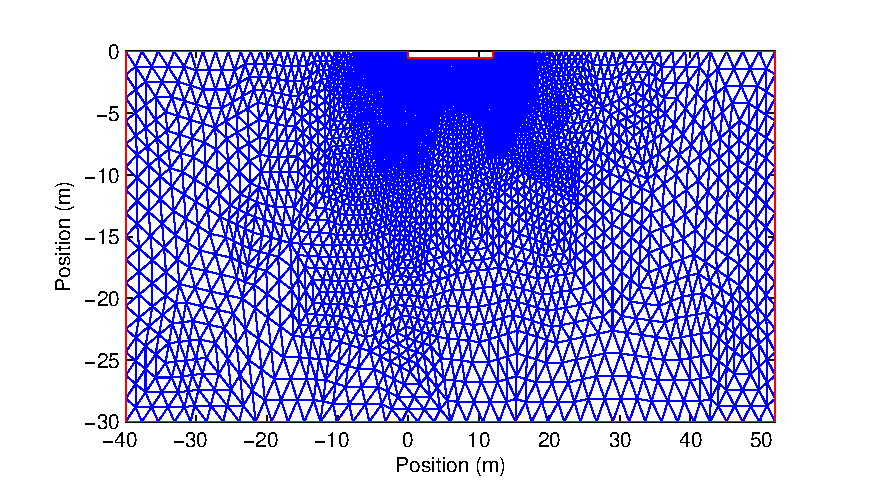
\includegraphics{images/trifoundation.eps}
\caption{Definitionsmängd och triangulering berget under grunden.}
\label{fig:foundation:tri}
\end{figure}


\begin{figure}
\centering
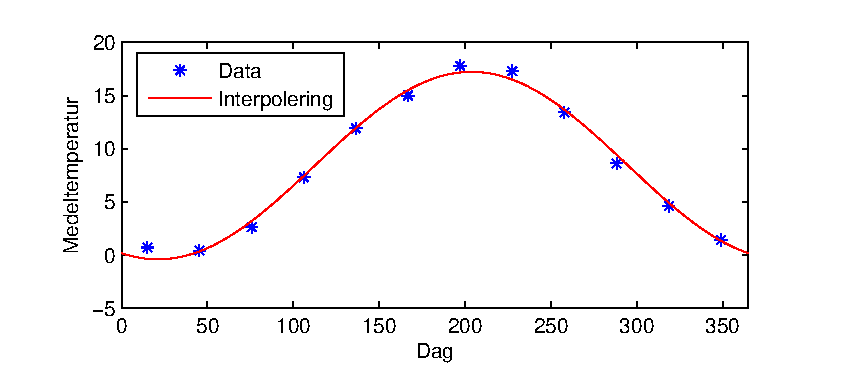
\includegraphics{images/meantemperature.eps}
\caption{
Medeltemperaturen för Göteborg de senaste 20 åren. Punkterna är data tagna från Miljöförvaltningen och linjen är minstakvadratanpassningen som senare använts för att beräkna energiflöden.}
\label{fig:foundation:meantemperature}
\end{figure}

%Miljöförvaltningen
%http://www4.goteborg.se/prod%5Csk%5Cstatistik%5CstatistikR5.nsf/0/3F002A395ED39AC8C1256D3B00393D0E/$File/3.01.pdf

\subsection{Finita element av inkompressibel fluid}

För att lösa Navier-Stokes ekvationer kan lämpligen en datormodell användas.
Här består denna modell av ett system uppsatt med Galerkins metod.
I denna lösning så begränsar vi dock oss till att enbart behandla statiska flöden
vilket genomförs genom att sätta alla tidsderivator till noll.

För att hantera trycket i \eqref{eq:convection:continuity}-\eqref{eq:convection:energy} används den tidigare nämnda Boussinesq approximation
samt penalty metoden för att göra hastighetsvektorn källfri och uppfylla
kontinuitetsekvationen. Det finns således inget direkt behov av att räkna ut trycket.
Vid användning av många sorters elementtyper som inte uppfyller Babuska-Brezzikriteriet
är detta dessutom nödvändigt då det annars kan bildas oönskade trycknoder. 
En annan möjlighet är att välja divergensfria element. \cite{babuska1973}\cite{segal2011}

Genom penaltymetoden beskrives här trycket som $p$ enligt ekvation
\eqref{eq:femconvection:penalty}. Här är $p_s$ någon form av idealt statiskt
tryck som är önskat. Detta tryck följer Boussinesq approximation. Med dessa
idealiseringar kan differentialekvationerna sättas upp igen. \cite{heinrich88}\cite{taylor79}
Som kan ses så leder den godtyckliga penaltyparametern $\lambda$ till att justera trycket
om hastighetsfältets divergens ej är identiskt noll. I viss litteratur anges 
det att penaltyparametern skall vara i storleksordningen $10^7$ men att den
är väldigt applikationsberoende. En för liten vald penaltyparameter leder till att
trycket inte elimineras. Andra problem uppstår vid en för stor parameter. Ekvationssystemet
kan bli svårlöst och få stabilitetsproblem när parametern blir
för stor i jämförelse med de andra delarna i differentialekvationen.\cite{reddy93}\cite{roy05}\cite{basak04}\cite{segal2011}

\begin{equation}
\label{eq:femconvection:penalty}
p = p_s - \lambda\nabla\cdot\mathbf{v}
\end{equation}

\noindent
Fortsatt skall trycket deriveras med avseende på de rumsliga variablerna vilket möjliggör
att eliminera trycket från differentialekvationerna. Dessa deriveringar kan ses i ekvation
\eqref{eq:femconvection:partx} samt \eqref{eq:femconvection:partz}. Notera att det statiska trycket
$p_s$ ej beror på $x$ vilket resulterar i att derivatan är noll.

\begin{equation}
\label{eq:femconvection:partx}
\frac{\partial p}{\partial x} = \frac{\partial p_s}{\partial x} -
\frac{\partial}{\partial x} \lambda\nabla\cdot\mathbf{v} = -
\frac{\partial}{\partial x} \lambda\nabla\cdot\mathbf{v}
\end{equation}

\begin{equation}
\label{eq:femconvection:partz}
\frac{\partial p}{\partial z} = \frac{\partial p_s}{\partial z} -
\frac{\partial}{\partial z} \lambda\nabla\cdot\mathbf{v} =
-g\rho_0 - \frac{\partial}{\partial z} \lambda\nabla\cdot\mathbf{v}
\end{equation}

\noindent
Detta förs in i momentekvationerna vilket ger ekvationerna \eqref{eq:femconvection:u} -
\eqref{eq:femconvection:T}. Här är det ekvationssystem som syftar att lösas.

\begin{equation}
\label{eq:femconvection:u}
\mathbf{v}\cdot\nabla u =
\frac{\lambda}{\rho_0}\nabla\cdot\mathbf{v} +
\nu\Delta u
\end{equation}

\begin{equation}
\label{eq:femconvection:w}
\mathbf{v}\cdot\nabla w =
\frac{\lambda}{\rho_0}\nabla\cdot\mathbf{v} + \nu\Delta w +g\beta(T-T_0)
\end{equation}

\begin{equation}
\label{eq:femconvection:T}
\mathbf{v}\cdot\nabla T = \alpha\Delta T
\end{equation}

\subsubsection{Svag formulering}

En finita elementlösning med Galerkins metod kräver att problemet reduceras till
ett ekvivalent variationsproblem. Här söks $T\in\Phi$, $u\in\Phi$ och
$w\in\Phi$ som uppfyller ekvation \eqref{eq:femconvection:variation}. Här
betecknar brackets skalärprodukt, $\mathbf{L}$ är differentialoperatorn
som betecknar systemet av differentialekvationer som $\mathbf{L}(T,u,w) = 0$.
$\Phi$ är rummet av alla testfunktioner $\phi$ som är kontinuerliga i
definitionsmängden $\Omega$ samt vars derivator är bitvis kontinuerliga på randen
$/Gamma$. De måste även vara $L^2$ integrabla.

\begin{equation*}
\label{eq:femconvection:variation}
\langle \mathbf{L}(T,u,w), \phi \rangle = 0\mbox{,  } \forall \phi \in \Phi
\end{equation*}


\section{Datorsimulering av ofrivillig ventilation}

Ett hus är i praktiken omöjligt att göra helt tätt. Då vinden ligger på
får man därför ett drag genom huset, en ofrivillig ventilation. Då vinden
sällan är lika varm som inomhusluften leder detta till en energiförlust.
Den har beräknats med hjälp av programvaran Comsol. Problemets geometri har
setts upp enligt figur~ \ref{fig:windmethod:tri}. Bredvid fastigheten på Walleriusgatan ligger en annan byggnad och problemet med vind från de olika hållen blir symmetriskt. Blåser det från norr illustreras den för projektet aktuella fastigheten till höger i bild, och blåser det från söder påverkas den som den till vänster.

Från vänstra kanten så har luften blåst in med en konstant vindhastiget som varieras mellan olika
experiment. På andra sidan av fastigheterna har det satt ett konstant lufttryck som motsvarar en
atmosfärs tryck. På randerna som ligger mot mark eller mot hus är vindhastigheten satt till noll.
Slutligen utför ej luftmassan ovanför definitionsmängden någon kraft på luften som ligger längs den
övre randen.

\begin{figure}
\centering
\includegraphics[width=127mm,height=76mm]{images/triinfiltration.eps}
\caption{Triangulering samt definitionsmängd uppsatt för problemet.}\label{fig:windmethod:tri}
\end{figure}

Trycket inne i fastigheterna har sedan beräknats genom att luftläckaget antagits homogent utspritt över fastigheternas
väggar och att inget luft läckt genom taket. Därefter har Darcys lag satts upp med antagande om jämvikt så att lika mycket
luft som flödar in även kommer ut. Då både trycket inomhus och på ränderna är kända kan läckaget beräknas med Darcys lag
eller med någon annan exponent, se avsnitt~\ref{sec:darcy}. Här är antagandet gjort att huset läcker mycket och har $C(50)^{0,60} = 1,2$. \emph{\color{red} Vad menas här? Vad kom C ifrån? och siffrorna?} Dock kommer även exponenten ha betydelse för läckaget.\cite{sasic}



%Resultat
\chapter{Resultat}

I detta kapitel presenteras de resultat som erhållts med hjälp av metodiken i föregående kapitel. De olika delresultaten visar på olika typer av energiflödens karaktär och hur de påverkas av väderparametrarna. Kapitlet avslutas med sammanställning av de individuella bidragen i from av totalt energiflöde genom fastigheten.

Genom att beräkna storlekarna av energiflödena genom byggnadens olika delar är det möjligt att identifiera var energiflödena är som störst vid olika väderförhållanden. För att få en uppfattning om hur det ser ut visas en klar och en molnig dag i mitten av april som får representera ett tänkt maximum för varmt väder innan eldningssäsongen tar slut. Dessutom visas en klar och en molnig dag i december som representerar ett tänkt minimum för största möjliga energiutflöde ur fastigheten, mitt under eldningssäsongen. Eldningssäsongen, det vill säga den tid på året då man fortfarande värmer upp huset, sträcker sig ungefär från början oktober till slutet av april för fastigheten på Walleriusgatan. Under sommaren sker ingen uppvärmning.

Under aprildagen når solinstrålningen en topp vid $\unit[640]{W/m^2}$ och solen är uppe i 14 timmar. Dygnets temperatur varierar mellan $\unit[6]{^\circ C}$ och $\unit[9]{^\circ C}$. Enligt väderstatistik från SMHI\cite{SMHIdata} bör detta vara en rimlig dag med väldigt bra väder vid den valda tiden på året. På samma sätt är decemberdagen vald med en temperaturvariation mellan $-11$ och $\unit[-5]{^\circ C}$ och solen når ett instrålningsmaximum på $\unit[300]{W/m^2}$.

\section{Kvantifiering av konstanta energiflöden}

Flera av energiflödena genom fastigheten är relativt konstanta sett till en längre tidsperiod. Det gäller främst värme från elektriska apparater, så som kylskåp och datorer, människors kroppsvärme och varmvattencirkulation. På så sätt kan aktivt tillförd energi, det vill säga den energitillförsel som kan regleras och tillförs via radiatorerna, enkelt regleras med hänsyn till dessa, om man bara känner dess storlek.

\subsection{Uppvärmning från människor}
Den utstrålade kroppsvärmen från människor kan beräknas genom att de antas vara svartkroppar. Stefan-Boltzmanns lag säger då att utstrålade energi per yt- och tidsenhet är $j=\sigma T^4$, där $T$ är temperaturen och $\sigma=\unit[5.6705\cdot 10^8]{Wm^{-2}K^{-4}}$ \cite{physicshandbook}, se teoriavsnitt \ref{sec:blackbody}. På samma sätt beräknas den energi som strålas in mot kroppen från omgivningen. Nettostrålningen från en människa kan då ses i ekvation \eqref{eq:constantsources:stefan} där $T_k=37^{\circ}C=310K$ är kroppstemperaturen och $T_r=20^{\circ}C=293K$ är rumstemperaturen. Multipliceras det med en människas area, ungefär $\unit[2]{m^2}$, fås en nettoeffekt på $\unit[211]{W}$. I själva verket reduceras denna effekt av en rad faktorer. Exempelvis är hudens temperatur lägre än kroppstemperaturen samtidigt som klädesplagg reducerar effektutstrålningen något. Professor Göran Grimvall skriver i NyTeknik att en rimlig nettoeffekt vid vila är cirka 1 W per kilogram kroppsvikt, alltså ungefär $\unit[50-100]{W}$\cite{Grimvall}.

\begin{equation}
\label{eq:constantsources:stefan}
j=\sigma \left( T_k^4 - T_r^4 \right)
\end{equation}
\noindent

\subsection{Varmvattencirkulation i fastigheten}
I huset cirkulerar hela tiden varmvattnet för att alltid kunna tillgodose de boendes behov av varmvatten utan dröjsmål. Efter en tur i systemet sjunker temperaturen på varmvattnet med tre grader och flödet är $\unit[800]{l/h}$. Detta motsvarar en energitillförsel till fastigheten på $\unit[2,8]{kW}$.

\subsection{Energi från elektrisk apparatur}
Den största delen av energin som driver en elektrisk apparat blir till värme. Därför låter vi energiflödet från elektriska apparatur motsvaras av fastighetens energiförbrukning, vilken kan läsas av kontinuerligt och på så sätt bli en del av reglersystemet.



\subsection{Energiflöde genom väggar}

Hur värmen sprider, eller inte sprider, sig genom en vägg beror på dess material och temperaturerna på vardera sidan av väggen. I fallet när ena sidan av väggen befinner sig utomhus beror spridning också av solinstrålningen och hur mycket det blåser från olika håll. För detta har en modell satts upp utifrån vilken det har gjorts beräkningar av storleken på energiflödet genom väggen under ett dygn då mängden moln är konstant. En modell för hur energiflödet skulle förändras vid ett väderomslag har också satts upp. Båda modellerna har sedan används för både en oisolerad vägg bestående enbart av 50 cm tegel och en vägg isolerad med 10 cm mineralull.

Slutligen har det gjorts beräkningar på hur stora tryckskillander en vind som är ortogonal mot väggen ger upphov till. Dessa tryckförändringar driver luft att färdas genom otätheter i huset och drag uppstår vilket ger ett energiflöde genom väggen vid olika inom- och utomhustemperaturer.

\subsection{Flöde vid termisk jämvikt}
\label{sec:steadystatewall}

%To regerenate the figures use /code/pdesolver/generateWallFigApril.m
%with the argument /code/pdesolver/walldata.mat

För att visualisera flödet genom en vägg vid konstant väder och utomhustemperatur görs 
beräkningar med finita elementmetoden och en konstant inomhustemperatur på 
$\unit[20]{^\circ C}$. Utomhusvädret är relativt konstant och är satt till antingen molnig 
eller klart en dag i april då utomhustemperaturen varierar mellan $\unit[6]{^\circ C}$ på natten och $\unit[9]{^\circ C}$ på dagen. Detta har gjorts för en vägg utan isolering och en vägg med 
isolering, se figur~\ref{fig:energyflow_stst}. Den oisolerade väggen består av 
$\unit[0,5]{m}$ tegel och den isolerade har dessutom $\unit[0,1]{m}$ mineralull. 

\begin{figure}[hpbt]
\centering

\subfloat[Energiflöde ut från insidan av en oisolerad vägg en klar dag i april.]{
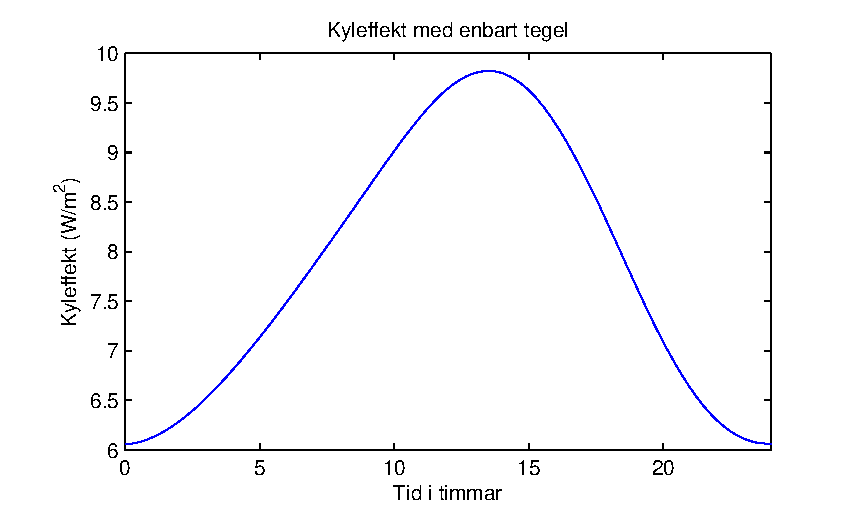
\includegraphics[width=6cm]{images/noinsulationapril.eps}}\vspace{1cm}
\subfloat[Energiflöde ut från insidan av en isolerad vägg en klar dag i april.]{
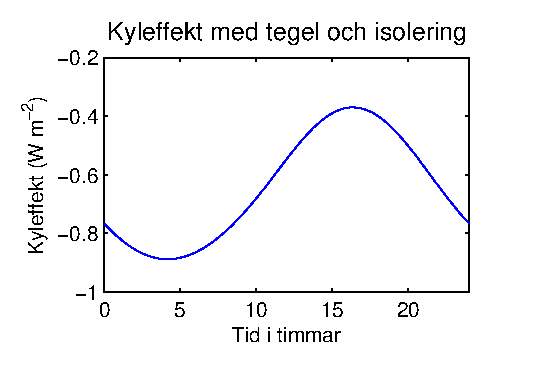
\includegraphics[width=6cm]{images/insulationapril.eps}
}

\subfloat[Energiflöde ut från insidan av en oisolerad vägg en molnig dag i april.]{
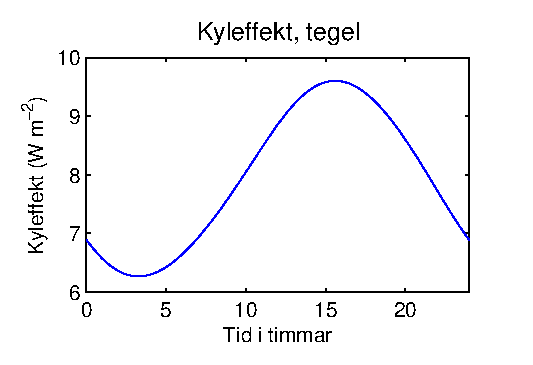
\includegraphics[width=6cm]{images/noinsulationcloud.eps}}\vspace{1cm}
\subfloat[Energiflöde ut från insidan av en isolerad vägg en molnig dag i april.]{
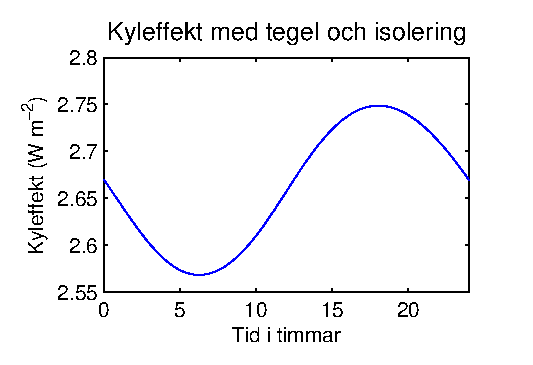
\includegraphics[width=6cm]{images/insulationcloud.eps}
}

\caption{\label{fig:energyflow_stst} Energiflöden ut från insidan av en vägg en dag i mitten av april. Utflöden ut genom väggen betecknas positivt, och inflöden negativt. }
\end{figure}


%RESULTAT ur graferna 
I figur \ref{fig:energyflow_stst} kan vi se att energiflödet genom väggen minskar till 
ungefär en fjärdedel med isolering. Under ett soligt dygn kommer det att flöda värme in i
 fastigheten. På grund av fördröjningen i väggen sker detta främst under natten, 
 och mindre på dagen. Med isolering blir energiflöde mindre och jämnare och inflödet når aldrig över $\unit[1]{W~m^{-2}}$.

Under en molnig dag med samma temperatur varierar energiflödet mellan $6$ och $10$ 
$\unit{W~m^{-2}}$ utan isolering. Med isolering minskar det till att röra sig mellan $1,9$ och $2,2$ $\unit{W~m^{-2}}$ ut ur 
fastigheten. En isolering innebär en molnig aprildag ett minskat energiutflöde och därmed en minskad 
energiförlust för fastigheten.

Trots att energi flödar in i fastigheten den klara dygnet så flödar ganska mycket energi 
ut ur fastigheten under det molniga dygnet. Göteborg har 1800 soltimmar under ett
 år av de totalt 4380 timmar som solen är över horisonten. Utifrån SMHI:s väderstatistik \cite{SMHIdata}
 kan beräknas att ungefär 37\% av dessa sker under eldningssäsongen, oktober till april. 
 Detta motsvarar ungefär 8\% av dygnets alla timmar. Tyvärr så förlorar fastigheten mer 
 energi än vad den tjänar på att inte isoleras utslaget på hela eldningssäsongen.

Under en fin sommardag kan det också tänkas att fastigheten värms över den önskade 
temperaturen och energi istället måste läggas på kylning. Med en isolering minskas även 
effekten av detta och energiflödena blir mindre och jämnare.

%%%%%%%%%%%%%%%%%%%%%%%%%%%%%%%%%%%%%%%%%%%%
\paragraph{En decemberdag}

Vidare har också energiflödena genom väggen en kall decemberdag undersökts, 
alltså en dag där energiflödena bör bli ganska stora. Detta kan ses som en övre uppskattning på fastighetens energiåtgång. Två fall av
denna dag har undersökts, dels en molning dag och dels en klar dag.

 Temperaturen går från $\unit[-5]{^\circ C}$ på dagen till $\unit[-11]{^\circ C}$. 
 Konvektionskoefficienten har satts till $h=\unit[35]{W~m^{-2}~K^{-1}}$ 
 vilket motsvarar en vindhastighet $\unit[7]{m~s^{-1}}$ parallellt med väggens yta. 
 Beräkningarna är genomförda genom att väggens tvärsnitt approximerats med en stav och sedan behandlats med finita elementmetoden.


\begin{figure}[hpbt]
\centering
\subfloat[Energiflöde ut från insidan av en oisolerad vägg en molnig dag i december.]{
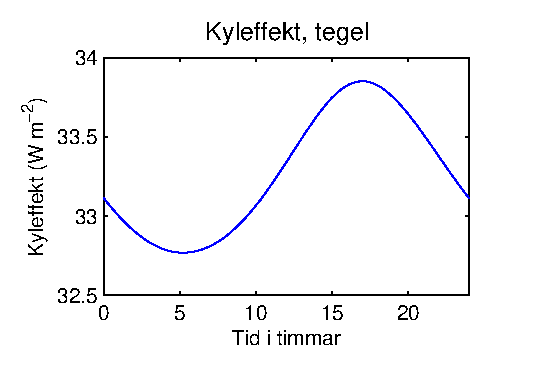
\includegraphics[width=6cm]{images/noinsulationdec.eps}}
\subfloat[Energiflöde ut från insidan av en isolerad vägg en molnig dag i december..]{
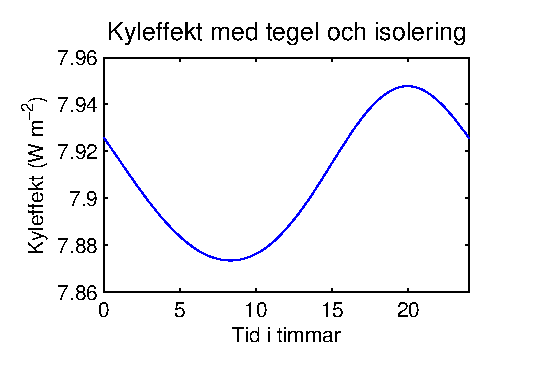
\includegraphics[width=6cm]{images/insulationdec.eps}
}

\subfloat[Energiflöde ut från insidan av en oisolerad vägg en klar dag i december.]{
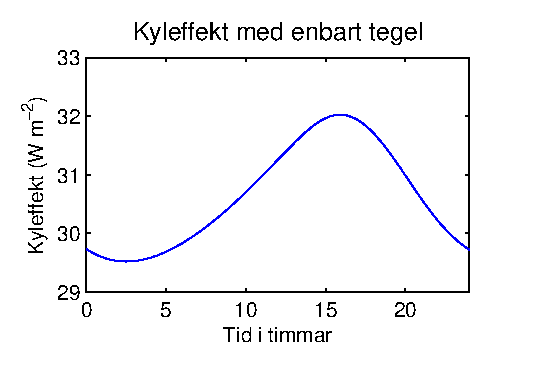
\includegraphics[width=6cm]{images/decsunnoinsulation.eps}
}\vspace{1cm}
\subfloat[Energiflöde ut från insidan av en isolerad vägg en klar dag i december.]{
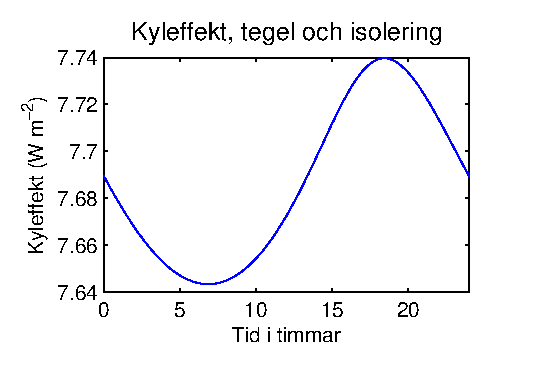
\includegraphics[width=6cm]{images/decsuninsulation.eps}
}

\caption{\label{fig:wall_dec} Energiflöden ut från insidan av en vägg en dag i december Utflöden ut genom väggen betecknas positivt, och inflöden negativt. 
}
\end{figure}

% Resultat
Även i december blir energiflödet genom en isolerad vägg ungefär en fjärdedel av det 
genom en oisolerad vägg, se figur~\ref{fig:wall_dec}. Här minskar det dock från ungefär $33,5$ 
till $\unit[8,05]{W~m^{-2}}$ ut ur väggen för den molniga dagen och från ungefär $32$ till $7,7$ $\unit{W~m^{-2}}$ den soliga dagen. Vi ser också i figurerna att energiflödet också blir 
jämnare med isolering – det varierar med mindre än $\unit[0,1]{W~m^{-2}}$ över dygnet, 
istället för drygt $\unit[1]{W~m^{-2}}$ utan isolering. Det gäller både vid klart och mulet väder. Detta är eftersträvansvärt om en jämn inomhustemperatur önskas. Energiflödet påverkas inte lika mycket av solen på vintern som under den varmare delen av året. En dag i december finns det betydligt mindre att tjäna på att inte isolera och hoppas att solen skiner, jämfört med en dag i april.

%%%% BURSPRÅK %%%%%%%%%%%%%%%%%%%%%%%%%%%%%%%
\paragraph{Burspråket}

Burspråket är inte uppbyggt av tegel, som de andra väggarna, utan av gips, isolering och koppar på spånskiva, se avsnitt~\ref{subsec:walls}. Energiflödet i burspråket visas här för alla fyra fallen: klar och molnig aprildag samt klar och molnig decemberdag.

\begin{figure}[hpbt]
\centering
\subfloat[\label{fig:bursprak_april1} Energiflöde ut från insidan av burspråket en klar dag i april.]{
	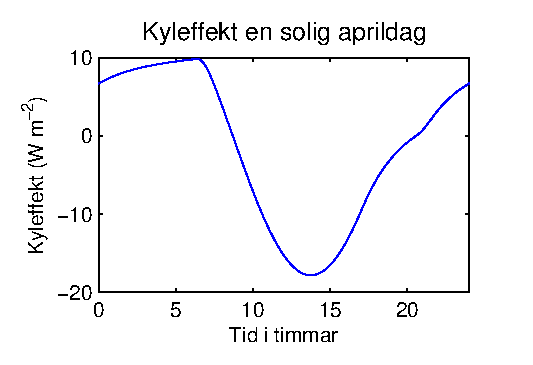
\includegraphics[width=6cm]{images/baysunapril.eps}
}
\subfloat[\label{fig:bursprak_april2} Energiflöde ut från insidan av burspråket en molnig dag i april.]{
	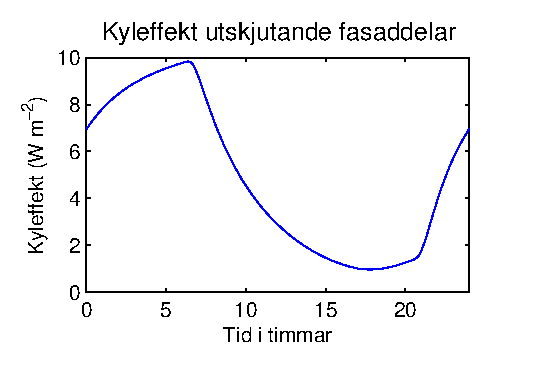
\includegraphics[width=6cm]{images/baynosunapril.eps}
}

\subfloat[\label{fig:bursprak_decsun} Energiflöde ut från insidan av burspråket en klar dag i december.]{
  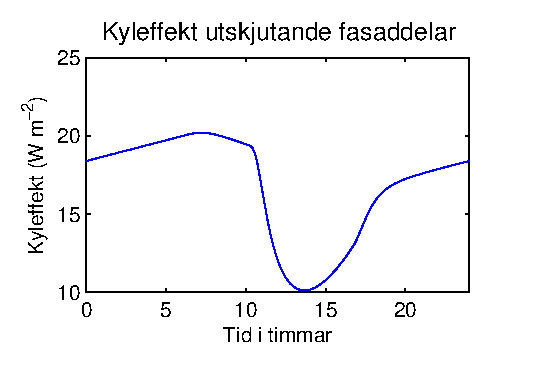
\includegraphics[width=6cm]{images/decsunbay.eps}
}
\subfloat[\label{fig:bursprak_dec} Energiflöde ut från insidan av burspråket en molnig dag i december.]{
	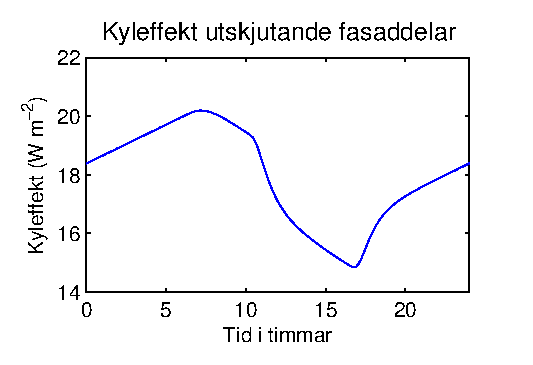
\includegraphics[width=6cm]{images/baynosundec.eps}
}
\caption{\label{fig:bursprak_energi} Energiflöden ut från insidan av en vägg. Utflöden ut genom burspråket betecknas positivt, och inflöden negativt. }
\end{figure}

Genom burspråket ser energiflödet lite annorlunda ut jämfört med det genom tegelväggarna,
se figur~\ref{fig:bursprak_energi}. En aprilmorgon innan solen har gått upp når energiflöde
sitt maximum med $\unit[10]{W~m^{-2}}$. När solen sedan värmer burspråket börjar energi
istället flöda in i byggnaden och en riktigt solig dag är det maximala inflödet över
$\unit[20]{W~m^{-2}}$, se figur~\ref{fig:bursprak_april1}. En molnig dag stannar det istället på ungefär $\unit[1]{W~m^{-2}}$ ut ur burspråket, se figur~\ref{fig:bursprak_april2}

En molnig dag i december är det betydligt kallare och energiutflödet varierar mellan 16 och
$\unit[21]{W~m^{-2}}$, se figur~\ref{fig:bursprak_dec}. En solig decemberdag är det tyvärr
inte mycket bättre och kyleffekten är alltid större än $\unit[10]{W~m^{-2}}$, se
figur~\ref{fig:bursprak_decsun}.
En intressant detalj är att kyleffekten på burspråket inte alls är sinusformad, på det vis som flödet genom väggarna i figur~\ref{fig:energyflow_stst} och \ref{fig:wall_dec} är. Det beror troligen på att burspråkets väggar är väldigt tunna och reagerar snabbt på förändringar.

%%%%%%%%TAKET%%%%%%%%%%%%%%%%%%%%%%%%%%%%%%%
\paragraph{Taket}


Energiflödet genom taket beräknas på samma sätt som energiflödet genom väggarna. Skillnaden, förutom materialet, är takets vinkel mot solen. I figur~\ref{fig:rooffiguressun} visas energiflödet för en solig april- respektive decemberdag. Eftersom taket lutar har nordsidan och sydsidan olika flöden ty solen skiner olika mycket på de olika lutade ytorna. Figur \ref{fig:rooffigurescloud} visar i sin tur situationen på molniga dagar, då ingen direkt solstrålning faller på taket.



\begin{figure}[hpbt]
\centering
\subfloat[\label{fig:roofaprilsunsouth} Energiflöde ut från insidan av sydsidan av taket en klar dag i april.]{
	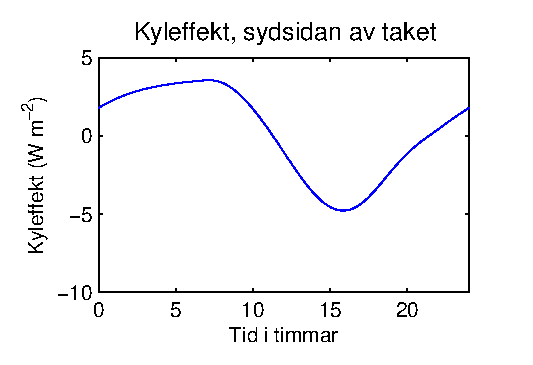
\includegraphics[width=6cm]{images/roofaprilsunsouth.eps}
}
\subfloat[\label{fig:roofaprilsunnorth}Energiflöde ut från insidan av norrsidan av taket en klar dag i april.]{
	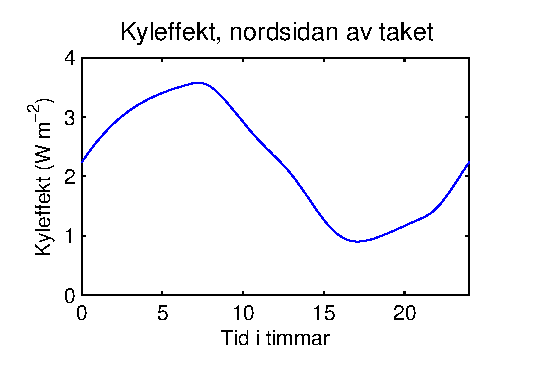
\includegraphics[width=6cm]{images/roofaprilsunnorth.eps}
}

\subfloat[\label{fig:roofdecsunsouth} Energiflöde ut från insidan av sydsidan av taket en klar dag i december.]{
	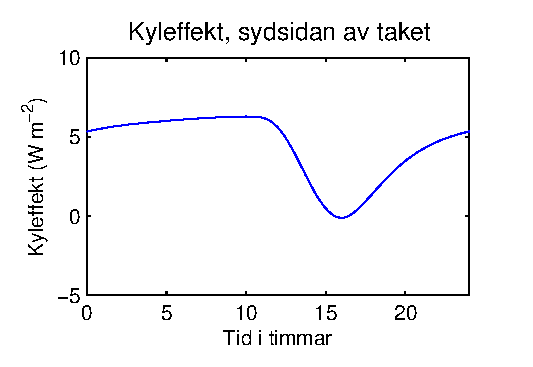
\includegraphics[width=6cm]{images/roofdecsunsouth.eps}
}
\subfloat[\label{fig:roofdecsunnorth} Energiflöde ut från insidan av nordsidan av taket en molnig dag i december.]{
	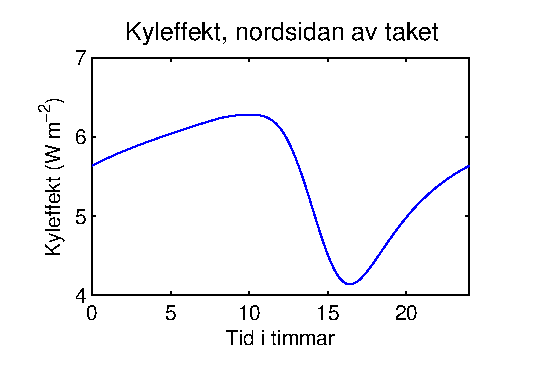
\includegraphics[width=6cm]{images/roofdecsunnorth.eps}
}

\caption{\label{fig:rooffiguressun}Energiflöden ut från insidan av en taket, klara dagar. Utflöden ut genom taket betecknas positivt, och inflöden negativt. }
\end{figure}

\begin{figure}[hpbt]
\centering
\subfloat[\label{fig:roofaprilnosun} Energiflödet från insidan av taket en molnig aprildag.]{
	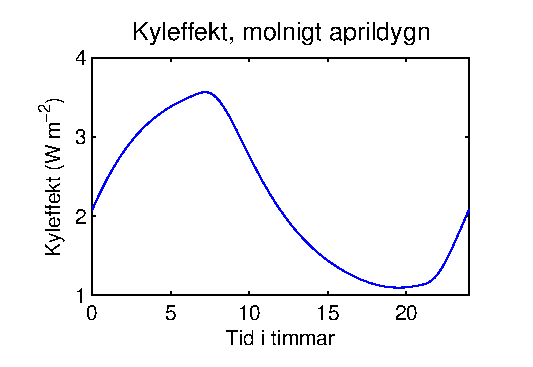
\includegraphics[width=6cm]{images/roofaprilnosun.eps}
}
\subfloat[\label{fig:roofdecnosun} Energiflödet från insidan av taket en molnig decemberdag.]{
	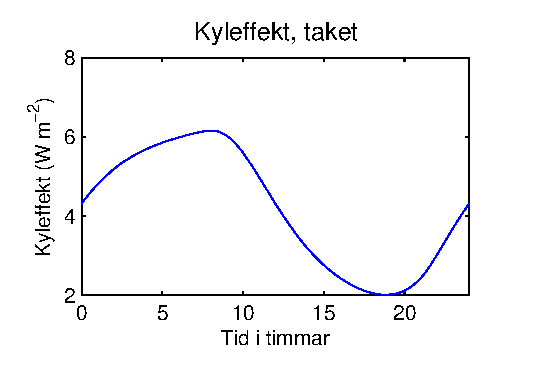
\includegraphics[width=6cm]{images/roofdecnosun.eps}
}

\caption{\label{fig:rooffigurescloud}Energiflöden ut från insidan av en taket, soliga dagar. Utflöden ut genom taket betecknas positivt, och inflöden negativt.}
\end{figure}

Energiflödet genom taket 
en klar dag i april varierar mellan $\unit[9]{W~m^{-2}}$ in och $\unit[3]{W~m^{-2}}$ ut på sydsidan, se figur~\ref{fig:roofaprilsunsouth}, 
och 
mellan $\unit[1]{W~m^{-2}}$ in och $\unit[3]{W~m^{-2}}$ ut på nordsidan, se figur~\ref{fig:roofaprilsunnorth}. 
Detta kan vidare jämföras med en molnig aprildag där utflödet varierar ännu mindre, bara mellan 0 och $\unit[3,5]{W~m^{-2}}$, se figur~\ref{fig:roofaprilnosun}. Solen har alltså stor en påverkan på energiflödets variationer.

En klar dag i december varierar energiflödet mellan 0 och drygt $\unit[5]{W~m^{-2}}$ ut ur taket på sydsidan och mellan drygt $\unit[4]{W~m^{-2}}$ och drygt $\unit[6]{W~m^{-2}}$ ut ur taket på nordsidan, se figur~\ref{roofdecsunsouth.eps} och \ref{roofdecsunnorth.eps}. En molnig dag i december varierar energiutflödet mellan 2 och $\unit[6]{W~m^{-2}}$, se figur~\ref{fig:roofdecnosun},


%%%%%%%%%%%%%%%%%%%%%%%%%%%%%%%%%%%%%%%%%%%%


\subsubsection{Flöde vid transient förlopp}

%To regerenate the figures use /code/pdesolver/calculateRisetime.m
%with the argument /code/pdesolver/wallstep.mat

\begin{figure}[hpbt]
\centering

\subfloat[Energiflöde ut från insidan av en vägg med $0,5\mbox{m}$ tegel.]{
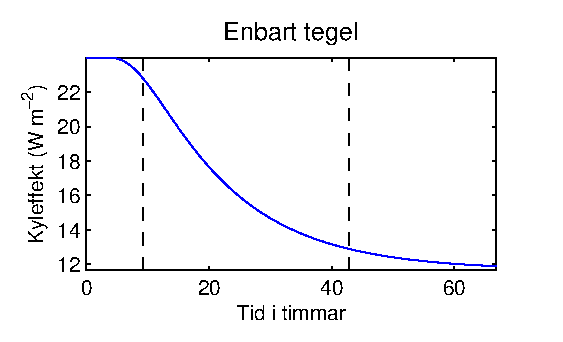
\includegraphics[width=6cm]{images/noinsulationstep.eps}
}\vspace{5mm}
\subfloat[Energiflöde ut från insidan av en vägg med $0,5\mbox{m}$ tegel och
$1\mbox{dm}$ tilläggsisolering bestående av mineralull.]{
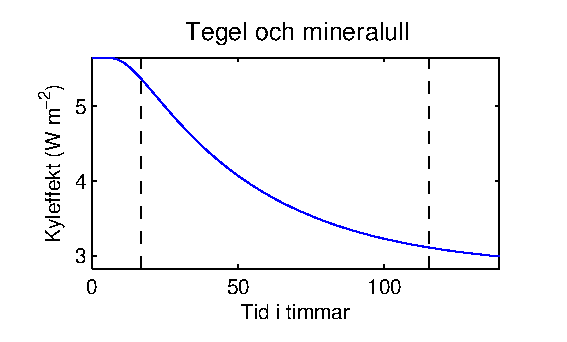
\includegraphics[width=6cm]{images/insulationstep.eps}
}
\caption{Energiflödet ut från insidan av en vägg där jämviktsläge med
$\unit[0]{^\circ C}$ på utsidan. Temperaturen förändras sedan
till $\unit[10]{^\circ C}$ vid tiden $t=0$. Insidan av väggen är satt till
konstanta $\unit[20]{^\circ C}$. De streckade linjerna markerar $\unit[10]{\%}$
fall samt $\unit[90]{\%}$ fall. Falltiden för dessa två väggar beräknades sedan
till $\unit[34,7704]{ timmar}$ för väggen utan isolering samt
$\unit[98,8372]{ timmar}$ för väggen med isolering. En annan intressant notering
är att det tog $\unit[9,5651]{ timmar}$ och $\unit[16,7533]{ timmar}$ för
energiflödet att falla $\unit[10]{\%}$. Beräkningarna är genomförda med finita
elementmetoden med $\unit[0,5]{m}$ tegel och $\unit[1]{dm}$ mineralull.}
\end{figure}


% \subsubsection{Luftfuktighetens inverkan på energiflöden}

\subsection{Luftflöde genom väggar – drag}

När det blåser på fastigheten får det luften kring fastigheten att cirkulera och även tränga in i 
byggnaden. När vinden ligger på med $\unit[3]{m/s}$, vinkelrätt mot nord- eller sydfasaden fås 
ett flöde som det i figur \ref{fig:windspeed} och trycket som då uppstår visas i figur 
\ref{fig:windpressure}. Tryckskillnaderna på de olika sidorna av husen kommer att driva 
ofrivillig ventilation vilket leder till energiförluster i form av infiltration.

\begin{figure}[hpbt]
\centering
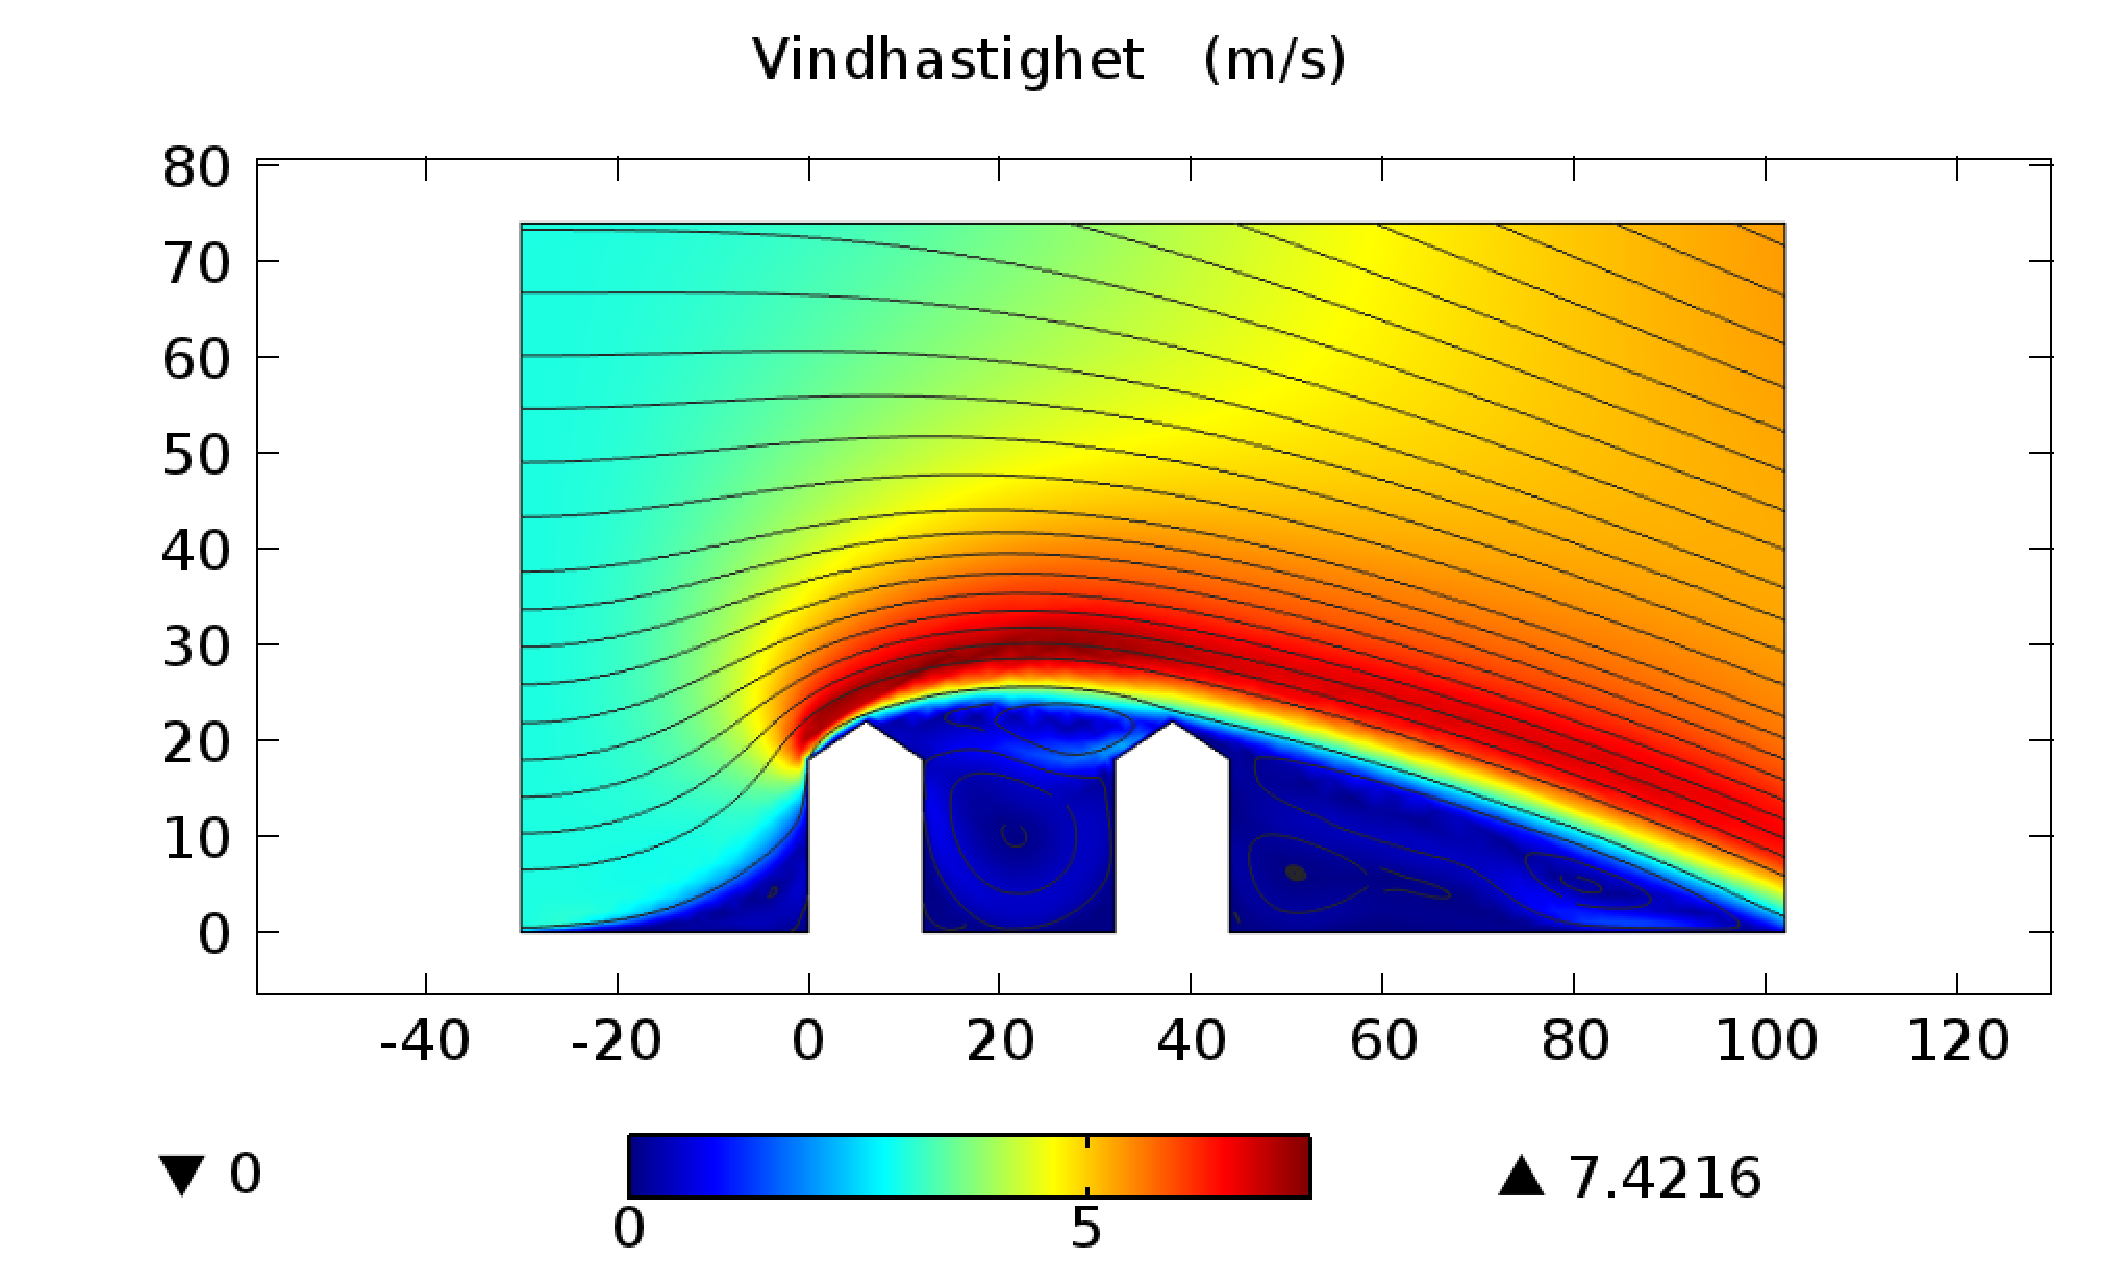
\includegraphics[width=127mm,height=76mm]{images/wind3mshdpi.eps}
\caption{\label{fig:windspeed}Vindhastiheten när vind i $\unit[3]{m/s}$ blåser mot fastigheten 
från vänster sida i figuren. Linjerna är strömlinjer och färgen indikerar farten. Värdena är 
framräknade med Comsol. Enhet m/s.}
\end{figure}


\begin{figure}[hpbt]
\centering
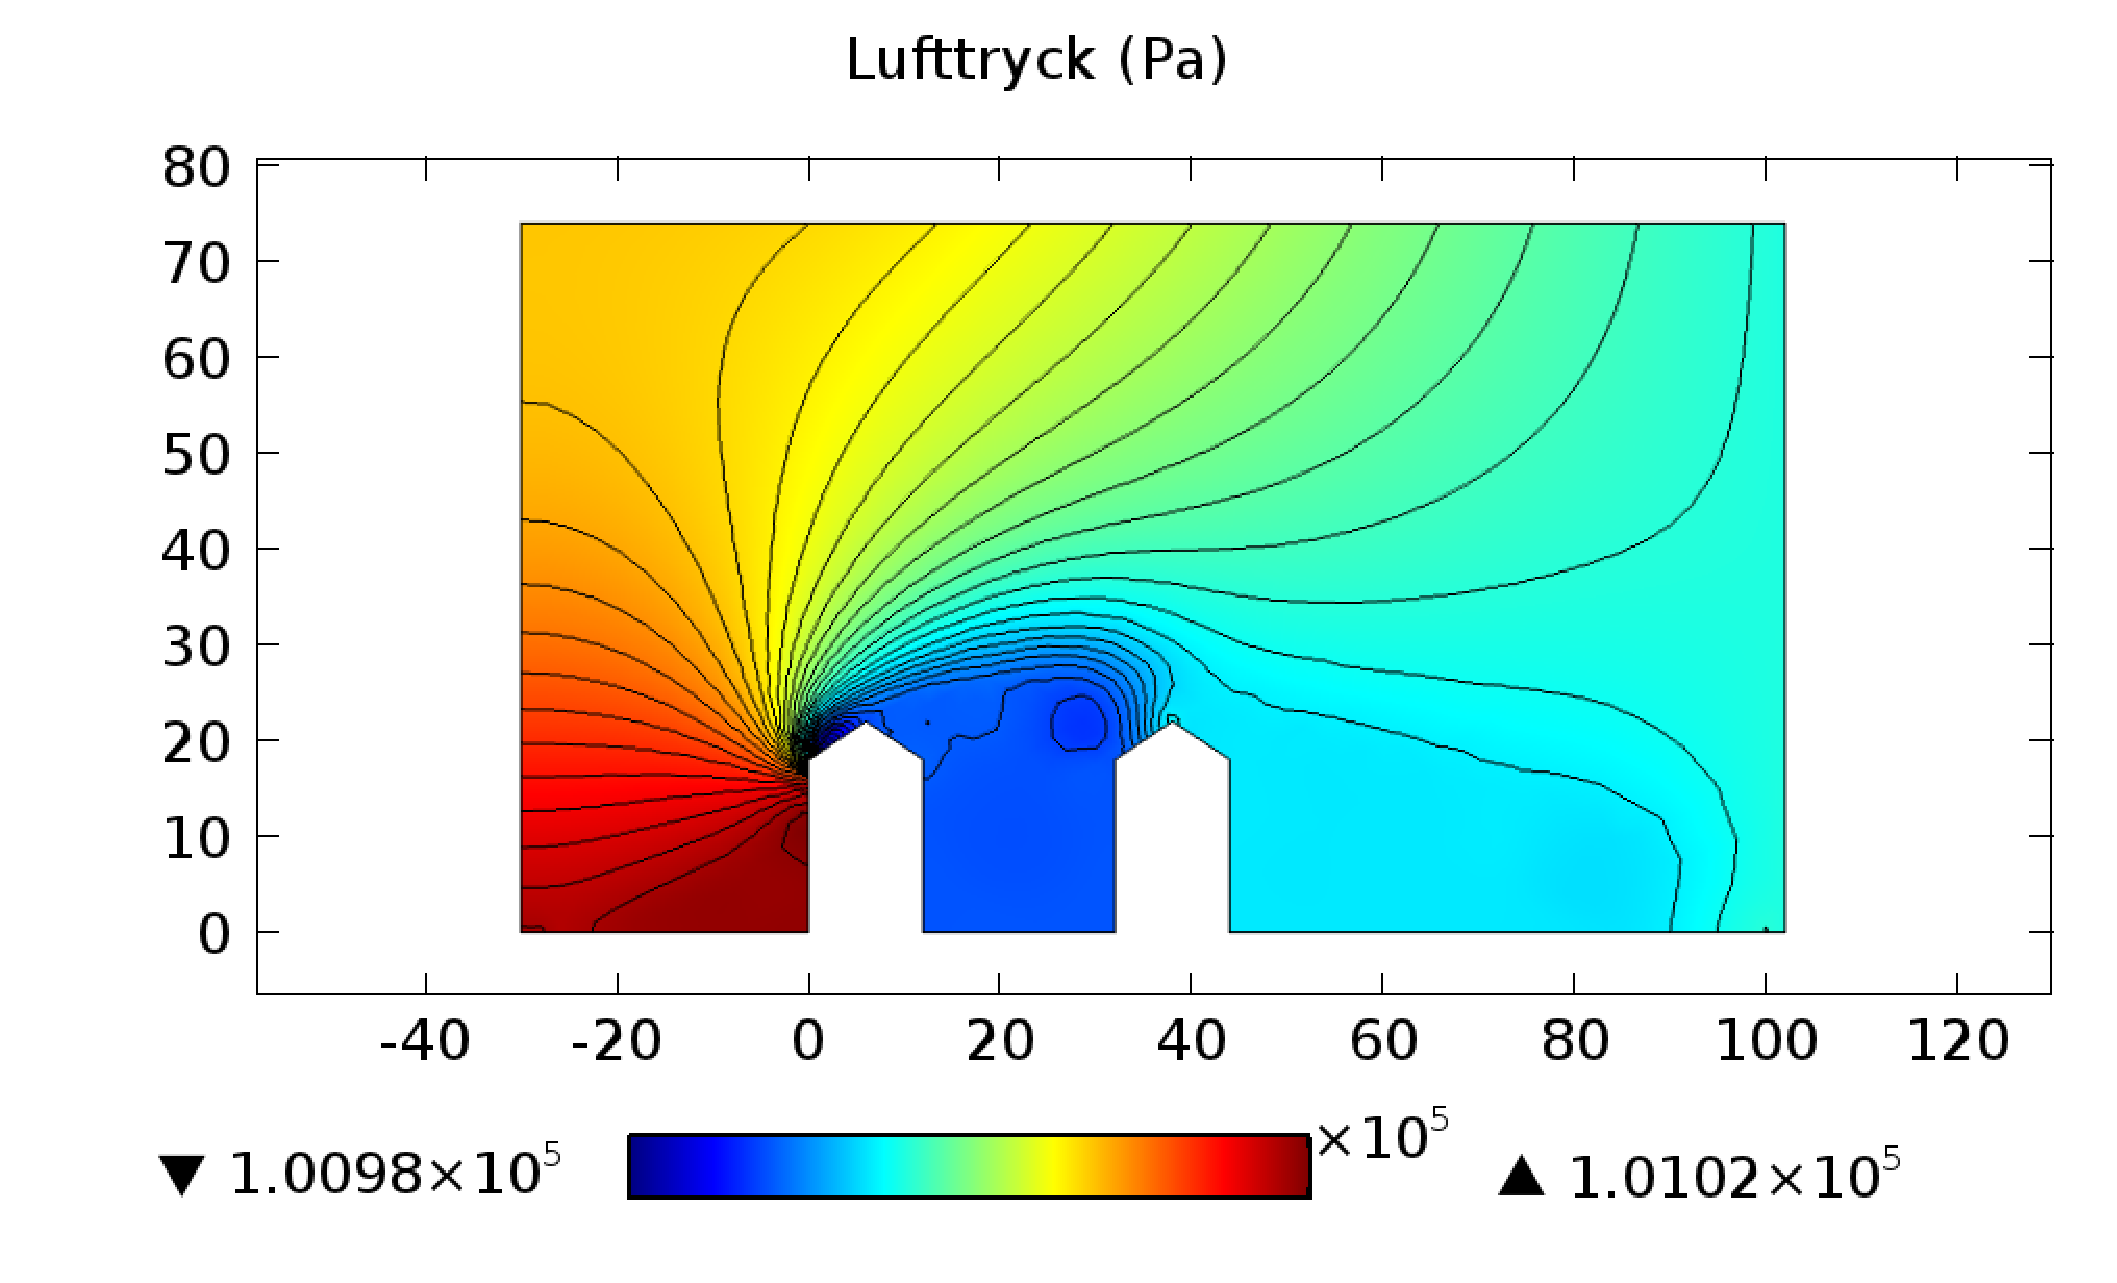
\includegraphics[width=127mm,height=76mm]{images/pressure3mshdpi.eps}

\caption{\label{fig:windpressure}Lufttrycket när vind i $\unit[3]{m/s}$ blåser mot fastigheten från vänster sida i figuren. Linjerna är isobarer, färgen indikerar lufttryck. Värdena är framräknade med Comsol. Enhet Pa.}
\end{figure}

% Resultat
Ur figur \ref{fig:windspeed} fås att det hus som ligger i lä utsätts inte för någon vind att tala om.
 Vidare fås ur figur \ref{fig:windpressure} att huset i lä utsätts för en betydligt mindre 
 tryckskillnad, än den byggnad som det blåser direkt på. I vårt exempel här, med en 
 vindhastighet runt $\unit[3]{m/s}$ fås en maximal tryckskillnad mellan norr- och sönderväggen 
 på 40 Pa, för fastigheten i lovart. Denna ökar när vindhastigheten ökar och vid 10 m/s fås en 
 tryckskillnad på 340 Pa för fastigheten i lovart. 

Applicerat på fastigheten på Walleriusgatan betyder detta att södervindar ger upphov till 
betydligt mer infiltrationsförluster än nordvindar. Till den aktuella byggnades fördel ska nämnas 
att södervindarna ofta är varmare än nordvindarna och de faktiska energiförlusterna blir 
troligen något mindre.

%%%%%%%%%%%%%%%%%%%%%%%%%%%%%%%%%%%%%%%%

Energiförlusterna på grund av drag har beräknats utifrån att en fix mängd energi per grad finns lagrad i en viss volym luft. Luftflödet genom väggen har beräknats på flera sätt. Både med Darcys lag och med byggfysikformeln, se avsnitt \ref{subsec:darcy}.

Energiförlusten har beräknats
  för en fastighet i lovart respektive en som ligger i lä av en annan byggnad, precis som 
  byggnaderna i figur \ref{fig:windspeed} och \ref{fig:windpressure}, vilket motsvarar att det 
  blåser på fastigheten på Walleriusgatan från söder respektive norr. Resultatet kan ses i figur 
  \ref{fig:windenergyloss} för en byggnad i lovart och en i lä samt för ett teoretiskt framtaget hus. Dessa två olika kurvor, framtagna med Darcys lag samt med en experimentell variant av densamma, får motsvara högsta respektive minsta gissningar för infiltrationsförluster i en byggnad.

Trycken är för figur \ref{fig:windenergylossa} och \ref{fig:windenergylossb} är framräknade för 
olika vindhastigheter med programmet Comsol medan det teoretiska modellen i figur 
\ref{fig:windenergylossc} är beräknat med med en approximation. 

Approximationen baserar sig
 på att tryckskillnaden mellan inne och ute är proportionerligt med vindhastigheten i kvadrat. Denna visar hur kyleffekten blir på en rätblocksformad byggnad som ligger helt ensam. Exakta kyleffekten beror väldigt mycket på vilken omgivning byggnaden står i.


\begin{figure}[hpbt]
\centering
\subfloat[\label{fig:windenergylossa}Byggnad som vinden blåser direkt på.]{
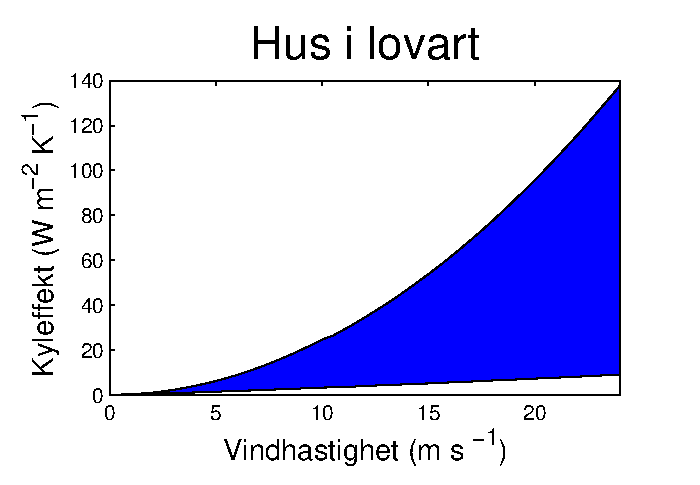
\includegraphics[width=60mm]{images/pressurewind.eps}}
\vspace{5mm}
\subfloat[\label{fig:windenergylossb}Byggnad som ligger i lä av en annan byggnad.]{
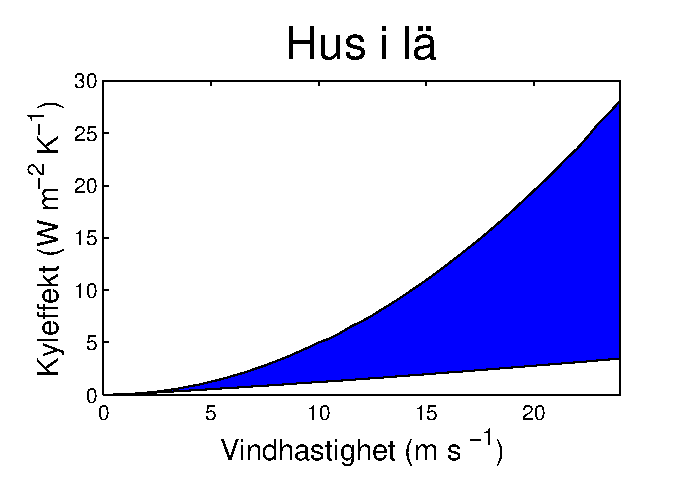
\includegraphics[width=60mm]{images/pressurenowind.eps}}

\subfloat[\label{fig:windenergylossc}Teoretisk approximation för lådformad byggnad.]{
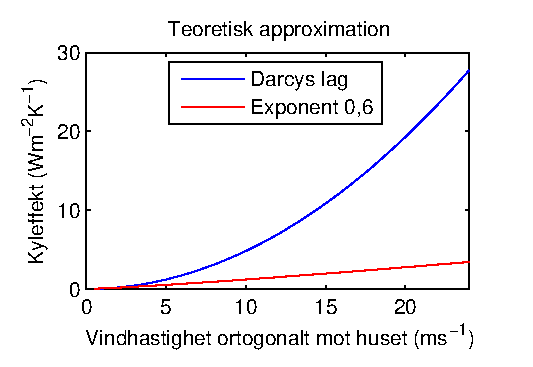
\includegraphics[width=60mm]{images/pressuretheory.eps}}

\caption{\label{fig:windenergyloss}Energiförlust per grad, max- respektive minvärde.
Framtaget med Comsol (a och b) och teoretiskt framräknade med en approximation (c).}
\end{figure}

% Resultat
Vilken kyleffekt vinden har på fastigheten är mer osäkert vid högre vindhastigheter. När vinden
 ligger på med upp emot 25 m/s kan kyleffekten variera från några tiotal watt per Kelvin upp 
 emot drygt hundra. Motsvarande kan kyleffekt för ett hus i lä vara mellan några watt per 
 Kelvin upp mot knappt trettio. För det teoretiskt beräknade huset fås även där att kyleffekten 
 kan vara mellan några watt per Kelvin upp mot knappt trettio dito. När vi har mer normala 10 
 m/s ser vi istället att kyleffekten kan vara från några få upp emot 20 W/K för en byggnad i 
 lovart, och ungefär en fjärdedel av det för en byggnad i lovart.



\subsection{Solstrålning genom fönster}

Exempel på resultat från beräkningar på solstrålning genom fönster. Beräknat via trial.m i code-mappen.

I figur \ref{fig:sun0101and0601} ses de relevanta vinklar som bildas av solens position den första april, 2012. Den blå linjen i figuren representerar solens vinkel relativt ett fönsters normal (då denna pekar i horisontell sydlig riktning) och kan användas för att uppskatta effekten som solinstrålning bidrar till. Om solens intensitet antas vara konstant $\unit{200}{W/m^2}$ beräknas denna effekt motsvara vad som visas i figur \ref{fig:effekt0101and0601}. Här antas fönstrets area uppgå till $\unit{1.5}{m^2}$, g-värdet för normal solstrålning är ? och värdet p i koden sätts till ?, ty fönstren i den avsedda byggnaden är av typ treglas utan ytbeläggningar.

\begin{figure}[hpbt]
\centering
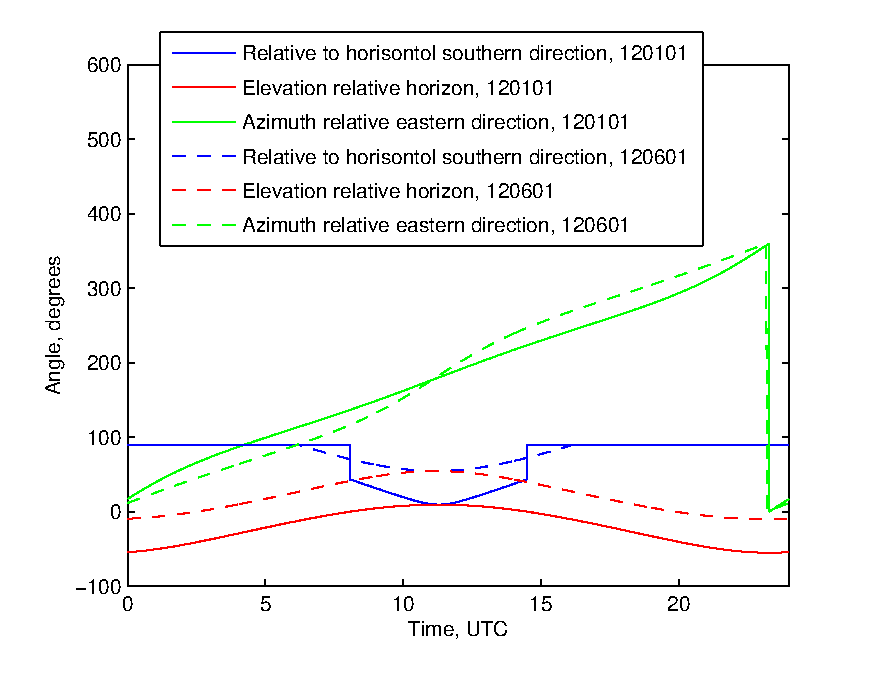
\includegraphics[scale=1]{images/sun0101and0601.eps}
\caption{\label{fig:sun0101and0601} Beräknade vinklar vid Walleriusgatan den första januari 2012 samt den första juni samma år, tid i UTC}
\end{figure}

\begin{figure}[hpbt]
\centering
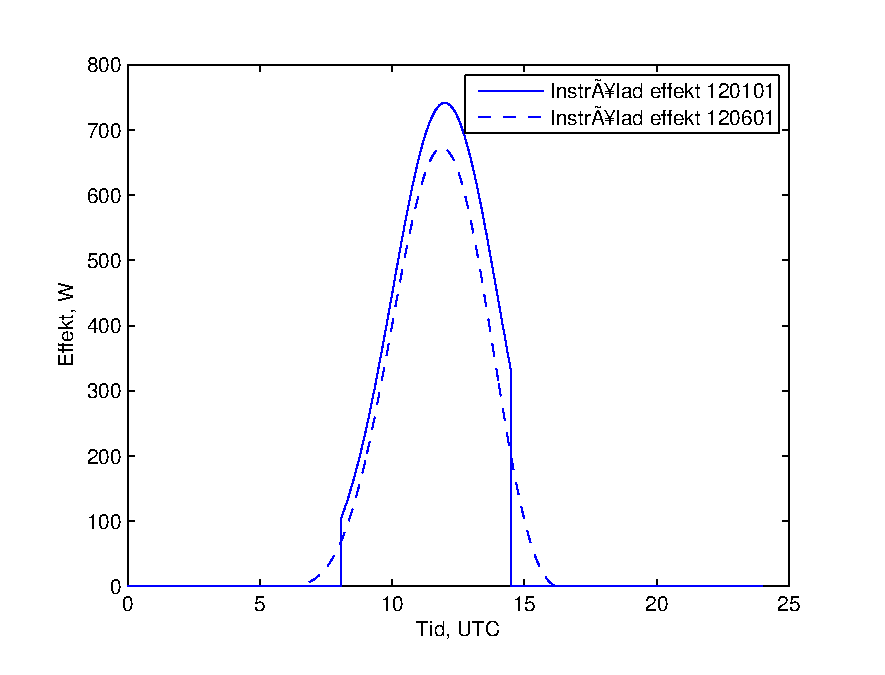
\includegraphics[scale=1]{images/effekt0101and0601.eps}
\caption{\label{fig:effekt0101and0601} Beräknad effekt genom ett fönster vars normal pekar i horisontella sydriktningen, den första januari 2012 samt den första juni samma år. Solens intensitet varierar under dagen enligt den blå kurvan.}
\end{figure}


\section{Energiflöde genom grunden}

% \subsubsection{Flöde vid termisk jämvikt}

Vid beräkningen av värmeflödet genom grunden användes geometrin som kan ses i figur \ref{fig:groundheat}.
Källaren antas vara belägen en halv meter under marknivån.

Som kan ses så varierar ej energiflödet så mycket mellan årstiderna och antags därför vara konstant i många applikationer.


\emph{\color{red} Nedanstående text måste göras om med de nya figurerna i åtanke,}
I samma figur ses även temperaturfördelningen vid termisk jämvikt då markens temperatur långt under huset sätts till konstanta $\unit[8]{^{circ}C}$. Vid markytan sattes konvektionskoefficienten till $h=\unit[15,5]{Wm^{-2}K^{-1}}$, motsvarande en ungefärlig vindhastighet (parallel med ytan) på $\unit[2]{ms^{-1}}$ vid utomhustemperaturen $\unit[0]{^{\circ}C}$. Källarens temperatur antas vara konstant $\unit[10]{^{\circ}C}$ och \textcolor{red}{grundens U-värde approximeras till $\unit[?]{Wm^{-2}K^{-1}}$}.


\begin{figure}
\centering
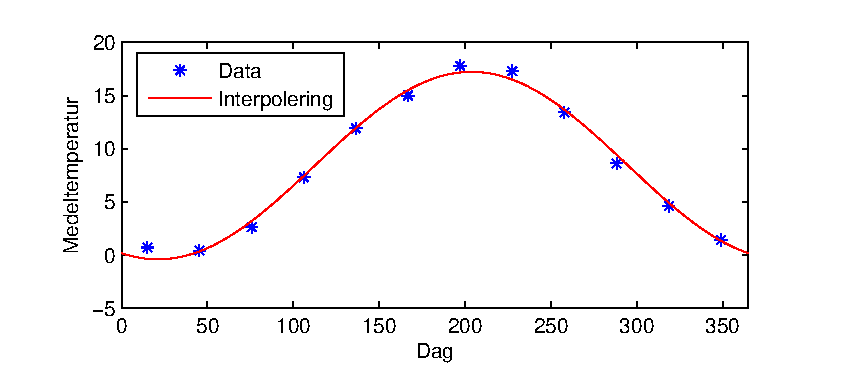
\includegraphics{images/meantemperature.eps}
\caption{Medeltemperaturen för göteborg de senaste 20 åren. Punkterna är data tagna från Miljöförvaltningen
och linjen är minstakvadratanpassningen som senare använts för att beräkna energiflöden.
\emph{\color{red} Denna graf kanske inte ska ligga här eller alls vara med. Metod möjligtvis? Vad tycker ni?}}
\end{figure}

\begin{figure}
\centering
\subfloat[Temperaturfördelningen i $^\circ\mbox{C}$ första januari.]{
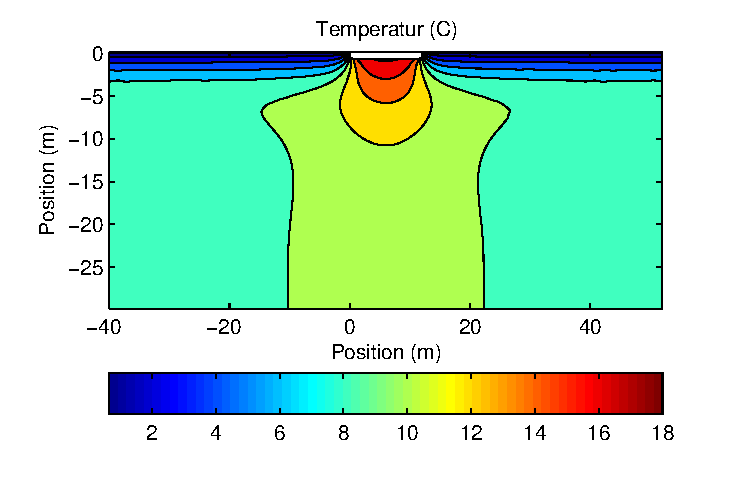
\includegraphics{images/groundheatdec.eps}
}

\subfloat[Temperaturfördelningen i $^\circ\mbox{C}$ första juli.]{
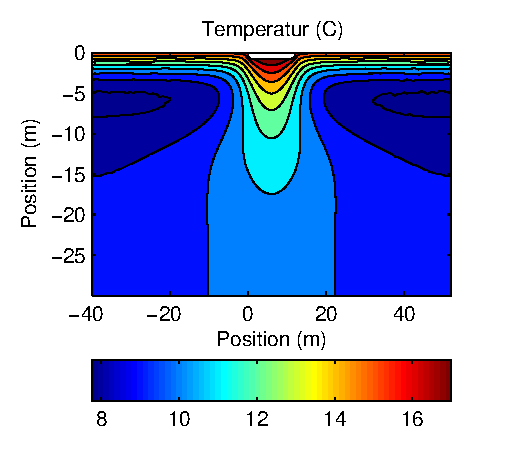
\includegraphics{images/groundheatjune.eps}
}
\caption{\label{fig:groundheat}Temperaturen i marken under en byggnad angivet i grader Celsius.
Temperaturfördelningarna skall motsvara två fiktiva dagar under ett år som är baserad på månadsmedeltemperaturen
de senaste 20 åren i Göteborg. Konvektionsparametern är satt till $h=15,5$. }
\end{figure}


\begin{figure}
\centering
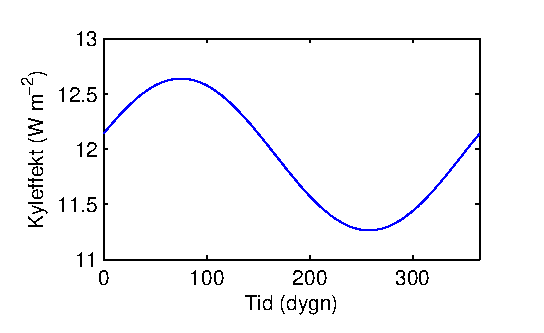
\includegraphics{images/groundcool.eps}
\caption{Kyleffekten per $m^2$ från grunden för medelåret de senaste tjugo åren. \emph{\color{red} Samma parametrar som figuren ovan.}\emph{\color{red}                                     
Detta är en viktig figur. Här kan ses att $\Delta Q = 1.5*22*13 = \unit[439]{W}$. Detta offsettas lätt genom att fler
människor befinner sig i fastigheten på vintern ty det är kallt ute eller fler kollar på tv istället för att sola.
Således finns det inget behov för att reglera framlednigstemperaturen för energiförluster från grunden. Kan antagas konstant
$\approx \unit[3,5]{kW}$. Låter denna siffra rimlig?}}

\end{figure}


% \subsubsection{Flöde vid transient förlopp}

Vid beräkningen av energiflödet genom grunden användes geometrin som kan ses i figur~\ref{fig:groundheat}. Källaren antas vara belägen en halv meter under marknivån. I resonomanget nedan kommer det att visa sig att marken reagerar så pass långsamt på temperaturförändringar att jämviktsläget är det enda relevanta. Ett transient förlopp är helt enkelt långt ifrån verkligheten.

Som kan ses i figur~\ref{fig:cooling_ground} så varierar inte energiflödet mer än en dryg watt per kvadratmeter mellan årstiderna och i många applikationer antas det därför vara konstant. Då vår grund är ungefär $\unit[22]{m}\cdot\unit[13]{m}=\unit[286]{m^2}$ ger detta ett energiutflöde mellan $\unit[3,6]{kW}$ på våren och $\unit[3,2]{kW}$ under tidig höst. 

\begin{figure}
\centering
\subfloat[Temperaturen i marken den första januari, $^\circ\mbox{C}$.]{
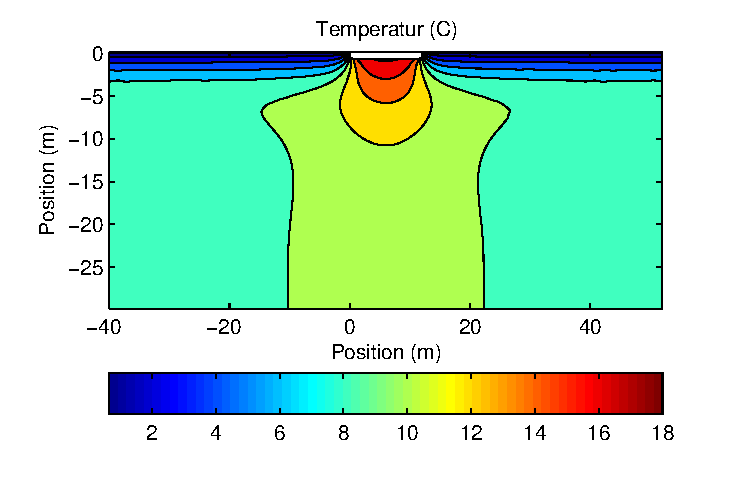
\includegraphics[width=7cm]{images/groundheatdec.eps}
}
\subfloat[Temperaturen i marken den första juli, $^\circ\mbox{C}$.]{
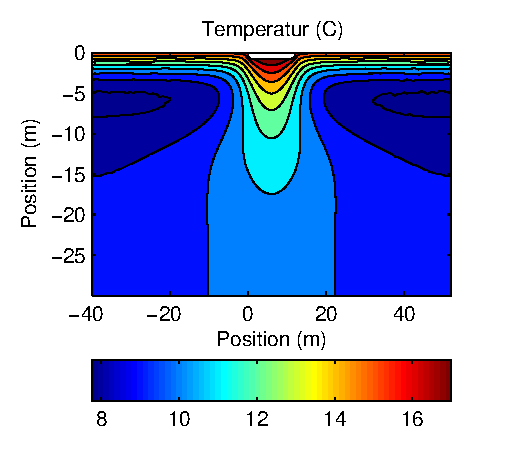
\includegraphics[width=7cm]{images/groundheatjune.eps}
}
\caption{\label{fig:groundheat}
Temperaturen i marken under byggnaden, $\unit{^\circ C}$, beräknat utifrån månadsmedeltemperaturen de senaste 20 åren i Göteborg för två fiktiva dagar i juni respektive januari. Konvektionsparametern är satt till $h=15,5$. }
\end{figure}


\begin{figure}
\centering
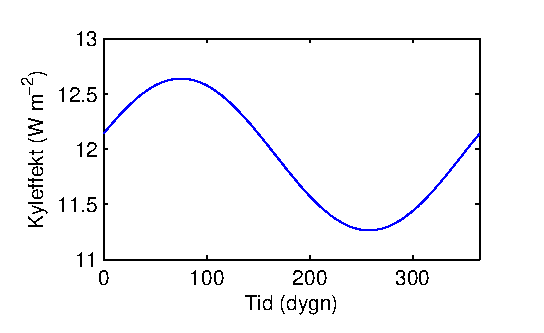
\includegraphics{images/groundcool.eps}
\caption{\label{fig:cooling_ground}
Kyleffekten per kvadratmeter från grunden för medelåret de senaste tjugo åren. Konvektionsparametern är satt till $h=15,5$. }

\end{figure}



% \section{Tidskonstanter}



\section{Sammanfattning av energiflöden: energibalanser}

\emph{\color{red} Jag är medveten om att mycket saknas och att det absolut inte är ett lämpligt sätt att sammanställa det på. Detta är ett försök till ett första utkast för att se vad det blir och vad som saknas. Eventuellt är det är helt fel tillvägagångssätt.}

De olika energiflödena är alltså från fasta energikällor, flöde genom väggarna, burspråk och tak, genom grunden, på grund av solinstrålning genom fönster samt på grund av ofrivillig ventilation.

Från fasta energikällor fås alltid ett bidrag på totalt $\unit[10,5]{kW}$, se avsnitt \ref{sec:constsources}.

Ur figurerna i avsnitt \ref{sec:steadystatewall} får vi energiflödena per kvadratmeter genom de olika avsnitten av klimatskalet och med hjälp av areorna i tabell \ref{tbl:uvalue} fås det totala energiutflödet genom husets hela klimatskal.

Flödet genom grunden fås ur figur \ref{fig:cooling_ground} och solinstrålningen genom fönster en solig dag fås ur figur \ref{fig:effekt0415and1231}.


\paragraph{I december:}
UTFLÖDET\\
Summa vägg, utan isolering –\\
\textbf{kl 5:} 6386+893+1994+6826=16099 W\\
\textbf{kl 15:} 5150+795+2001+7060=15006 W\\

Summa vägg, med isolering –\\
\textbf{kl 5:} 6386+893+1994+1671=10944 W\\
\textbf{kl 15:} 5150+795+2001+1680=9626 W\\

I december är energiutflödet genom grunden ungefär 12,1 W/m2. Grunden är 286 m2.\\
Energiutflödet genom grunden är 3461 W.

En molning dag i december sätts till 20\% av maximal instrålning, vilket ger $\unit[60]{Wm^{-2}}$. Utstrålning ur fönster?

Detta ger ett totalt energiflöde ut ur fastigheten en molnig, vindstilla, dag i december \textbf{kl 5:}\\
10500 - 16099 - 3461 = -9060 utan isolering.\\
10500 - 10944 - 3461 = -3905 med isolering.\\

Detta ger ett totalt energiflöde ut ur fastigheten en molnig, vindstilla, dag i december \textbf{kl 15:}\\
10500 -15006 - 3461 = -7967 utan isolering.\\
10500 - 9626 - 3461 = -2587 med isolering.\\

%%%%%%%%%%%%%%%%%%%%%%%%%%%%%%%%%%%%%%%

\paragraph{I april, soligt:}
UTFLÖDET\\
Summa vägg, utan isolering –\\
\textbf{kl 5:} 2884+470-228-1060=2066 W\\
\textbf{kl 15:} 2266-705-101+212=1672 W\\

Summa vägg, med isolering –\\
\textbf{kl 5:} 2884+470-228-191=2935 W\\
\textbf{kl 15:} 2266-705-101-85=1375 W\\

I april är energiutflödet genom grunden ungefär 12,5 W/m2. Grunden är 286 m2.\\
Energiutflödet genom grunden är 3575 W.

En solig dag i april sker ingen solinstrålning kl 5, men 540 W/m2 kl 15. Det motsvarar 0 W kl 5 respektive 81540 W in genom fönstren på södersidan.

Detta ger ett totalt energiflöde ut ur fastigheten en (solig) vindstilla, dag i april \textbf{kl 5:}\\
10500 - 2066 - 3575 =  4859 W, utan isolering.\\
10500 - 2935 - 3575 =  3990 W, med isolering.\\

Detta ger ett totalt energiflöde ut ur fastigheten en solig, dag i april \textbf{kl 15:}\\
10500 - 1672 - 3575 + 81540 = 86793 W utan isolering.\\
10500 - 1375 - 3575 + 81540  =  87090 W med isolering.\\


%%%%%%%%%%%%%%%%%%%%%%%%%%%%%%%%%%%%%%%

\paragraph{I april, molnigt:}
UTFLÖDET\\
Summa vägg, utan isolering –\\
\textbf{kl 5:} 2884+470-228-1060=2066 W\\
\textbf{kl 15:} 2266-705-101+212=1672 W\\

Summa vägg, med isolering –\\
\textbf{kl 5:} 2884+470-228-191=2935 W\\
\textbf{kl 15:} 2266-705-101-85=1375 W\\

I april är energiutflödet genom grunden ungefär 12,5 W/m2. Grunden är 286 m2.\\
Energiutflödet genom grunden är 3575 W.

En molning dag sker ingen solinstrålning genom rutan.

Detta ger ett totalt energiflöde ut ur fastigheten en solig, vindstilla, dag i april \textbf{kl 5:}\\
10500 - 2066 - 3575 =  4859 W, utan isolering.\\
10500 - 2935 - 3575 =  3990 W, med isolering.\\

Detta ger ett totalt energiflöde ut ur fastigheten en solig, dag i april \textbf{kl 15:}\\
10500 - 1672 - 3575 = 5253 W utan isolering.\\
10500 - 1375 - 3575  =  5550 W med isolering.\\

%%%%%%%%%%%%%%%%%%%%%%%%%%%%%%%%%%%%%%%%



%Diskussion
\section{Diskussion}

\section{Felkällor}\label{sec:errors}

% ELIMINERAT AVSNITT

Onoggrannheten i beräkningsmodellerna.

h-värdet är väldigt approximativt. Vind!

Alla approximationer – hur stora fel.



% Koppla mot avgränsningar.
% Vad har de här avgränsningarna lett till för fel.


\subsection{Problem som vi stött på}



\section{Jämförelse med andra energibesparande åtgärder}

En övergripande likhet mellan energibesparande åtgärder är att många av dem kostar pengar. Innan det går att överväga något av dessa alternativ måste det klargöras vilka mervärden eller biverkningar olika system ger samt hur de kan utnyttjas maximalt. De finns lösningar som lämpar sig bättre och sämre för specifika byggnader. I det här avsnittet kommer en diskussion föras angående fyra alternativ till det momentant väderbaserade system rapporten undersöker i övrigt.
Som vi kan se i resultatet påverkar vädret energiflödet ut genom byggnaden högst väsentligt. Enligt \ref{} beror det mest på vind och solinstrålning och dess effekter fördröjs inte av trögheten i väggarna, vilket var en av utgångspunkterna för vårt. Solinstrålningen går främst genom fönster, och vinden går in i otätheter och för på så sätt in kallare luft i byggnaden utan fördröjning.

\paragraph{Besparingar}
Under rubrikerna besparingar kommer det presenteras vilka olika former av besparingar, effekter eller andra fördelar man får av att investera i den presenterade energisparformen. All energi som används till bostadsuppvärmning enligt \cite{energideklaration} antas ligga under vinterhalvåret, då uppvärming förekommer. Det antas inte försvinna energi till kyla under sommarhalvåret.  [Resultat ylva].

\paragraph{Ekonomi}
Under rubriken kommer förutsättningar i ekonomin beskrivas. Den är väldigt approximativ då vi inte har haft befogenheter att begära in riktiga offerter från bygg samt installationsföretag, då detta kostar dem pengar, i form av tid, samt att vi inte ens haft för avsikt att använda offerten, vilket är allmänt ojuste.

Vi använder genomgående Payoff-metoden, väldigt förenklad, med vilken man visar hur myket en investering betalar sig. Metoden tar inte hänsyn till att det är olika stora investeringar, då det inte framgår vilken man kan spara mest pengar på, utan vilken som lönar sig snabbast. Det finns inget restvärde för någon av investeringarna. Beräkningarna har gjorts för mest positiva samt mest negativa möjliga utfall, vilket ger ett spann på ett antal år. Förenklingarna leder till att vi varken tittar på kalkylräntor eller en eventuell ränta i det fallet investeringen måste finansieras med ett banklån.

\begin{equation} \label{eq:payoff}
\text{Antalet år}=\frac{\text{Grundinvestering}}{\text{Sparat belopp per år}}
\end{equation}

\subsection{Tilläggsisolering}
Våra beräkningar visar att väggen inte absorberar tillräckligt mycket energi för att det ska vara värt att inte isolera den. Se figurer i avsnitt \ref{sec:steadystatewall}.
När man gjorde en omfattande renovering i slutet av 1980-talet byggde man en yttre tilläggsisolering, med tio centimeter mineralull på den norra sidan, \cite{arsredovisning} innebärande 26 \% av husets yta utåt, grunden borträknat. Isoleringen gav en ungefärlig faktor en fjärdedel på U-värdet.Vi ser här det låga u-värdet på norrväggen kontra det fortfarande höga på sydsidan. \ref{tbl:uvalue} Dessa differenser ger oss möjligheten att göra förbättringar där det inte är tillräckligt isolerat, det vill säga till exempel där U-värdet ligger över ett.

En isolering av både syd samt västväggen är en isolering av en yta om 212 $\unit{m^2}$, som rent teoretiskt skulle få ett bättre U-värde. Det innebär 21,8 \% av ytan på fastigheten där energi kan ledas ut. \ref{tbl:uvalue}.
En tilläggsisolering kan göras på två olika sätt, inifrån eller utifrån. Med båda metoderna finns för samt nackdelar. Båda metoderna innebär betydande insatser i fastigheten. Det finns dock mervärden att ta under beaktande. 

\paragraph{Besparingar}
Fasader behöver med jämna mellanrum renoveras, och i samband med ett projekt av de proportionerna får man en fasadrenovering. Svenskt tegel har en ungefärlig livslängd på 50 år\cite{magnus}, dock ska tegelfasaden ha renoverats med ny impregnering i samband med renoveringen 1988. Teglet i fastigheten har troligtvis även en bättre livslängd än 50 år, kvaliteten när huset byggdes motsvarar det danska teglet, och då handlar det om cirka 100 år. Det största mervärdet ur vår synvinkel, vilket också framgick vid beställning att temperaturerna i bostäderna blir mycket jämnare [Referens från resultat]. Det beror på, vilket nämns tidigare i kapitlet att fasaden inte fungerar som den buffert eller ”element” som man tror att den gör.

\paragraph{Tilläggsisolering utifrån}
En tilläggsisolering utifrån är ett ingrepp som medför en stor kostnad. Områdena som bedöms vara lämpliga att tilläggsisolera är alla väggar med tegelyta, då de inte har någon tilläggsisolering sedan tidigare och U-värdet skulle då kunna förändras på sammma sätt som norrsidan när den isolerades vid renoveringen. Då det är en betydande investering måste mervärden och andra kostnader som kan tänkas uppstå tas under beaktande. Fasader behöver med jämna mellanrum isoleras. beräknat det genomsnittliga U-värdet per kvadratmeter för både fallet utan ytterligare isolering samt ett fall med isolering av alla tegelytor. Det handlar om skillnader i det genomsnittliga U-värdet för hela huset på ZZ \%[Referens]

\paragraph{Tilläggsisolering inifrån}
En tilläggsisolering inifrån innebär ingrepp i lägenheterna, bland de boende. Det kan medföra komplikationer med personer som inte vill göra lägenheten mindre, vilket är en mindre bieffekt av projektet. Hurvida de boende behöver kompenseras för ingreppet genom dubbelt boende eller ekonomiskt är inte klarlagt, men det behövs ta ställning till. Ingreppet blir inte lika komplett som att isolera utifrån, man kan helt enkelt inte isolera lika stor yta då innerväggar samt golvplan ansluter mot ytterväggen och bildar köldbryggor utåt. Summering ger att den beräknade ytan att isolera blir mindre, nedåt endast hälften mot den tidigare angivna samt att en isolering inifrån troligtvis blir mindre kostsam, men undersökningar har inte gjorts.

\paragraph{Ekonomi}
Vi har inte räknat på en isolering inifrån då det inte har varit möjligt att få en offert eller prisförslag på ett sådant arbete. Det är inte heller möjligt att göra på grund av de boendes preferenser. Genom en tjänst på internet fick vi visserligen kontakt med ett byggföretag som hävdade att de skulle kunna göra arbetet för 200 000 kronor, vilket enligt lite uppskattningar över kostnader för material, arbetskraft byggställningar och så vidare framstår som väldigt billigt. Dock har vi en uppskattad besparingsmöjlighet på 25 \%, vilket ger pay-off tiden dryga 10 år, vilket för en sådan typ av investering får anses vara helt okej.

\subsection{Termostater på element}
Styrning av rumstemperatur via termostater på element, är den tredje åtgärden att diskutera. I dagsläget regleras flödet manuellt via vred under elementen. De ställs in av fastighetsskötaren och kan regleras upp eller ner om bostadsrättsinnehavaren är missnöjd med inomhusklimatet. Termostater finns både elektriska samt 
Elektriska termostater finns i olika varianter, men det är främst en ett koncept från Danfoss vi tittat på. Det finns i två varianter vilka ska gå att implementera på i princip alla befintliga uppvärmningssystem. Man ställer in temperaturen man vill ha i grader, antingen i det billigare systemet direkt på termostaterna via en lite lcd-display, eller i det dyrare systemet som fungerar trådlöst mot en huvudenhet med en större färgdisplay.
Båda systemen kan bryta tillförseln vid tillfälliga kyltoppar, till exempel vid vädring. Det går genom systemet att hålla lägre temperatur i vissa rum, till exempel sovrum. Systemen kan programmeras att ta hänsyn både till solinstrålning genom fönster samt sänka dag, natte eller semestertid, när ingen är hemma.

\paragraph{Sidoeffekt}
En bieffekt att energianvändningen kan öka om det finns tillräcklig med energi i systemet och de boende vill ha varmare än vad som i dagsläget erbjuds. Det är lätt att begränsa temperaturintervallet, men det kan skapa irritationer om de boende upplever fel temperatur och inte kan ändra den när de har fått ett fint system för det.

\paragraph{Ekonomi}
Det är tveksamt vilken längd man skulle kunna tänka sig på en avskrivning av det här slaget, men en  rimlig avskrivningstid är fem år då det innefattar ett datorbaserat system. I kostnaden har endast materialet tagits med, det vill säga termostater samt huvudenheter. Dessa komponenter skulle kosta föreningen knappa 100 000 kronor, och med en besparing på upp till 45 \% per år blir payoff-tiden endast 2,85 år. Det är ungefär motsvarande en halv rimlig avskrivningstid, vilket är en bra investering sett till de perspektiven.

\subsection{Miljöinformation}
I samband med ett system där de boende själva kan reglera temperaturen kan man behöva informera de boende på ett attraktivt sätt, meningen är ju att både kostnaden ska sjunka, samt att miljöpåverkan ska minskas. Börjar temperaturen då smyghöjas i lägenheterna blir så inte fallet, det börjar kosta mer i el, samt förslitning av pumpar m.m.  \cite{viivilla}


\subsection{Prognosstyrning}
Prognosstyrning är en möjligheten för att styra inomhustemperaturen efter vädret, vilket skulle kunna vara ett alternativ för byggnaden vi har studerat.
Fördelarna med prognosstyrning kontra att styra direkt mot väderstationen är att de flesta markanta väderpåverkningarna är momentana, det vill säga att det inte sker någon fördröjning innan de kommer in i byggnaden. Då krävs framförhållning för att kunna ta hänsyn till dessa, vilka är främst vind och solinstrålning, vilket kan ges av prognosstyrning. Sveriges meterologiska och hydrologiska institut, SMHI står för prognoserna som skickas till systemet, vilket i sin tur har installerats av deras samarbetspartner. En prognos skickas egentligen aldrig, utan det som skickas är en styrsignal som baseras på väderprognoser samt data om byggnadens energibalans som skickas till styrsystemet, som sedna försöker optimera energiåtgång och boendekomfort efter givna värden.

\paragraph{Besparingar}
SMHI påstår att det kan ge kostnadsbesparingar på 5-10 \% på uppvärmningen, och att förutsäga exakt hur mycket är väldigt svårt, då deras modell angående vilka parametrar styrningen beror på är kommersiell och således inte delges allmänheten. Antydningar från mötet med SMHI menade på att den här fastigheten inte låg i den övre delen av skalan, men det beror ju helt på hur olika parametrar viktas, och en korrektare bedömning kräver troligtvis att man har för avsikt att köpa det.

\subsection{Ekonomi}
Antalet år det tar innan en investering betalar sig enligt \ref{eq:payback} ges i tabell \ref{tbl:payback}

\begin{table}[hbtp]
\centering
\caption{Paybacktid för olika investeringar}
\label{tbl:payback}

\begin{tabular}
{|l|r|r|}
\hline
\textbf{Investering} & \textbf{Minimal paybacktid} &{\textbf{Maximal paybacktid} \\
\hline
Prognosstyrning &  1 & 2,9 \\ 
\hline
Väderstation & 1,7 & 5,2 \\
\hline
Termostater & 2,9 & 12,8 \\
\hline
Tilläggsisolering & 8,7 & 52,2 \\
\hline
\end{tabular}
\end{table}





\paragraph{Ekonomi}
Den stora fördelen med det här systemet är SMHIs prismodell. Den innebär att investeringskostnaden ska kunna betala sig inom två år, samt att abonnemangsavgiften inte är högre än maximalt hälften av vad man sparar varje år. Det är således väldigt intressant då man egentligen inte behöver några ekonomiska muskler för att börja använda produkten, även en förening som redan har mycket lån och nästan går med minus kan köpa systemet, för det blir billigare i vilket fall. Det bidrar till att samtidigt som SMHI kan ta betalt för sina prognoser, så sparar de boende pengar och mindre energi behöver produceras. SMHI lejer ut installationen till sina samarbetspartners. Systemet är enkelt och lätt att installera, vilket tillsammans med det låga priset bidrar till att göra det attraktivt.

Med sina två års payback-tid är prognosstyrning det alternativet som verkar bäst enligt payback-metoden. Här visar det sig att de största besparingarna dock inte alltid hittas med Paybackmetoden. Skulle föreningen investera i systemet, som man enligt SMHI ska kunna få installerat för cirka 10 000kronor, sparar man dock inte så mycket per år. Det är metoden med klart sämst förbättringspotential, samtidigt som SMHI kräver en abonnemangsavgift varje år, dock inte högre än runt 30 \% av vad man sparar


\section{Rekommendationer till fortsatt arbete}

Detta är det tredje arbetet som modellerat olika delar av fastigheten på Walleriusgatan för att
kvantifiera värderpåverkan. Detta har genomförts med olika metoder men slutsatserna från arbetena är ungefär desamma.
Därför känns det onödigt att genomföra ett fjärde arbete med samma infallsvinkel. Man kan bara komma så
långt med liknande metodik.

För fortsatt arbete rekommenderas att någon av två olika vägar väljs. De benämns
som produktspåret och grundforskningsspåret. Nedan följer en beskrivning av våra idéer kring dessa.

\paragraph{Produktspåret}
Uppdragsgivaren till detta projekt har som mål att helt automatisera värmeanläggningen i fastigheten och att stabilisera
temperaturen med avseende på väderpåverkan. För att genomföra detta behöver man implementera ett självförbättrande
reglertekniskt system, gärna i nära kontakt med industrin med sikte på att skapa en kommersiell produkt. 

Vid vårt möte med SMHI fick vi intrycket av att de skulle vara väldigt intresserade av att få data från fastigheten.
Detta inkluderar både data från värmeanläggningen och data från väderstationen. Därför kan det vara
en god idé att lägga fortsatta arbeten på is tills det finns några års data från fastigheten att tillgå.
Denna skulle då, tillsammans med erbjudande om ett kandidat- eller examensarbete, kunna bytas mot att få ett värmesystem implementerat till en låg kostnad. Datan skulle dessutom vara till stor nytta för att studera vad olika väder sk1apar för
krav på en värmeanläggning. 

Kompetensen som skulle krävas för ovanstående projekt ligger inom områdena reglerteknik, fysik, byggfysik samt vana med maskininlärning.
Dessutom skulle det vara en fördel om kompetens inom ekonomiska beräkningar finns inom projektgruppen för att
kunna tillgodose att produkten blir lönsam både för företaget och för kunden. Vi anser att detta skulle vara en god
idé till kandidat. eller examensarbete, dock med kravet att dessa kan samarbeta med
ett företag som håller på med denna typ av värmeanläggningar. Detta tror vi är nödvändigt för att projektet skall kunna mynna ut i en marknadsredo produkt.


\paragraph{Grundforskningsspåret}

De tidigare genomförda arbetena har enbart skummat lite på ytan angående vädrets påverkan på fastigheter och alla energiförluster
har kvantifierats väldigt approximativt. För att förbättra tidigare uppsattningar bör en djupare anayls av specifika energiförluster göras. Dessa skulle dock behöva vara kraftigt avgränsade. Några intressanta saker att studera
närmare är vädrets påverkan av konvektionsparametern. Detta skulle kunna genomföras med smarta experiment eller
med avancerade datormodeller. En annan idé är att närmare studera strålning som passerar genom byggnadens fönster. Till detta
skulle det krävas experiment eller data för fönstren för att få veta frekvensberoendet på absorbtions-, reflektions- samt
transmitanskoefficienterna. Med
denna data så skulle det sedan vara möjligt att räkna, alternativt modellera, strålningen genom fönstren. Detta skulle troligen
vara ett lämpligt projekt för några Fysik- och Kemiteknik-teknologer.

Om det skulle finnas några års data från fastighetens värmeanläggning samt väderstation så skulle det
även vara lämpligt att behandla denna med statistik. Genom att genomföra kan man förhoppningsvis
gå att få en ganska god bild över hur väder påverkar fastigheten i realiteten. Ett väl utfört arbete skulle
även kunna bidraga med ett recept för att göra liknande studier på andra fastigheter. Med lite tur skulle detta
kunna bidra med nya insikter i hur väder påverkar en fastighets uppvärmning och kunna leda till nya idéer angående
hur vädrets negativa inverkan kan minimeras och dess positiva inverkan utnyttjas maximalt.


\section{Tillämpningar}

De två primära tillämpningarna av det här arbetet är att identifiera energiläckor för att kunna göra sitt hus mer energieffektivt och att låta sitt energiförsörjningssystem vara väderberoende.

Att energieffektivisera sitt hus kan, om man väljer rätt metod, löna sig både ekonomiskt och miljömässigt. Det leder dessutom till mindre fluktuationer i inomhustemperaturen, speciellt om man har stor tröghet i sitt uppvärmningssystem.

Att låta energiförsörjningssystemet bero av väderdata från en vid fastigheten monterad väderstation kräver experimentella mätning på den aktuella fastigheten för att bli implementerbart.
Dessutom kommer direkta eneriflöden, så som solinstrålning och vind, att kompenseras för fördröjt, vilket kan bli ett problem om man har ett långsamt system för uppvärmning. Ett alternativ då är prognosstyrning men de färdiga system som finns på marknaden idag är så pass bra att det inte är av intresse att försöka bygga ett eget, inte ur ekonomisk synvinkel i alla fall.



%Slutsats
\subsection{Slutsats och diskussion}

\begin{frame}{Sammanfattning av energiflöden\\En klar decemberdag}


\begin{figure}
        \begin{subfigure}[b]{0.55\textwidth}
                \centering
                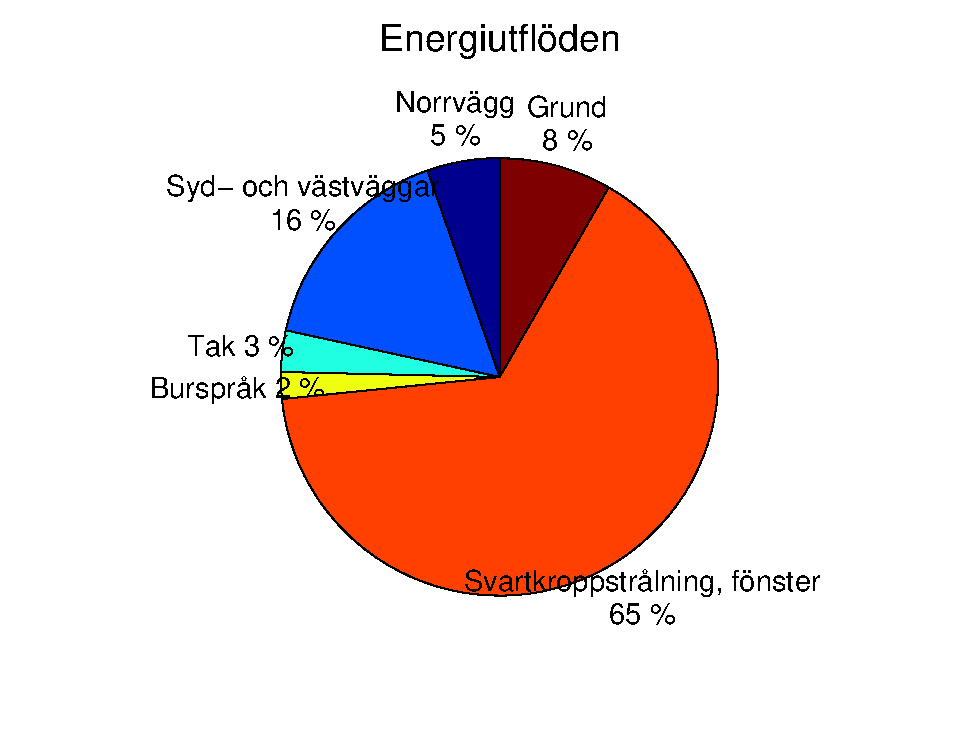
\includegraphics[width=\textwidth]{images/totalflow_out.eps}
                \caption*{Totalt 42 kWh/dygn \\ ~}
        \end{subfigure}
        \hskip-1.5cm
        	\uncover<2>{
        \begin{subfigure}[b]{0.55\textwidth}
                \centering
                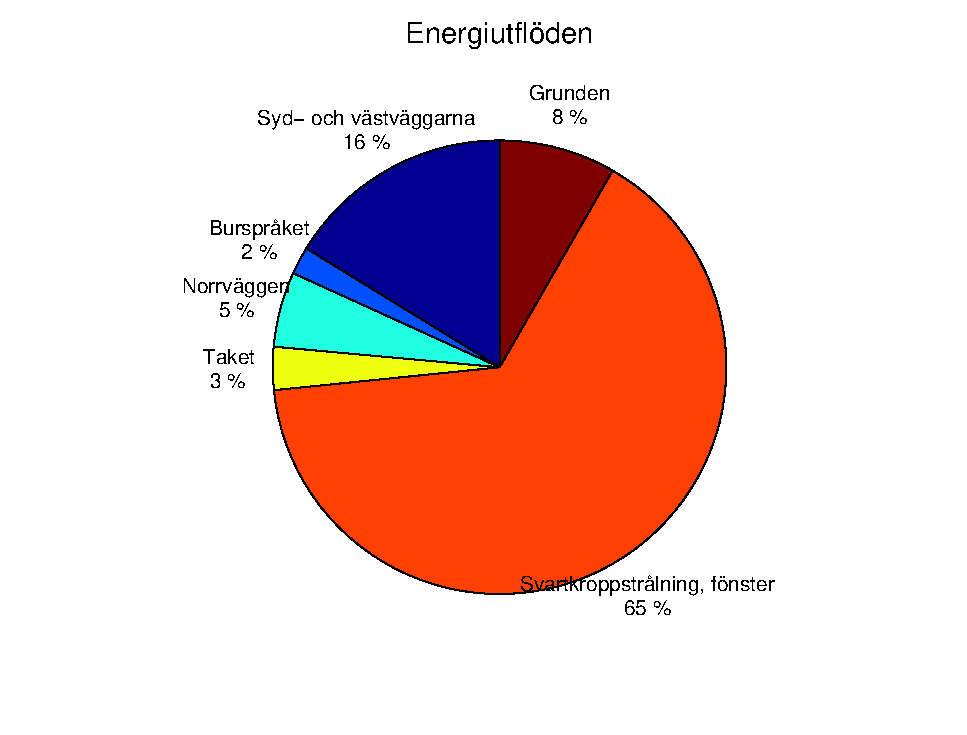
\includegraphics[width=\textwidth]{images/totalflow_in.eps}
                \caption*{Totalt 16 kWh/dygn \\+ tillförd energi}
        \end{subfigure}
        }
\end{figure}

\end{frame}


%\input{}


%---
\newpage
\clearpage
\addcontentsline{toc}{chapter}{Referenser}
\bibliography{ref}{}
\bibliographystyle{plain}
\newpage
\appendix

\chapter{Formler för linjära triangulära element}
\label{sec:integrationformulae}
\rhead{Appendix \ref{sec:integrationformulae}}

Vid skapande av stelhetsmatriser och lastvektorer behövs ett antal integraler
evaluras. Detta appendix syftar till att vara en formelsamling för några
nödvändiga beräkningar för linjära triangulära element. I ekvation
\eqref{eq:formula:area} beskrivs arean av en triangel. $(x,y)$ betecknar koordinaterna
av hörnen $(i,j,k)$. Ekvation \eqref{eq:formula:volume} beskriver integralen för ett
antal basfunktioner $\phi$ över en triangel $\Omega$. Liknande formulering för två dimensioner
återfinns i ekvation \eqref{eq:formula:rand}. I denna betecknas linjen mellan kanterna
$i$ och $j$ som $\Gamma$. \cite{lewis04}

Slutligen förekommer det även derivator av basfunktionerna. Alla derivator i en triangel
kan med lätthet beräknas genom att använda en determinant enligt ekvation
\eqref{eq:formula:derivative}. Här löper $l$ över $l=i,j,k$ och $\mathbf{r} = (x,y)$ som är
de rumsliga koordinaterna. \cite{fem50}

\begin{align}
\label{eq:formula:area}
A &=
\frac{1}{2}
\begin{vmatrix}
1 & 1 & 1 \\
x_i & x_j & x_k \\
y_i & y_j & y_K
\end{vmatrix} \\
\label{eq:formula:volume}
\int_\Omega \phi^a_i\phi^b_j\phi^c_j d\Omega &=
\frac{a!b!c!2A}{(a+b+c+2)!} \\
\label{eq:formula:rand}
\int_\Gamma \phi^a_i \phi^b_j d\Gamma &=
\frac{a!b!l}{(a+b+1)!} \\
\label{eq:formula:derivative}
\frac{\partial \phi_l}{\partial \mathbf{r} } &=
\begin{pmatrix}
1 & 1 & 1 \\
x_i & x_j & x_k \\
y_i & y_j & y_k  
\end{pmatrix}^{-1}
\begin{pmatrix}
0 & 0 \\
1 & 0 \\
0 & 1
\end{pmatrix}
\end{align}


\newpage
\chapter{Matlab-kod}
\label{sec:mcode}

%\rhead{Appendix \ref{sec:mcode}}

\section{Beräkning av solens position}\label{app:sunposition}

\lstinputlisting{../code/sun/sunposition.m}

\section{Beräkning av effekt genom fönster}\label{app:sunwindows}
\lstinputlisting{../code/sun/angletheta.m}

\lstinputlisting{../code/sun/gvalue.m}

\lstinputlisting{../code/sun/effekt.m}

\section{Finita element av energiflöde genom grund}\label{app:femfoundation}

\lstinputlisting{../code/pdesolver/groundheatfemtransientanalys.m}

\lstinputlisting{../code/pdesolver/triarea.m}

\lstinputlisting{../code/getMeanTemp.m}

\lstinputlisting{../code/pdesolver/laplacestiff.m}

%\documentclass[12pt,a4paper]{article}
\usepackage[utf8]{inputenc}
\usepackage[T1]{fontenc}
\usepackage[swedish, english]{babel}
\usepackage{amsmath}
\usepackage{ae}
\usepackage{subfig}
\usepackage{units}
\usepackage{icomma}
\usepackage{color}
\usepackage{graphicx}
\usepackage{bbm}
\usepackage{textcomp}
\usepackage{float}
\usepackage{units}
\usepackage{amssymb}
\newcommand{\rd}{\ensuremath{\mathrm{d}}}
\usepackage{fullpage}

\newcommand{\id}{\ensuremath{\,\rd}}
\usepackage{hyperref}

% Ökar styckeavstånd
\setlength{\parskip}{2ex plus0.5ex minus0.2ex}
% Tar bort indrag i början av stycke
\addtolength{\parindent}{-0.6 cm}

\begin{document}
\selectlanguage{swedish}

\section*{Arbetsfördelning under projektet}

\emph{\color{red}Här kan ni fylla i vem som gjort vad.}
\emph{\color{red}Ny mall, nya grejer. Jag tycker/jag skulle vilja skriva ett löpande stycke under varje av de tre paragrapherna. När ni har gjort det, om ni tycker det är en bra idee, ta bort punktlistorna. Man kan själklart även skriva i punktlisteform, vad är bäst ?}

\paragraph{Ansvarsområden}

       Planering

       Informationsinhämtning/inläsningsdel

       Metoder -- val/utveckling 

       Genomförande 

\paragraph{Bidrag till problemlösning, syntes och analys}

       Problemlösning 

       Kreativitet, idérikedom

       Skapande av modell

       Analys av projektrelaterat material 

       Diskussionsbidrag

       Slutsatser 

\paragraph{Huvudansvarig författare av avsnitt}

       Avsnitten anges

       Eventuell redaktionell ansvarsfördelning bör anges"

\subsection*{Erik Ahlqvist}

\paragraph{Ansvarsområden}

\begin{itemize}
\item[-] Lagt mycket tid på inläsning av tidigare kandidatarbeten samt patent. Även en del artiklar, avhandlingar samt viss kurslitteratur. 
\item[-] Deltagit i planeringen, samt stor del skrivande i planeringsrapporten.
\item[-] Metoden för att göra ekonomiska uppskattningar.
\item[-] Hämtat all information kring andra energibesparande åtgärder. 
\end{itemize}


\paragraph{Bidrag till problemlösning, syntes och analys}

\begin{itemize}
\item[-] Deltagit i arbetet med att skriva om konduktion.
\item[-] Aktivt bidragit till att bygga upp en vettig diskussion, påverka innehållet och summera ihop det.
\item[-] Genom arbetet med diskussionen tagit en naturligt stor del även vid summeringen i slutsatserna.
\end{itemize}


\paragraph{Huvudansvarig författare av avsnitt}

\begin{itemize}
\item[-] 
\item[-] Huvudansvarig för hela jämförelsen med andra energibesparande åtgärder.
\item[-] Skrivit många utkast till resten av diskussion samt slutsats.
\end{itemize}




\subsection*{Ylva Dahl}

\paragraph{Ansvarsområden}

\item[-] Läst på om fastigheten och dess väderstation.
\item[-] Studerat in begreppen svartkroppsstrålning, free-running temperature, ekvivalent temperatur samt sökt information kring naturkonstanter för luft.
\item[-] Samlat in och sammanställt väderdata främst från SMHI:s databas för våra exempel.

\paragraph{Bidrag till problemlösning, syntes och analys}
\item[-] Summerat energiflöden.

\paragraph{Huvudansvarig författare av avsnitt}

\begin{itemize}
\item[-] Skrivit om fastigheten och dess väderstation.
\item[-] Presenterat naturkonstanter för luft och begreppen svartkroppsstrålning, free-running temperature och ekvivalent temperatur.
\item[-] Skrivit text till bilderna i resultatet – väggar, burspråk, tak och grund – och sammanfattat i bild och text.
\item[-] Skrivit dispositionen och introduktioner till avsnitten teori och resultat.
\end{itemize}


\subsection*{Mats Lindström}

\paragraph{Ansvarsområden}

\paragraph{Bidrag till problemlösning, syntes och analys}

\paragraph{Huvudansvarig författare av avsnitt}


\paragraph{Mats Lindström}
\begin{itemize}
\item A
\item B
\item ...
\end{itemize}



\subsection*{Dan Ståby}

\paragraph{Ansvarsområden}

\paragraph{Bidrag till problemlösning, syntes och analys}

\paragraph{Huvudansvarig författare av avsnitt}

\paragraph{Dan Ståby}
\begin{itemize}
\item Förstuderat samt implementerat finita-elementlösningarna av de studerade situationerna.
\item Skrivit textern om finita-elementmetoden i rapporten samt skrivit om närliggande ämnen som problemuppställning och dylikt. 
\item Implementerat Matlab-kod för att snyggt presentera data från datormodellerna samt producerat alla grafer från
nyss nämnda modeller.
\end{itemize}

\end{document}

%Add a new page between each appendix

\end{document}
